\documentclass[a4paper, 12pt, ngerman, twoside, openright]{scrreprt}

% Rendering packages
\usepackage{amsmath}
\usepackage{amssymb}
\usepackage{graphicx}
\usepackage{color}
\usepackage{fancyvrb}

% Page dimensions
\usepackage[inner=3.5cm,outer=2.5cm,top=3.7cm,bottom=3.5cm]{geometry} % Settings for twoside documents.
\usepackage{parskip}

% Font styling
\usepackage[ngerman]{babel}
\usepackage[utf8]{inputenc}
\usepackage[T1]{fontenc}
\usepackage{lmodern}
\renewcommand\familydefault{\sfdefault}

% Tables
\usepackage{tabularx}
\usepackage{tabulary}
\usepackage{longtable, lscape}

% Headers
\usepackage{scrpage2}  % header and footer for KOMA-Script
\pagestyle{scrheadings}
\automark[section]{chapter}
\usepackage{marvosym} % für Euro-Zeichen

% Zitate
\usepackage[backend=bibtex, style=numeric, sorting=none]{biblatex}
\usepackage[babel,german=guillemets]{csquotes}
\bibliography{Bibliothek/Bibliothek}

\usepackage[hyperindex,breaklinks,colorlinks=true,linkcolor=black,urlcolor=blue,citecolor=black]{hyperref}

% Code Blöcke
\usepackage{listings}

% Listings konfigurieren.
\lstset{language=[Objective]C, 
        breakindent=40pt, 
        breaklines, 
        frame=lines,
        morekeywords={id, Class, SEL, IMP, BOOL, nil, Nil, NO, YES,
                  oneway, in, out, inout, bycopy, byref,
                  self, super, _cmd,
                  @required, @optional,
                  @try, @throw, @catch, @finally,
                  @synchronized, @property, @synthesize, @dynamic},
        basicstyle=\ttfamily\scriptsize,
        literate=
            {Ö}{{\"O}}1
            {Ä}{{\"A}}1
            {Ü}{{\"U}}1
            {ß}{{\ss}}2
            {ü}{{\"u}}1
            {ä}{{\"a}}1
            {ö}{{\"o}}1}
        
\definecolor{dkgreen}{rgb}{0,0.6,0}
\definecolor{gray}{rgb}{0.5,0.5,0.5}
\definecolor{mauve}{rgb}{0.58,0,0.82}
\definecolor{orange}{rgb}{1,0.35,0.2}
\definecolor{lightblue}{rgb}{0.53,0.81,0.98}        

\lstset{frame=tb,
	language=Java,
	aboveskip=3mm,
	belowskip=3mm,
	showstringspaces=false,
	columns=flexible,
	basicstyle={\small\ttfamily},
	numbers=none,
	numberstyle=\tiny\color{gray},
	keywordstyle=\color{blue},
	commentstyle=\color{dkgreen},
	stringstyle=\color{mauve},
	breaklines=true,
	breakatwhitespace=true,
	tabsize=3
}

\lstdefinelanguage{drools}{frame=tb,
	morekeywords={rule, rule, when,then, end, end}
	aboveskip=3mm,
	belowskip=3mm,
	showstringspaces=false,
	columns=flexible,
	basicstyle={\small\ttfamily},
	numbers=none,
	numberstyle=\tiny\color{lightblue},
	keywordstyle=\color{orange},
	breaklines=true,
	breakatwhitespace=true,
	tabsize=4}

%NEW COMMANDS
\newcommand\tab[1][1cm]{\hspace*{#1}}

%Verfickte Glossare
\usepackage[nonumberlist,acronym,toc]{glossaries}
\makeglossaries
\newacronym[]{BSP}{BSP}{Beispiel Abkürzung}

\newglossaryentry{Beispiel Glossary Entry}
{
  name=Constrain-Satisfaction-Problem,
  description={Ein Constraint-Satisfaction-Problem besteht aus einer Menge von Variablen, ihren Wertebereichen und den Bedingungen, die Verknüpfungen zwischen den Variablen herstellen und dadurch festlegen, welche Kombinationen von Werten der Variablen zulässig sind}
}



\begin{document}



% Titelseite einfügen.
%Titelseite
% Seitennummer aus
\thispagestyle{empty}

\begin{titlepage}

\vspace{3cm}

\begin{center}
	%\includegraphics[scale=0.8]{Titelseite/Logo.pdf}  
\end{center}

\vspace{2.5cm}

\begin{center}
  \Large FAKULTÄT FÜR INFORMATIK
\end{center}

\vspace{1cm}
\begin{center}
	\Huge
	\textbf{Master Arbeit}\\
\end{center}

\vspace{1cm}

\begin{center}
	\Large
	\textbf{Digitalisierung im Handwerk}
\end{center}

\vspace{1.5cm}

\begin{center}
	\Large
	Fabian Kloos
\end{center}

\vspace{3.5cm}

\begin{center}
    \large
	\textbf{Betreuer}
\end{center}

\vspace{0.3cm}

\begin{center}
    \large
    bla bla bla Betreuer
\end{center}

\newpage
\thispagestyle{empty}
\mbox{}
\end{titlepage}


% Counter zurücksetzen. Römische Ziffern einstellen.
\pagenumbering{Roman}
\setcounter{page}{1}

% Selbständigkeitserklärung einfügen.
\chapter*{Selbstständigkeitserklärung}
Hiermit erkläre ich, dass ich die Arbeit selbständig verfasst, noch nicht anderweitig für Prüfungszwecke vorgelegt, keine anderen als die angegebenen Quellen oder Hilfsmittel benützt, sowie wörtliche und sinngemäße Zitate als solche gekennzeichnet habe.

\vspace{2cm}

\begin{tabular}{@{}ll@{}}
......................... &  .................................................. \\
Datum                     &  Fabian Kloos
\end{tabular}


% Abstract einfügen.
\chapter*{Abstract}

Die vorliegende Masterarbeit analysiert den aktuellen Stand der Digitalisierung im Handwerk, sowie kleinen und mittleren Unternehmen und findet auf dieser Grundlage Bereiche, die Unterstützung benötigen. Darauf basierend wird ein Augmented Reality Applikation für Fliesenleger entwickelt und ihr Mehrwert für Handwerker bestimmt. Durch eine Fokusgruppe und eine Ethnographie werden Daten zu Problemen von Handwerkern erhoben und Ansätze für ein Unterstützungswerkzeug gefunden. Daraus wird eine Microsoft HoloLens Applikation für Fliesenleger mithilfe von gestaltungsorientierter Forschung implementiert, welche anschließend mit Handwerkern durch einen Fragebogen und ein Interview evaluiert wird. Die Ergebnisse bestätigen die Annahme, dass Augmented Reality als Visualisierungswerkzeug für Kundengespräche und zur Unterstützung bei der Arbeit für Handwerker interessant ist. Schlussfolgernd lässt sich sagen, dass Datenbrillen für Augmented Reality noch nicht genügend ausgereift sind, in Zukunft jedoch für Handwerker interessant sein können.

The present master thesis analyses the current state of digitisation in crafts, as well as small and medium-sized enterprises, and on this basis finds areas that require support. Based on this, an Augmented Reality application for tilers will be developed and its added value for craftsmen will be determined. Through a focus group and an ethnography data on problems of craftsmen will be collected and approaches for a support tool will be found. From this, a Microsoft HoloLens application for tilers will be implemented using design science, which will then be evaluated with craftsmen through a questionnaire and an interview. The results confirm the assumption that Augmented Reality is interesting for craftsmen as a visualization tool, for advising customers and to support their work. In conclusion, it can be said that head mounted displays for augmented reality are not yet sufficiently mature, but may be interesting for craftsmen in the future.

% Inhaltsverzeichnis generieren.
\tableofcontents

% Neue Seite. Counter zurücksetzen. Arabische Ziffern einstellen.
\cleardoublepage
\pagenumbering{arabic}
\setcounter{page}{1}

% Kapitel einfügen.
\chapter{Methoden}

Dieses Kapitel behandelt die in dieser Arbeit angewandten Methoden zur Erhebung der Daten und Erarbeitung der Lösung zu einem gefundenen Problem. Es soll die Vorgehensweise theoretisch beschreiben und untermauern.

\section{Fokusgruppe}
\label{sec:fokus}

Bei einer Fokusgruppe handelt es sich um ein moderiertes Diskursverfahren, bei dem ein Meinungsbild durch die Interaktion einer ausgewählten Gruppe erzeugt wird und somit Daten über ein festgelegtes Thema erhoben werden. Man kann es als Kombination aus fokussiertem Interview und Gruppendiskussion sehen. Als Instrument zur Datenerhebung in den Sozialwissenschaften hat es sich in den 60er und 70er Jahren etabliert. Es wird für folgende Felder verwendet \cite{schulz_quick_2012}:

\begin{itemize}
	\item Testverfahren
	\item Analyse an Meinungsvielfalt
	\item Instrument zur Akzeptanzanalyse
	\item Instrument zur Konfliktschlichtung
	\item Evaluierung bestimmter Maßnahmen
	\item Technikvorausschau
	\item Analyse heikler Aspekte aus dem Gesundheitsbereich
\end{itemize}

Normalerweise bestehen die Gruppen aus sechs bis zwölf Personen und einem Moderator. Die Gruppengröße kann jedoch auch erhöht werden, um eine bessere Repräsentanz zu erhalten. Alle Teilnehmer können je nach Ziel der Fokusgruppe zufällig oder nach Kriterien, wie Geschlecht, Lebensstil oder Beruf gewählt werden. Bestenfalls kennen sich die Teilnehmer untereinander nicht. \\
Der Moderator hat die Aufgabe den Dialog zwischen den Diskutierenden am laufen zu halten. Die Diskussion soll ein lebendiges Gespräch sein, welches von den Teilnehmern getragen und durch den Moderator, der sich an einem Leitfaden als Gedächtnisstütze orientiert, gelenkt wird. Er achtet auch darauf, dass Personen nicht durcheinander reden. Bohnsack und Schäffer legen vier Vorgehensweisen eines guten Moderators fest \cite{bohnsack_gruppendiskussionsverfahren_2001}:

\begin{itemize}
	\item Unterlassung inhaltlicher Stellungnahmen
	\item Ansprechen der gesamten Gruppe bei Interventionen
	\item Fragen nicht an Einzelne, sondern an das Kollektiv richten
	\item Vermeidung der Individualkommunikation von einzelnen Teilnehmern mit dem Moderator
\end{itemize}

Der Ablauf einer Fokusgruppe lässt sich in drei Phasen unterteilen \cite{schulz_quick_2012}. Die \textit{erste Phase} dient der inhaltlichen und organisatorischen Vorbereitung der Fokusgruppe. Der Moderator erstellt den Leitfaden und bestimmt und rekrutiert die Gruppe an Personen. Die Fokusgruppe leitet er dann mit einem Film, Bild, einer Homepage oder einem Vortrag ein, um den Teilnehmern das Thema näher zu bringen.\\
Die Diskussion stellt die \textit{zweite Phase} und die umfangreichste dar. Die Aufgabe des Moderators ist es dabei, das Gespräch anzuregen und dafür zu sorgen, dass jeder Teilnehmer einbezogen wird und aktiv an der Diskussion teilnimmt. Es ist für den Moderator von Vorteil einen Assistenten zu haben, der sich um kleinere Aufgaben und das Protokollieren der Erkenntnisse kümmert. Dies sollte schriftlich festgehalten werden und kann durch Audioaufzeichnungen und/oder Videoaufzeichnungen komplementiert werden. Videos sind dabei mit Vorsicht zu nutzen, da diese das Teilnahmeverhalten der Teilnehmer negativ beeinflussen können. \\
Das Meinungsspektrum der Gruppe ist dabei das interessante Ergebnis. In der \textit{dritten Phase}, der Datenanalyse und Interpretation der Ergebnisse müssen alle Aufzeichnungen, also schriftliche, Video- und Audioaufnahmen gemeinsam ausgewertet werden. So erhält man eine Sammlung an Meinungen der gesamten Gruppe, welche teilweise repräsentativ für ein bestimmtes Feld sind.

\section{Ethnographie: Teilnehmende Beobachtung}

\textit{``Will man etwas über andere Menschen herausfinden, \\
	geht man einfach zu ihnen hin, bleibt eine Weile, \\ 
	macht das mit, was diese Menschen dort normalerweise treiben, \\ 
	und lernt sie so durch eigene Erfahrung besser kennen.`` - Götz Bachmann} \cite{kuhl_handbuch_2009}

\subsection{Zusammensetzung der Methode}

Es sollen nun Ansatzpunkte gefunden werden, um die Theorie "Handwerker können durch den Einsatz von Technologie unterstützt werden und Zeit sparen" zu stärken. In der Ethnographie unterscheidet man dabei drei Varianten \cite{spittler_teilnehmende_2001}:

\begin{itemize}
	\item \textbf{Sammelzentriert:} Ethnographie unter der Prämisse, man muss und kann alle Informationen zu einem Gebiet sammeln.
	\item \textbf{Theoriezentriert:} Beobachtetes und Fakten werden "im Lichte einer Theorie" ausgewählt und geordnet. Hierzu zählt unter anderem die teilnehmende Beobachtung.
	\item \textbf{Problemzentriert:} Die Ethnographie stellt ein komplexes Problemfeld vor. Der Fokus liegt dabei nicht auf den Theorien des Forschers.
\end{itemize}

Diese Ethnographie fällt unter zweitere Kategorie, da die Aufzeichnungen genutzt werden, um oben genannte Theorie zu untersuchen. 

Im klassischen Sinne werden Sachverhalte durch Fragebögen und systematische Interviews beleuchtet. Mit diesen Methoden können zwar in kurzer Zeit viele Informationen erhoben werden, jedoch werden sie häufig als extrem künstlich kritisiert. Diese statische Atmosphäre kann dazu führen, dass kein gutes Gespräch zustande kommt und der Handwerker nur genau auf die Fragen antwortet und Informationen zurückbehält. Der Fakt, dass berufliches Wissen oft als Geheimnis angesehen und nur spärlich und selektiv weitergegeben wird, spielt hier noch negativ mit ein \cite{spittler_teilnehmende_2001}. Deshalb sollten Fragebogen und Interview für diese Forschung noch komplementiert werden.

Ein Blick fängt oft mehr ein als Worte. Deshalb wird zum Erheben der Informationen noch die Beobachtung der Arbeit eines Handwerkers hinzugefügt. Laut Spittler \cite{spittler_teilnehmende_2001} gibt es drei Prämissen, die eine Beobachtung, zusätzlich zu einem Interview befürworten:

\begin{enumerate}
	\item "Forschungspragmatisch besitzt die Beobachtung in manchen Situationen einen Vorteil gegenüber der Befragung."
	\item "Die sprachliche Erfassung stößt wegen Geheimhaltung, Schweigen und Verschweigen auf Schwierigkeiten."
	\item "Handlungen sind sprachlich gar nicht oder nur unter großen Schwierigkeiten erfassbar. (tacit knowledge)"
\end{enumerate}

Um die Arbeit eines Handwerkers besser zu verstehen, reicht es nicht sich diese nur von ihm Beschreiben zu lassen. Bei der Ausübung seines Handwerks kann er keine Schritte "verschweigen" und der Forscher kann diese direkt analysieren. Indem er sein Notizheft beiseite legt und selbst mitarbeitet, kann er sich ein genaues Bild des Handwerks machen und so auch kleine Ansatzpunkte zum bekräftigen seiner Theorie finden \cite{malinowski_argonauts_1922}. Deshalb wurde die Teilnehmende Beobachtung als Methode der Ethnographie gewählt.

\subsection{Beschreibung der Methode}

Feldforschung ist eine der ältesten und am weitesten verbreiteten Techniken zur Datenerhebung in einem unbekannten Forschungsgebiet. Die Forschungspraxis hängt dabei in hohem Maße von der \textit{Persönlichkeit der Forschers}, der \textit{Beschaffenheit des Feldes} und der \textit{Interaktion des Forschers mit dem Feld} ab. Das bedeutet die Forschung lässt sich schlecht genau durchplanen und der Forscher kann sie nur begrenzt kontrollieren. Einige Ethnologen argumentieren, dass gerade das den Reiz der Methode ausmacht \cite{rottenburg_feldforschung_nodate}. Andere bezeichnen die teilnehmende Beobachtung deshalb als "methodenfeindlich" \cite{kuhl_handbuch_2009}. Daraus geht hervor, dass es keinen besten Weg gibt diese Methode durchzuführen, nur Anregungen und Tipps.

Zur Datenerhebung sind die Punkte \textit{Forschungsanfang}, \textit{Rollenzuweisung}, \textit{Beobachtungsdauer}, \textit{wo und wie beobachtet wird}, sowie das \textit{Aufschreiben der Erlebnisse} zu beachten \cite{kuhl_handbuch_2009}. Diese werden im Folgenden erläutert. \\
Der erste Tag im Feld ist laut Bachmann einer der anstrengendsten. Nicht nur Beobachten und die ersten Eindrücke verarbeiten, muss der Forscher an diesem Tag, es kommen auch einige soziale Aufgaben auf ihn zu. Er muss die neuen Kollegen in seinem Forschungsumfeld kennenlernen, sowie überlegen, wie er sich diesen gegenüber gibt. Am besten sollte er sich neutral präsentieren und sich nicht verstellen, um ein nettes Verhältnis den zu Erforschenden gegenüber aufzubauen. Das erzeugt gegenseitiges Vertrauen. Trotzdem sind seine Eindrücke in den ersten Tagen dadurch getrübt. \\
Meist schlüpft der Forscher hierbei in die Rolle des Praktikanten, der nicht viel kann, viel nachfragt und viel herumkommt. Andere Ansätze erwähnen auch die Rollen Auszubildender, Lehrling oder Trainee, welche jedoch weniger flexibel sind und dem Forscher eine geringere Bewegungsfreiheit bieten. \\
Im klassischen Sinne wurde eine Ethnographie über einen langen Zeitraum von ca. einem Jahr durchgeführt, was beispielsweise bei der Untersuchung des Arbeitsalltags auf einem Bauernhof Sinn ergab, jedoch in der modernen Forschung kaum mehr tragbar ist. Nun ist eine Dauer von zwei bis sechs Monaten üblich. Auch Zeiträume von einem Tag bis zu ein oder zwei Wochen können schon wertvolle Ergebnisse liefern, wecken jedoch Skepsis bei einigen Ethnologen. \\
Während der Arbeit beobachtet der Forscher kleine Details, die eventuell bei Gesprächen übergangen, oder nicht ausreichend wörtlich wiedergegeben werden können. Pausen, sowie die Zeit vor und nach der Arbeit, also Daten aus informellen Situationen, werden von einigen Forschern als sehr wichtig angesehen, da sie dem Forscher die Möglichkeit bieten sich mit den Erforschten auszutauschen und neue Kontakte zu knüpfen, über die er wieder neue Erkenntnisse oder Einblicke erlangen kann. Wie er an die besten Daten bekommt ist jedoch immer forschungsabhängig. Organisationsforscher legen dabei mehr Wert auf die Beobachtung der Arbeit. Graaf und Rottenburg \cite{rottenburg_feldforschung_nodate} sprechen hier von "dabeistehender Beobachtung", welche der Forscher ausführt, da er selbst wahrscheinlich nicht die Fähigkeiten besitzt, um die Tätigkeit selbst auszuführen. Er konzentriert sich also auf das Beobachten, Fragen stellen und führt eventuell Hilfstätigkeiten aus. Um spezielle Informationen zu erlangen, kann sich der Ethnologe auf \textit{Konflikte} konzentrieren, welche viel über die Organisation und die involvierten Personen aussagen. Ein anderer Ansatz ist, in "Anbedacht des Unbedeutenden" sein gesamtes Augenmerk auf eine kleine Bagatelle zu richten. Außerdem kann der Forscher einmalige, kleine Situationen herausgreifen und diese anhand des Kontexts und seines erworbenen Wissens analysieren. \\
Um das Wissen festzuhalten, macht sich der Ethnologe am besten direkt nach einem Sachverhalt Notizen für später, als Erinnerungsstütze. Das hilft ihm beim zweiten Schritt, dem Ausformulieren in einem Forschungstagebuch. Dabei kann er entweder das erlebte sachlich und in der Ausführung präzise beschreiben, oder bereits beim Ausformulieren seine Interpretationen einfließen lassen. Auch das ist wieder abhängig von der betriebenen Forschung. Er sollte sich von Anfang an einen Zitierstil zum kennzeichnen von verschiedenen Zitaten in unterschiedlichen Kontexten aneignen und konsequent durchziehen. Zusätzlich zum Forschungstagebuch kann der Ethnologe ein Tagebuch für \textit{persönliche Gefühle und Erfahrungen}, \textit{Ideen und theoretische Erwägungen} und/oder einen \textit{Forschungskalender}, in den er seine nächsten Schritte einträgt, führen. Oft reicht die Zeit nach Feierabend nicht aus, um alle Erlebnisse nachzutragen, weshalb es auch sinnvoll sein kann sich unter Tags Zeit und einen Platz zum Arbeiten zu schaffen. 

Mit dieser Methode lässt sich ein Beruf analysieren, wobei man nicht alle Einzelheiten festhalten kann. Dadurch ist es dem Forscher möglich Ansatzpunkte für weitere Forschung oder Verbesserungen zu finden.

\section{Gestaltungsorientierte Forschung: Implementieren eines Prototypen}
\label{sec:gestForsch}

Mit den Methoden Fokusgruppe und Ethnographie wird ein bestehendes Problem genauer beleuchtet und dabei herausgearbeitet, ob die Lösung dieses Problems wünschenswert ist. Auf Basis des erörterten Umstands soll dann eine Lösung gefunden werden, die dem Forscher und allen beteiligten Parteien genügt. Dabei stellt sich die Frage, wie man das Problem adressiert. Für problembasierte Forschung ist der Weg zu einer Lösung nicht geradlinig, weshalb ein flexibler Ansatz genutzt werden soll, wofür sich laut Hevner et al. \cite{hevner_design_nodate} die Methode \textit{Gestaltungsorientierte Forschung} anbietet. Dabei wird von einem Problem augegangen und über einen inkrementellen, iterativen Prozess eine Lösung erarbeitet. Hevner identifiziert dazu fünf charakteristische Faktoren von Problemen, die mit gestaltungsorientierter Forschung angegangen werden \cite{hevner_design_nodate}:

\begin{enumerate}
	\item ``Environmental factors such as requirements and constraints are poorly defined"
	\item ``An inherent complexity in the problem and possible solutions"
	\item ``A flexibility and potential for change of possible solutions"
	\item ``A solution at least partially dependent on human creativity"
	\item ``A solution at least partially dependent on collaborative effort"
\end{enumerate}

Das Erfüllen dieser Kriterien qualifiziert ein Problem für gestaltungsorientierte Forschung. Basierend auf den Arbeiten von Hevner und anderen renommierten Wissenschaftlern entwickelte Pfeffers ein \textit{6-Phasen Modell} zur Durchführung einer solchen Forschung \cite{j._ellis_guide_2010}. Dabei werden die Phasen \textit{Problemidentifikation und Motivation} zur Begründung der Forschung, \textit{Ziel der Lösung}, \textit{Gestaltung und Entwicklung}, sowie \textit{Demonstration des Artefakts}, \textit{Evaluation} der Tests und \textit{Kommunikation der Ergebnisse} durchlaufen \cite{peffers_design_2007}. 

\begin{figure}[h]
	\begin{center}
		\noindent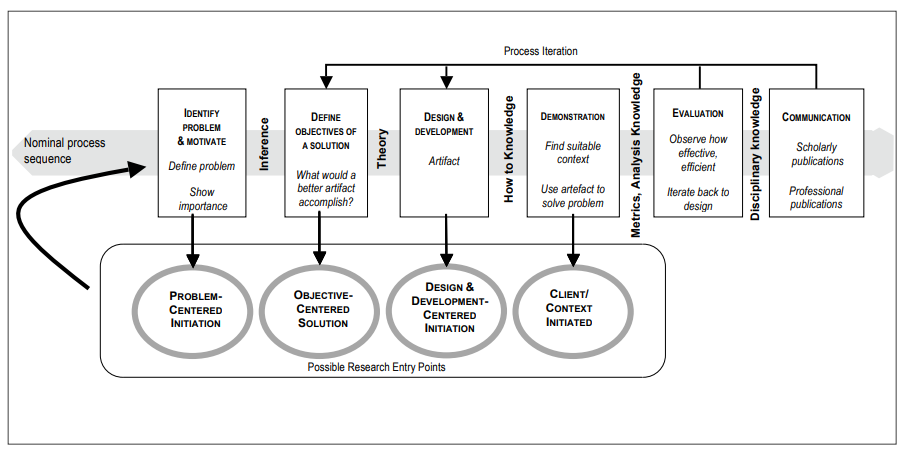
\includegraphics[width=\linewidth,height=\textheight,keepaspectratio]{Resources/DS_Peffers.png}
		\caption{Peffers et al.: Gestaltungsorientierte Forschung \cite{peffers_design_2007}}
	\end{center}
\end{figure}

Diese sechs Phasen können sequentiell von der ersten bis zur letzten durchgearbeitet werden, aber nicht zwangsläufig. Ein Forscher kann auch an einer für ihn passend erscheinenden Phase beginnen und von dort aus weiterarbeiten. Problemzentrierte Forschung beginnt in Phase 1, \textit{Problemidentifikation und Motivation}. Dieser Ansatz wird häufig gewählt, wenn auf früherer Forschung aufgebaut oder von der Beobachtung eines Problems begonnen wird. Zielorientierte Forschung hingegen startet meistens in Phase 2, \textit{Ziel der Lösung}. Dies wird oft durch einen Anstoß aus der Industrie angetrieben. Gestaltungsorientierte Ansätze beginnen mit Phase 3, \textit{Gestaltung und Entwicklung}. Dabei gehen die Forscher meist von einem unfertigen, nicht komplett durchdachten Artefakt aus früherer Forschung oder Projekten aus. Eventuell stammt das Artefakt sogar aus einer anderen Forschungsdomäne und wurde zur Lösung eines anderen Problems erstellt. Mit Phase 4, \textit{Demonstration des Artefakts} beginnt die kunden- oder kontextbasierte Forschung. Dabei entstand die Idee beim Beobachten einer praktischen Lösung, welche funktioniert. Die Forscher arbeiten dabei rückwärts und versuchen so die bestehende Lösung zu verbessern. Dieser Ansatz kann aus einer Consultingerfahrung hervorgehen.

In dieser Arbeit wird mit Phase 1 begonnen, da das Problem anfangs durch die Ethnographie identifiziert wurde. Im Folgenden wird die Methode von Peffers genauer beschrieben \cite{peffers_design_2007}.

\subsection{Problemidentifikation und Motivation}

Peffers diskutiert Ansätze verschiedener Wissenschaftler zu Problemidentifikation und wie man Ideen findet, welche umsetzenswert sind. Der Ansatz, welcher von Pfeffers aufgegriffen wird, von Archer \cite{archer_systematic_1965} und Eekels \cite{eekels_methodological_1991} bezieht sich auf angewandte Probleme, also welche die bei einer Tätigkeit auffallen, auftreten und behindern. \\
In diesem Abschnitt muss die Suche nach einer Lösung für ein Problem begründet werden. Der zu betrachtende Umstand wird dafür genau dargelegt und definiert. Das Problem wird in kleine Teile gespalten und genau beleuchtet. Durch eingehende Betrachtung kleiner Teilbereiche kann die Komplexität des Problems in der Lösung abgebildet werden. Nur aus einer ausreichenden Problembeschreibung lässt sich ein fundiertes Artefakt erzeugen. 

Aus der Motivation ergeben sich zwei Vorteile für den Forscher: \\
Das Problem zu identifizieren und so die Suche nach einer Lösung zu begründen motiviert den Forscher, sowie die Leser seiner Arbeit bei der Suche und der Akzeptanz der Ergebnisse. \\
Zusätzlich hilft es Lesern seine Schlussfolgerungen nachzuvollziehen. \\
Um diesen Schritt durchzuführen stehen das Wissen über den aktuellen Stand des Problems, sowie die Wichtigkeit der Lösung als Ressourcen zur Verfügung. Daraus lassen sich die Anforderungen an eine Lösung zusammenstellen \cite{peffers_design_2007}.

\subsection{Ziel der Lösung}

Auch wenn das Problem gut spezifiziert ist, lässt es sich oft nicht direkt in Ziele übersetzen. Diese lassen sich besser über einen inkrementellen Prozess bestimmen, als direkt festlegen. Damit sollen die performance Ziele der Lösung herausgearbeitet werden. 

Grundlegend leitet man die Ziele von der Problemdefinition, sowie dem Wissen was möglich und machbar ist ab. Dabei kann das Ziel quantitativ sein, also beispielsweise Umstände darlegen, für welche die angestrebte Lösung besser ist als eine existierende. Oder es handelt sich um ein qualitatives Ziel, bei dem ein Artefakt Lösungen oder Hilfe für Probleme bereitstellt, welche über das ursprüngliche Problem hinausgehen. Besonders wichtig ist dabei, dass alle Ziele logisch aus der Problemspezifikation herleitbar sind. Als Ressource zur Herleitung der Ziele sollte der aktuelle Stand des Problems, als auch bereits verfügbarer Lösungen (falls existent), vorhanden sein und deren Zweckmäßigkeit überprüft werden.

\subsection{Gestaltung und Entwicklung}

Aus den gefundenen Problemen und Zielen wird nun ein Artefakt entwickelt. Für Peffers Gestaltungsorientierte Forschung kann man dabei nach dem Prinzip "early prototyping" vorgehen, da es sich um einen inkrementellen Prozess handelt. Alle Wissenschaftler, welche Peffers untersuchte legten den Fokus auf diese Phase.

Es wird dabei ein Artefakt erzeugt. Artefakte sind für Peffers Konstrukte, Modelle, Methoden, Instantiierungen oder "new properties of technical, social, and/or informational resources" \cite{jarvinen_action_2007}. Generell ist dabei jedes Forschungsartefakt ein Objekt, welches durch Zuhilfenahme von wissenschaftlichen Beiträgen entstanden ist. Dies beinhaltet die Funktion und die Architektur des Artefakts festzulegen und daraus dann das Artefakt zu kreieren. Dabei soll der Wissenschaftler theoretisches Wissen als Ressource nutzen, welches in der Lösung zum tragen kommen soll.

\subsection{Demonstration des Artefakts}

Um die Funktionstauglichkeit des Artefakts zu testen wird es vorgezeigt. Dabei kann entweder ein Test stattfinden, um zu zeigen, dass die Idee funktioniert, oder mehrere Tests, um eine genauere Evaluation durchzuführen.

Das Artefakt wird dabei so vorgeführt, damit deutlich wird, dass es eins oder mehr der anfangs definierten Probleme lösen kann. Dazu zählt die Verwendung des Artefakts in Experimenten, Simulationen, Case Studies, Beweisen oder anderen geeigneten Aktivitäten. Als Ressource zum Durchführen der Demonstrationsphase gilt das Wissen, wie man das Artefakt einsetzen muss, um ein Problem zu lösen.

\subsection{Evaluation}

Das Artefakt wurde untersucht und nun müssen die Informationen verwertet werden. Dazu ist wichtig, dass vor der Demonstration Werte festgelegt werden, welche dabei erfasst werden. Der Wissenschaftler muss genau beobachten und messen, wie gut das Artefakt die Lösung des Problems unterstützt. Dazu vergleicht er die Ziele der Lösung mit den tatsächlich beobachteten Ergebnissen der Demonstration des Artefakts. Um dies erfolgversprechend durchzuführen, wird ein Wissen über relevante Metriken und Analysetechniken verlangt.

Der Charakter der Forschung entscheidet dabei, welche Form der Evaluation durchgeführt wird. Dabei werden Methoden verwendet, wie beispielsweise das Vergleichen der Artefaktfunktionalität mit den Zielen der Lösung aus Phase 2, quantitative Leistungsmesswerte, wie hergestellte Güter oder erwirtschaftetes Kapital, Ergebnisse von Zufriedenheitsumfragen, Kundenfeedback, Simulationen, oder quantifizierbare Messwerte der Systemperformanz, wie Reaktionszeit oder Verfügbarkeit des Systems. Die Evaluation kann alle möglichen geeigneten empirischen Daten oder logische Beweise enthalten.

Am Ende dieser Phase kann der Forscher entscheiden ob er wieder zu Phase 3 zurückgeht und die gewonnenen Erkenntnisse nutzt um ein neues, besseres Artefakt zu entwickeln, oder ob er in die letzte Phase der Methode fortschreitet und die weitere Entwicklung zukünftigen Projekten überlässt. Dabei gibt die Art der Forschung an, welche Methode sinnvoller ist.

\subsection{Kommunikation der Ergebnisse}

Die gewonnenen Erkenntnisse müssen nun entsprechend Kommuniziert werden, um sie zu verbreiten. Dies sollte das Problem und seine Wichtigkeit, das Artefakt und seine Nützlichkeit und Neuartigkeit, die Einzelheiten des Designs und seine Effektivität enthalten. Die Publikation sollte an andere Wissenschaftler oder relevante Gruppen, wie zum Beispiel praktizierende Personen aus dem entsprechenden Bereich gerichtet sein. 

In wissenschaftlichen Publikationen kann die Struktur dieser Methode genutzt werden, um die Ausarbeitung zu strukturieren, wie beispielsweise empirische Forschung durch den empirischen Prozess (Problemdefinition, Literaturrecherche, Aufstellen der Hypothesen, Datensammlung, Analyse, Ergebnis und Fazit) strukturiert wird. Die Kommunikation der Ergebnisse erfordert Wissen darüber, wie Arbeiten in der entsprechenden Disziplin verfasst werden. 

\section{Designen des Fragebogens}

Diese Arbeit zielt darauf ab, einen theoretischen, sowie einen praktischen Beitrag abzuleiten. Dazu wurden Anmerkungen der Testpersonen während und nach den Probandentests notiert. Diese Informationen können dazu genutzt werden, Ideen zu sammeln und die Applikation zu verbessern, allerdings lassen sie sich nicht gut vergleichen. Sie stellen den praktischen Beitrag dar. Für den theoretischen Teil benötigt man vergleichbare Werte und Größen. Dazu wurde ein Evaluationsbogen konzipiert, der folgende Fragen beantworten soll:

\begin{itemize}
	\item Wie ist der Bezug des Handwerkers zu technischen Geräten?
	\item Wie komplex ist der Umgang mit dem System?
	\item Kann der Handwerker sich vorstellen die Technologie in Zukunft zu nutzen?
\end{itemize}

Ersteres soll Helfen abzuschätzen, wie sehr die technische Versiertheit des Handwerkers sich auf die Akzeptanz bzw. das Interesse an der Applikation auswirkt. \\
Die Nutzung eines neuen Systems, in diesem Fall einer AR Anwendung, stellt für die Handwerker aus unternehmerischer Sicht eine Risiko dar. Deshalb ist es essentiell bestimmen zu können, ob die Anwendung von den Nutzern akzeptiert und genutzt werden wird. Die beiden weiteren Fragen sollen Aufschluss darüber geben, wie die Einstellung der Fachkräfte zu dieser neuen Technologie ist. Um diese Fragen zu beantworten, werden psychologisch und wirtschaftlich evaluierte Modelle verwendet. 

Um die Gebrauchstauglichkeit der Applikation zu testen, wird das \textbf{SUS} (System Usability Scale) \cite{brooke_sus_nodate} Modell verwendet. Es gibt Aufschluss darüber, wie einfach oder umständlich die Bedienung für den Handwerker war. \\
Ein System wird nicht genutzt, wenn der Nutzer die Interaktion damit als zu Anstrengend empfindet. Um herauszufinden, als wie fordernd der Handwerker die Nutzung der Applikation empfindet, wird das Modell \textbf{NASA-TLX} verwendet. \\
Zusätzlich werden noch \textbf{TAM} und \textbf{TAM2} angewandt. Diese Abkürzungen stehen für Technology Acceptance Model. Sie wurden entwickelt, um vorherzusagen, wie wahrscheinlich ein Anwender eine Technologie nutzen wird. \\
Im folgenden werden die Modelle erklärt.

\subsection{SUS}

Bei der \textbf{System Usability Scale} handelt es sich um einen einfachen, aus zehn Punkten bestehenden Fragebogen zur subjektiven Einschätzung der Gebrauchstauglichkeit eines Systems. Es ist eine \textbf{Likert Skala}, auf welcher die Zustimmung oder Ablehnung durch sieben Punkte angegeben werden kann. Sie hilft Aufschluss darauf zu geben, ob ein System benutzt werden wird, oder nicht. \\
Nach ISO 9241-11 sollte die Messung der Gebrauchstauglichkeit folgende Aspekte abdecken \cite{brooke_sus_nodate}:

\begin{itemize}
	\item \textit{Effektivität:} Die Fähigkeit des Nutzers gestellte Aufgaben mit Hilfe des Systems zu erledigen und die Qualität der Resultate.
	\item \textit{Effizienz:} Die Menge der konsumierten Ressourcen, nötig zur Erledigung der Aufgabe.
	\item \textit{Befriedigung:} Die subjektiven Reaktionen des Nutzers auf die Verwendung des Systems.
\end{itemize}

Diese Größen zieht auch der industrielle Nutzer in Betracht, wenn er über die Implementierung einer neuen Technologie in seinem Arbeitsalltag nachdenkt. Aus unternehmerischer Sicht ist es jedoch oft nicht rentabel, eine komplette Kontextanalyse durchzuführen. SUS, mit seinen zehn Fragen, liefert eine genügende Einschätzung der Abdeckung dieser Größen.

Zur Erstellung des Fragebogens wurde ein Katalog von 50 Fragen durch John Brooke und sein Team analysiert. Dabei haben sie die zehn Fragen herausgearbeitet, welche die stärksten zustimmenden bzw. ablehnenden Reaktionen bei Probanden hervorgerufen haben. Durch die erhaltenen subjektiven Antworten auf diese Fragen lässt sich abschätzen, wie viel Training und Unterstützung neue Nutzer des Systems brauchen werden, um dieses erfolgreich zu benutzen, und wie komplex es den Anwendern erscheint.

Laut John Brooke \cite{brooke_sus_nodate} sollen die Probanden den Fragebogen ausfüllen, nachdem sie das System getestet haben und bevor eine anschließende Diskussion beginnt. Dabei sollen diese ankreuzen, was ihnen ihr Gefühl nach dem Lesen der Frage sagt und nicht lang über diese nachdenken. Alle Fragen müssen dabei beantwortet werden. Sollte ein Proband auf eine Frage keine Antwort geben wollen oder können, wird das neutrale Ergebnis der Frage angekreuzt. \\
Einzelne Antworten auf Fragen sind alleine nicht aussagekräftig. Die gesamte Auswertung aller Antworten gibt jedoch einen Wert zwischen 0 und 100, welcher die generelle Gebrauchstauglichkeit der Applikation angibt.

\subsection{NASA-TLX}

Der von NASA entwickelte \textbf{Task Load Index} (NASA-TLX) ist ein weit verbreitetes Instrument zur Bestimmung der Beanspruchung eines Probanden bei einem Testszenario oder dem Testen einer Anwendung \cite{giesa_bewertung_2003}. Er wurde ausgewählt, um zu bestimmen, als wie Anstrengend Handwerker die Nutzung von Augmented Reality empfinden und ob das eine Auswirkung auf die Akzeptanz der Technologie, sowie der Anwendung hat. Dabei misst der Index die Beanspruchung in sechs Dimensionen:

\begin{itemize}
	\item Geistige Anforderungen
	\item Körperliche Anforderungen
	\item Zeitliche Anforderungen
	\item Leistung
	\item Anstrengung
	\item Frustrationsniveau
\end{itemize}

Diese lassen sich wiederum in drei Subskalen unterteilen \cite{gros_bestimmung_2004}:

\begin{itemize}
	\item Merkmale der Aufgabe: geistige, körperliche, zeitliche Anforderungen
	\item Verhaltensmerkmale: Leistung und Anstrengung
	\item Individuelle Merkmale: Frustration
\end{itemize}

Jede dieser Dimensionen wird auf einer Skala mit 20 Stufen angegeben, die jeweils von \textit{gering} bis \textit{hoch} reicht. Jede Stufe auf der Skala wird mit 5 Punkten gewichtet. Dadurch reicht jede von 0 bis 100 und gibt somit die erfahrene Belastung zu jeder Dimension in Prozent an. Zur Auswertung wird der ungewichtete NASA-TLX verwendet. Dabei werden alle Punkte zusammengezählt und durch die Anzahl der Dimensionen geteilt. Dabei erhält man wieder einen Wert zwischen 0 und 100.

Die originale Version des NASA-TLX sieht eine Gewichtung der einzelnen Dimensionen vor. Dieses Vorgehen wurde jedoch häufig kritisiert. Nygren \cite{nygren_psychometric_1991} schlägt vor ganz auf die Gewichtung zu verzichten. Pfendler \cite{pfendler_vergleichende_1991} gibt bei der deutschen Version des NASA-TLX an, dass durch Weglassen der Gewichtung des Gesamtwerts eine höhere Reliabilität erzielt werden kann. Deshalb wird auch hier auf die Gewichtung verzichtet.

Auch wenn der NASA-TLX hoch etabliert, diagnostisch und valide ist, wird doch erwähnt, dass die deutsche Version scheinbar weniger sensitiv ist als die englische \cite{horold_faktor_2015}. In dieser Arbeit wird die deutsche Version verwendet, da die App mit deutschsprachigen Probanden getestet wird. Es wird darauf vertraut, dass die Sensitivität ausreichend ist. 

Der Fragebogen wurde mit \LaTeX  aus dieser Vorlage erstellt \cite{https://doi.org/10.13140/rg.2.2.26978.79044}.

\subsection{TAM und TAM2}

Eines der am weitesten verbreiteten Modelle in der Akzeptanzforschung ist das \textbf{Technology Acceptance Model} (TAM) von Davis \cite{davis_perceived_1989}. Es ist aus der \textbf{Theory of Reasoned Action} (TRA) von Fishbein und Ajzen \cite{fishbein_belief_1975} und der darauf basierenden \textbf{Theory of Planned Behaviour} (TPB) von Ajzen \cite{ajzen_theory_1991} entstanden. Beide Modelle stammen aus der Psychologie und analysieren wie die Einstellung einer Person zu einer Handlung, sowie subjektive Normen das Verhalten dieser Person beeinflussen. TPB zieht zusätzlich den subjektiven Aufwand, zum bewältigen einer Handlung in Erwägung und erweitert so TRA. 

Davis schlug das TAM 1989 in seiner Dissertationsschrift vor. Es bietet, vor allem im industriellen Bereich, auf Basis der Nutzungsintention eine Möglichkeit die Akzeptanz einer nicht marktreifen Technologie zu prognostizieren \cite{wilhelm_nutzerakzeptanz_nodate}. Dabei kombiniert das TAM die Größen \textit{wahrgenommener Nutzen} und \textit{wahrgenommene Einfachheit der Nutzung}, um diese Aussagen zu treffen. Ersteres gibt an, ob der Nutzer sich eine Steigerung seiner Produktivität aus der Verwendung der Technologie verspricht. Zweiteres beschreibt für wie komplex der Nutzer die Anwendung der Technologie hält. Laut Davis bewegen diese beiden Faktoren Unternehmer dazu die Technologie zu verwenden und Mitarbeiter im Umgang damit zu schulen. Das TAM bietet zusätzlich eine hohe Flexibilität, wurde in zahlreichen Studien getestet und seine Aussagekraft bestätigt \cite{university_of_arkansas_dead_2007}.

Davis erweiterte sein Modell auf die Version TAM2, um mehr auf die wahrgenommene Nützlichkeit einzugehen. Seiner Meinung nach gibt diese Determinante großen Aufschluss über die Intention eines Nutzers, wurde aber bis zu dem Zeitpunkt nicht eindringlich betrachtet \cite{venkatesh_model_1996}. Dazu ergänzte er Einflussfaktoren auf das Konstrukt wahrgenommene Nützlichkeit um \textbf{soziale} und \textbf{-	Kognitiv-instrumentelle Prozessvariablen}, sowie Betrachtungen zu unterschiedlichen Messzeiten. Soziale Variablen beschreiben dabei den Einfluss der Umgebung einer Person auf ihr Verhalten. Also wie sieht das Umfeld der Person die getestete Technologie und welchen Einfluss hat das auf die Entscheidung der Testperson. Zweitere Variable gibt wiederum an wie relevant das Ergebnis durch die Nutzung der Technologie für die Arbeit des Nutzers ist und wie gut es sich präsentieren lässt \cite{venkatesh_theoretical_2000}. Studien belegen, dass soziale Prozessvariablen anfangs die wahrgenomme Nützlichkeit für Nutzer stark beeinflussen, dies jedoch abnimmt, sobald der Proband mehr Erfahrung gesammelt hat \cite{galli_technologieakzeptanz_2016}.

\begin{figure}[h]
\begin{center}
\noindent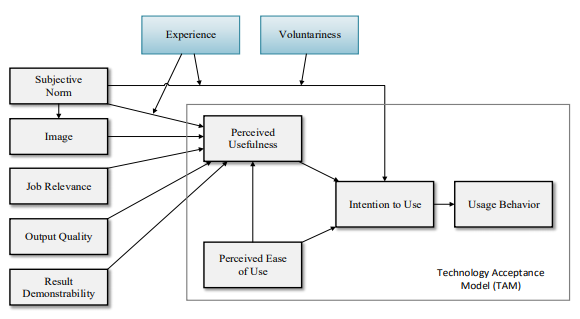
\includegraphics[width=\linewidth,height=\textheight,keepaspectratio]{Resources/TAM.png}
\caption{Technology Acceptance Modell}
\end{center}
\end{figure}




\chapter{Fokusgruppe}

In dieser Fokusgruppe wurde untersucht, wie Datenbrillen von Handwerkern aufgenommen werden und ob diese sich Szenarien vorstellen können, in welchen der Einsatz von Datenbrillen in ihrem Arbeitsumfeld hilfreich ist. Die Ursprüngliche Idee war dabei, dass Datenbrillen zur Unterstützung von Handwerkern eingesetzt werden, beispielsweise in Fernwartungsszenarien, wenn eine Person sehen möchte, was eine andere Person sieht, sich diese aber nicht am selben Ort befinden. Dann kann das Bild von der Brille des einen, zum Monitor des anderen übertragen werden. \\
Im Folgenden werden dazu die Rahmenbedingungen und die Intention, die Durchführung, sowie die Auswertung der geäußerten Ideen beschrieben. Dabei kristallisierten sich zwei Anwendungsbereiche für AR heraus, die genauer beleuchtet werden, da sie zum weiteren Verlauf dieser Forschung beitragen.

\section{Rahmen}

Um ein generelles Bild der Akzeptanz von Augmented Reality im Handwerk zu prüfen, wurde eine Fokusgruppe dazu in der Handwerkskammer München organisiert. Dazu wurden ca. 20 Handwerker aus verschiedenen handwerklichen Branchen eingeladen, um über das Thema zu diskutieren. Anfangs hielt der Moderator einen Vortrag über Augmented Reality allgemein, um den Teilnehmern die Technologie näher zu bringen. Anschließend standen verschiedene Datenbrillen, wie zum Beispiel Google Glass und die Microsoft HoloLens, zur Verfügung, welche von den Teilnehmern ausprobiert werden konnten. Die Forschungsfragen für den Workshop waren: "Was denken Handwerker über Augmented Reality, speziell Datenbrillen?" und "Können sich Handwerker Szenarien vorstellen, für welche der Einsatz von Datenbrillen für sie sinnvoll wäre?". Diese gab der Moderator den Testpersonen mit für das Testen der Brillen.

\section{Testen der Brillen}

Für jede Brille wurde eine eigene Station aufgebaut. Das Augenmerk dieser Arbeit liegt auf der Microsoft HoloLens, da dieses die am weitesten fortgeschrittene Technologie ist. Es handelt sich dabei um eine große Brille, welche mit Kameras, die ihre Umgebung filmt, sowie Mikrofon und Lautsprechern ausgestattet ist. Sie erlaubt es im Sichtfeld des Nutzers Hologramme anzuzeigen und mit diesen zu interagieren. Dieser sieht dabei die "reale Welt", welche durch die Hologramme erweitert wird. In der Fachliteratur wird dies als \textbf{Augmented Reality} oder \textbf{Mixed Reality} bezeichnet, da es reale und virtuelle Welt verschmilzt.

Das Szenario, welches mit der HoloLens nachgespielt wurde, orientierte sich an der oben genannten ursprünglichen Idee. Dies wurde mit der Applikation Skype für HoloLens und PC nachgestellt. Die Skype Applikation für HoloLens ermöglicht es dem Nutzer mit anderen über das Internet zu telefonieren. Der Nutzer sieht dabei die Webcamübertragung seines Gesprächspartners in einem Fenster-Hologramm, welches er in seiner Umgebung positionieren kann und hört diesen über die Lautsprecher der Brille. Der Nutzer am Computer sieht einen Livestream der Aufnahmen der HoloLens. Er sieht also auch Hologramme, die dieser im Raum positioniert. Beide Kommunikationspartner können mit dem Livestream und dadurch miteinander interagieren. Sie können Pfeile einzeichnen, oder Bilder in der Umgebung des HoloLensträgers platzieren. 

So ist es beispielsweise für den Brillenträger möglich dem Computernutzer ein Problem zu zeigen. Dieser kann ihn aus der Ferne beim Lösen assistieren, was in einem Laien-Experten Szenario hilfreich sein kann. Der Computernutzer erhält so einen guten Einblick in das Problem und direktes Feedback zu den Aktionen des Brillenträgers und seinen Anweisungen. Dadurch können sie sich besser abstimmen.

\section{Diskussionsrunde}

Die Diskussionsrunde wurde an einer langen Tafel abgehalten. Der Moderator stellte noch einige Applikationen und Anwendungsmöglichkeiten von Augmented Reality vor, um die Fantasie der Teilnehmer anzuregen. Danach stellte er richtungsweisende Fragen, was die Diskussion anregte. Dabei kristallisierten sich schnell zwei gefragte Themenbereiche heraus: Augmented Reality als Assistent für den Handwerker zu nutzen, der ihn bei der Ausführung seiner Arbeit unterstützt und es als visuelles Tool für das Kundengespräch zu nutzen. Die meisten Ideen drehten sich um diese Anwendungsmöglichkeiten. Zusätzlich wurde aber auch Kritik an der Microsoft HoloLens geäußert, warum sie eventuell nicht genutzt werden kann.

\subsection{Kritik an dem Einsatz von Augmented Reality und der Microsoft HoloLens}

Es wurden die hohen Anschaffungskosten kritisiert, die mit dem kauf der Microsoft HoloLens einhergehen. Diese kostet momentan ca. 3000\EURdig, was ein großer Aufwand für einen kleinen Handwerksbetrieb wäre. Dazu braucht der Handwerker auch die richtige Software, welche noch auf seine Bedürfnisse zugeschnitten werden muss. Da Teilnehmer äußerten hierzu Bedenken, dass der Kosten/Nutzen Faktor für sie nicht Interessant sein könnte.

Für das Beispiel mit Skype wurden die Bedenken geäußert, dass man dafür eine ständige, stabile Internetverbindung benötigt. Diese ist oft auf einer Baustelle oder einer großen Produktionshalle nicht gegeben. Dadurch könnten Fernwartungsapplikationen nicht verwendet werden.

Ein großer Kritikpunkt ist die Einsatzfähigkeit der HoloLens auf einer Baustelle. Dieses Umfeld ist hart, schmutzig, staubig und oft ungemütlich. Man findet schwer einen sicheren Platz zum abstellen der Brille. Bei jedem hinlegen läuft man Gefahr diese zu zerkratzen oder anderweitig zu beschädigen. Noch dazu hält sie wahrscheinlich keinen harten Stößen stand, falls sie herunterfallen sollte. Der Staub auf Baustellen kann sich negativ auf die Funktionalität der Kameras und die Darstellung der Hologramme auswirken. Gegebenenfalls erkennt die Brille dadurch die Gestensteuerung nicht mehr. Zusätzlich ist die Microsoft HoloLens ein eher unhandliches, globiges Gerät, welches man auf dem Kopf trägt. Das beeinflusst die Komfortabilität der Nutzung der Brille, vor allem bei längerem Gebrauch.

\subsection{AR als Assistent für den Handwerker}

Oft wurde von den Handwerkern der Wert einer Funktion zum automatischen Erfassen des Raumes hervorgehoben. Der initiale Prozess zum Abmessen der Wandlängen, Winkel, Einbuchtungen und sonstigem nimmt einiges an Zeit in Anspruch. Gleichzeitig handelt es sich dabei um einen wichtig Schritt, der den Grundstein für das weitere Vorgehen legt. Jeder Handwerker, sei es Fliesenleger, Maurer oder Installateur benötigt diese Daten für die Planung. Mit Augmented Reality kann es möglich sein, dies automatisch zu erfassen. Die Microsoft HoloLens beispielsweise besitzt ein integriertes \textbf{spacial mapping}, mithilfe dessen sich die Brille ein Verständnis der Umgebung verschafft. Diese Funktionalität könnte dafür genutzt werden eine solche Applikation zu integrieren. 

Nach dem erfassen des Raumes ist es für Handwerker interessant verschiedene Objekte, wie zum Beispiel Fliesen, Lampen, Fenster, Waschbecken oder ähnliches virtuell im Raum platzieren zu können. Das erleichtert die Planung, da man bereits in diesem Schritt festlegen kann, wie das Endergebnis aussieht und dadurch abschätzen kann wie viel Material benötigt wird. Das Material richtig abzuschätzen ist ein Problem, welches Handwerkern immer wieder begegnet. Zusätzlich äußerte ein Installateur die Idee, dass die Brille Verstöße gegen DIN Normen, wie beispielsweise die Höhe von Treppenstufen oder Toiletten direkt anzeigt und somit den Raum für Fehler minimiert. 

Die Datenbrille kann so also als Planungswerkzeug für den Handwerker verwendet werden. Dadurch hat er den Plan direkt vor Augen und kann ihn gegebenenfalls mit anderen Handwerkern teilen. Dies ist besonders interessant, wenn beispielsweise ein Handwerker das Kundengespräch leitet und den entstandenen Plan mit seinen Mitarbeitern teilen möchte. So kann sichergestellt werden, dass alle auf das gleiche Endergebnis hinarbeiten. Traditionell, äußerten einige Teilnehmer der Fokusgruppe, wird das oft über Telefonate abgestimmt. Dabei kommt es leicht zu Missverständnissen und somit zu Fehlern bei der Umsetzung. Eine visuelle Darstellung würde das Telefonat unterstützen und ein verständlicheres Bild zeichnen.

\subsection{AR als Assistent für das Kundengespräch}

Ein großes Problem aller Handwerker stellt das Kundengespräch dar. Sie kritisieren, dass Kunden kaum Vorstellungskraft haben. Der Handwerker kann sich das Ergebnis seiner Arbeit in einem unfertigen Raum leichter vorstellen, als der Kunde, welcher meist Laie auf dem Gebiet ist. Eine visuelle Darstellung des Plans durch Hologramme kann von diesen leichter verstanden werden, als beispielsweise ein technischer Bauplan. 

Diese visuelle Darstellung unterstützt auch beim Austausch mit dem Kunden. Dieser kann direkt sehen, wie der Handwerker seine Wünsche verstanden hat und so leichter Änderungen vorschlagen. Dadurch lassen sich Änderungswünsche, welche im späteren Verlauf der Arbeit beim Kunden auftreten könnten minimieren. Generell kann dadurch die Ambiguität in Kundengesprächen verringert werden, was eine höhere Planungssicherheit gewährleistet. 

Auch der Handwerker kann dem Kunden damit seine Vorschläge besser vor Augen führen. Die Handwerker merkten an, dass der Kunde sich oft nichts unter den Vorschlägen des Experten vorstellen kann. So werden diese ihm direkt visuell vorgeführt. Das erhöht gleichzeitig das Vertrauen in den Handwerker, da bereits beim Betrachten des Plans deutlich wird, dass DIN Normen eingehalten wurden und riskante Designs ersichtlich sind. 

Außerdem unterstützt es auch bei dem Vertragsschluss. Alle umzusetzenden Aspekte sind visuell erfassbar und dadurch digital dokumentiert. Damit lassen sich diese sehr gut im Vertrag festhalten. Es ist also für den Kunden sichergestellt, dass der Handwerker genau nach Plan vorgeht. Für den Handwerker hingegen lassen sich so Änderungen, welche vom Kunden nach der eigentlichen Vertragsschließung gefordert werden gut abgrenzen und als zusätzliche Leistungen abrechnen. 

\section{Fazit}

Ein AR Raumplaner hat, wie durch die Fokusgruppe deutlich geworden, einige Anwendungsszenarien und wird von Handwerkern gewünscht. Generell waren die Handwerker von der Technologie Augmented Reality sehr begeistert, was sich an den vielen eingebrachten Ideen zeigt. Der allgemeine Konsensus zeigt dabei auch in eine deutliche Richtung. Die ursprüngliche Idee zur Unterstützung in Fernwartungsszenarien fand nicht so viel Anklang. Handwerker interessieren sich eher für Unterstützung durch AR bei Tätigkeiten wie Maße nehmen und Planen. Auch eine visuelle Hilfe bei Kundengesprächen stellt sich als durchaus benötigt heraus. 

Allerdings wird es noch dauern, bis die Technologie ausgereift genug ist, um den Genauigkeitsansprüchen zu genügen. Die Geräte müssten für den Bau auch robuster designt und gebaut werden, um den harten Bedingungen zu trotzen. 

Zusammenfassen lässt sich jedoch sagen, dass die Datenbrillen von den Handwerkern gut akzeptiert wurden und diese Potential für die Zukunft dieser im Handwerk sehen. \\
Um diesen Ansätzen weiter nachzugehen muss tiefer in die Materie eingestiegen werden. Der Beruf eines Handwerkers muss aus der Nähe untersucht werden, um herauszufinden, wo man mit einer Applikation unterstützen kann, und ob man diese in den Arbeitsalltag eines Handwerkers integrieren kann. 

Der Beruf des Fliesenlegers würde dabei einige Aspekte abdecken. Ein Raum muss ausgemessen und darin Objekte - Fliesen - verlegt werden. Das lässt sich für Microsoft HoloLens gut umsetzen. Daher wird im nächsten Kapitel eine Ethnographie zum Beruf des Fliesenlegers angefertigt, mit dem Ziel definitive Ansatzpunkte für eine Applikation zur Unterstützung von Handwerkern, im speziellen Fliesenleger, zu erstellen.
\chapter{Ethnographie über das Handwerk des Fliesenlegers}

\section{Persönlicher Bezug}

Um meine Beobachtungen besser einordnen zu können, soll hier mein persönlicher Bezug zum Handwerk des Fliesenlegers und handwerklichen Berufen generell dargelegt werden. Ich absolvierte weder eine Ausbildung zum Fliesenleger, noch zu einem anderen handwerklichen Beruf. Meine Hobbies waren zwar bis jetzt immer im technischen Bereich angesiedelt, jedoch bezogen sie sich auf Computer und Smartphones, welche ich seit dem Start meines Studiums selbst repariere. Mit Maschinen, wie Autos oder Motorrädern beschäftigte ich mich hingegen weniger. 

Ich arbeitete nach dem Abitur als Aushilfe in einer Praktiker Filiale, wodurch ich sporadisch mit Baustoffen vertraut gemacht wurde. Diese Erfahrung half mir bei meinem Praktikum, da ich die Baustoffe kannte, mit denen wir täglich umgegangen sind und wusste wie man diese handhabt. Zusätzlich bin ich sportlich, was vorteilhaft für den körperlich anspruchsvollen Beruf eines Handwerkers ist, bei dem man oft schwer tragen muss.

In diesem Praktikum sammelte ich also meine ersten Erfahrungen in einem Handwerklichen Beruf. Ich traf den Fliesenleger bei einem Vorgespräch zum Praktikum, bei dem ich ihm meine Masterarbeit vorstellte, zum ersten Mal. Er leitet seit 25 Jahren einen Ein-Mann-Betrieb und ist in seiner Umgebung sehr bekannt und angesehen. In seiner Laufbahn erhielt er sporadisch Unterstützung durch Praktikanten oder andere Fliesenleger, arbeitete jedoch sonst allein. Er wusste also wie man mit Praktikanten umgeht und konnte mir so passend Wissen vermitteln.

\section{Ziel der Ethnographie}

Da ich nie als Fliesenleger arbeitete, sollte mir das Praktikum einen Einblick in das Handwerk geben, um Möglichkeiten zu finden, mit technischen Mitteln, die Arbeit zu erleichtern oder zu beschleunigen. Mein erstes Ziel war es, Ansatzpunkte zu finden, wo ein Fliesenleger Unterstützung brauchen kann. Also Arbeitsschritte zu identifizieren, die unnötig lang dauern, um erledigt zu werden oder umständlich sind.

Als Zweites suchte ich nach Möglichkeiten der Unterstützung, bei welchen speziell Augmented Reality nützlich sein kann. Wo also der Einsatz von AR einen Mehrwert für den Handwerker erzeugen kann.

Durch meine persönliche Mithilfe bei der Arbeit, erhielt ich einen tiefen Einblick in die Arbeit eines Fliesenlegers. Im nächsten Abschnitt erkläre ich, wie ich die erlebten Erfahrungen festgehalten habe.

\section{Durchführung der Ethnographie}

Bei meiner Beobachtung übernahm ich die Aufgabe des Praktikanten. Ich erledigte also kleinere Aufgaben, wie beispielsweise das Verfugen der Fliesen, und arbeitete dem Fliesenleger durch Tätigkeiten, wie das Tragen und Reichen der Fliesen zu. Der Fliesenleger übernahm das Legen der Fliesen selbst, weil er dies nach Augenmaß macht, dafür Erfahrung notwendig ist und dies die Qualität seiner Arbeit am meisten auszeichnet. Genauere Informationen dazu sind dem nächsten Kapitel „Ablauf und Ergebnisse der Ethnographie“ zu entnehmen.

Zur Dokumentation nutzte ich einen Notizblock, auf welchen ich meine Beobachtungen aufschrieb. Tonaufnahmen machte ich während des gesamten Praktikums keine, da diese Aufgrund der Baugeräusche unbrauchbar geworden wären und ihr Inhalt nicht viel beigetragen hätte. Ich hatte im Laufe des Tages zwischen Aufgaben Zeit oder nahm mir während kleineren Aufgaben Zeit, um Notizen zu machen. Da der Fliesenleger wusste, dass ich das Praktikum für meine Masterarbeit mache, war es kein Problem und auch für die Arbeit nicht hinderlich. Auch während der Arbeit stellte ich viele Fragen und schrieb mir die Antworten auf. Er erklärte alle Schritte, vor und während der Ausführung, damit ich die Zusammenhänge besser verstehe. Zusätzlich vervollständigte ich während den Pausen, als auch während Besorgungsfahrten in das Lager oder um Material zu kaufen, meine Notizen. Nach einem Arbeitstag bereitete ich die Informationen nach und fügte fehlende Informationen beziehungsweise Informationen, die mir erst im Nachhinein aufgefallen sind hinzu. Generell sprachen wir an den Tagen viel miteinander. Er erklärte viel von sich aus und ich stellte viele Fragen. So bekam ich ein umfangreiches Bild seiner Arbeit.

Insgesamt dauerte das Praktikum knapp zwei Wochen, vom 30.07.2018 bis zum 10.08.2018. Jeden Tag waren wir ca. von 8 Uhr bis 15 Uhr auf einer Baustelle.

Meine Aufzeichnungen fertigte ich in chronologischer Reihenfolge an. Für diese Arbeit und einen Leser ist das jedoch wenig sinnvoll die Informationen in dieser Reihenfolge aufzunehmen. Deswegen fasse ich in dieser Ethnographie die Arbeit der einzelnen Tage zusammen und gebe sie als Text, welcher den Ablauf des Fliesens eines Bades beschreibt, wieder. Die Ausführungen beginnen also beim Kundengespräch im Rohbau eines Raumes und enden in einem fertigen Badezimmer. Im Laufe meines Praktikums durchlief ich dazu alle Schritte, jedoch in unterschiedlicher Reihen-folge und auf vielen verschiedenen Baustellen. Zur Zeit des Beginns meines Praktikums bearbeitete der Fliesenleger nämlich mehrere offene Baustellen und nahm zeitgleich auch neue Projekte auf. Durch diese Anordnung der Ereignisse bekommt der Leser einen Gesamteindruck, wie die Arbeit eines Fliesenlegers aussieht und kann besser nachvollziehen wo und wie ich meine Ansätze für oben genannte Ziele fand.

\section{Ablauf und Ergebnisse der Ethnographie}

\subsection{Planung: Kundengespräch}

Ich fragte den Fliesenleger, bevor wir zur ersten Baustelle fuhren, wie Kundengespräche bei ihm normalerweise ablaufen. Dieser sagte mir, es gibt zwei Situationen:

\begin{itemize}
	\item Der Kunde hat bereits eine genaue Vorstellung, wie der Raum gefliest werden soll.
	\item Der Kunde hat keine genaue Vorstellung des Endergebnisses und verlässt sich auf die Beratung durch den Fliesenleger.
\end{itemize}

Bei ersterem hört er sich den Plan des Kunden an und bietet ihm zusätzlich beratend eigene Vorschläge an. Teilweise möchten Kunden das nicht und beharren darauf ihre Vorstellungen genau umgesetzt zu bekommen. Er persönlich führt solche Aufträge teilweise nicht durch. Dazu kommt es, wenn ein Kunde etwas umgesetzt haben möchte, was er für schlechte Praxis hält, da das die generelle Qualität seiner Arbeit schmälern und spätere Mängel auf ihn zurückfallen. 

In zweiterem Szenario legt der Fliesenleger dem Kunden seine Vorstellungen des fertigen Raumes dar. Dieser kann dann seine Meinung dazu äußern, Anregungen geben und Änderungen vorschlagen. Laut dem Fliesenleger können Kunden sich das Ergebnis aber im leeren Rohbau nicht vorstellen und überlassen ihm als Profi die komplette Planung. Eine persönliche Note im Bad zu hinterlassen und guten Kundenbezug aufzubauen sieht der Fliesenleger dabei als sein Markenzeichen.

Auf einer Baustelle arbeiten oft verschiedene Handwerker, wie Maurer, Trockenbauer, Installateur und Fliesenleger zusammen. Es ist von Vorteil, wenn sie zusammen planen, um von Anfang an festzulegen wo beispielsweise Dusche, Badewanne, Toilette und Waschbecken positioniert werden sollen. Für diese Elemente gibt es DIN Normen die eingehalten werden müssen. Eine Toilette muss zum Beispiel in einem gewissen Abstand über dem Boden aufgehängt werden. Wenn dieser Plan vorher festgelegt wird, vereinfacht das die Zusammenarbeit enorm. Auf der Baustelle auf der ich meine Beobachtungen machte, waren diese Planungen bereits abgeschlossen. Es ging also nur noch um das Vorbereiten und Verlegen der Fliesen.

Der Kunde, mit welchem wir das Kundengespräch führten war selbst Handwerker, Elektriker. Er hatte auf Baustellen schon mit Fliesenlegern zusammengearbeitet, wodurch er deren Planung und Arbeit besser einschätzen konnte. 

\begin{figure}[h]
	\begin{center}
		\noindent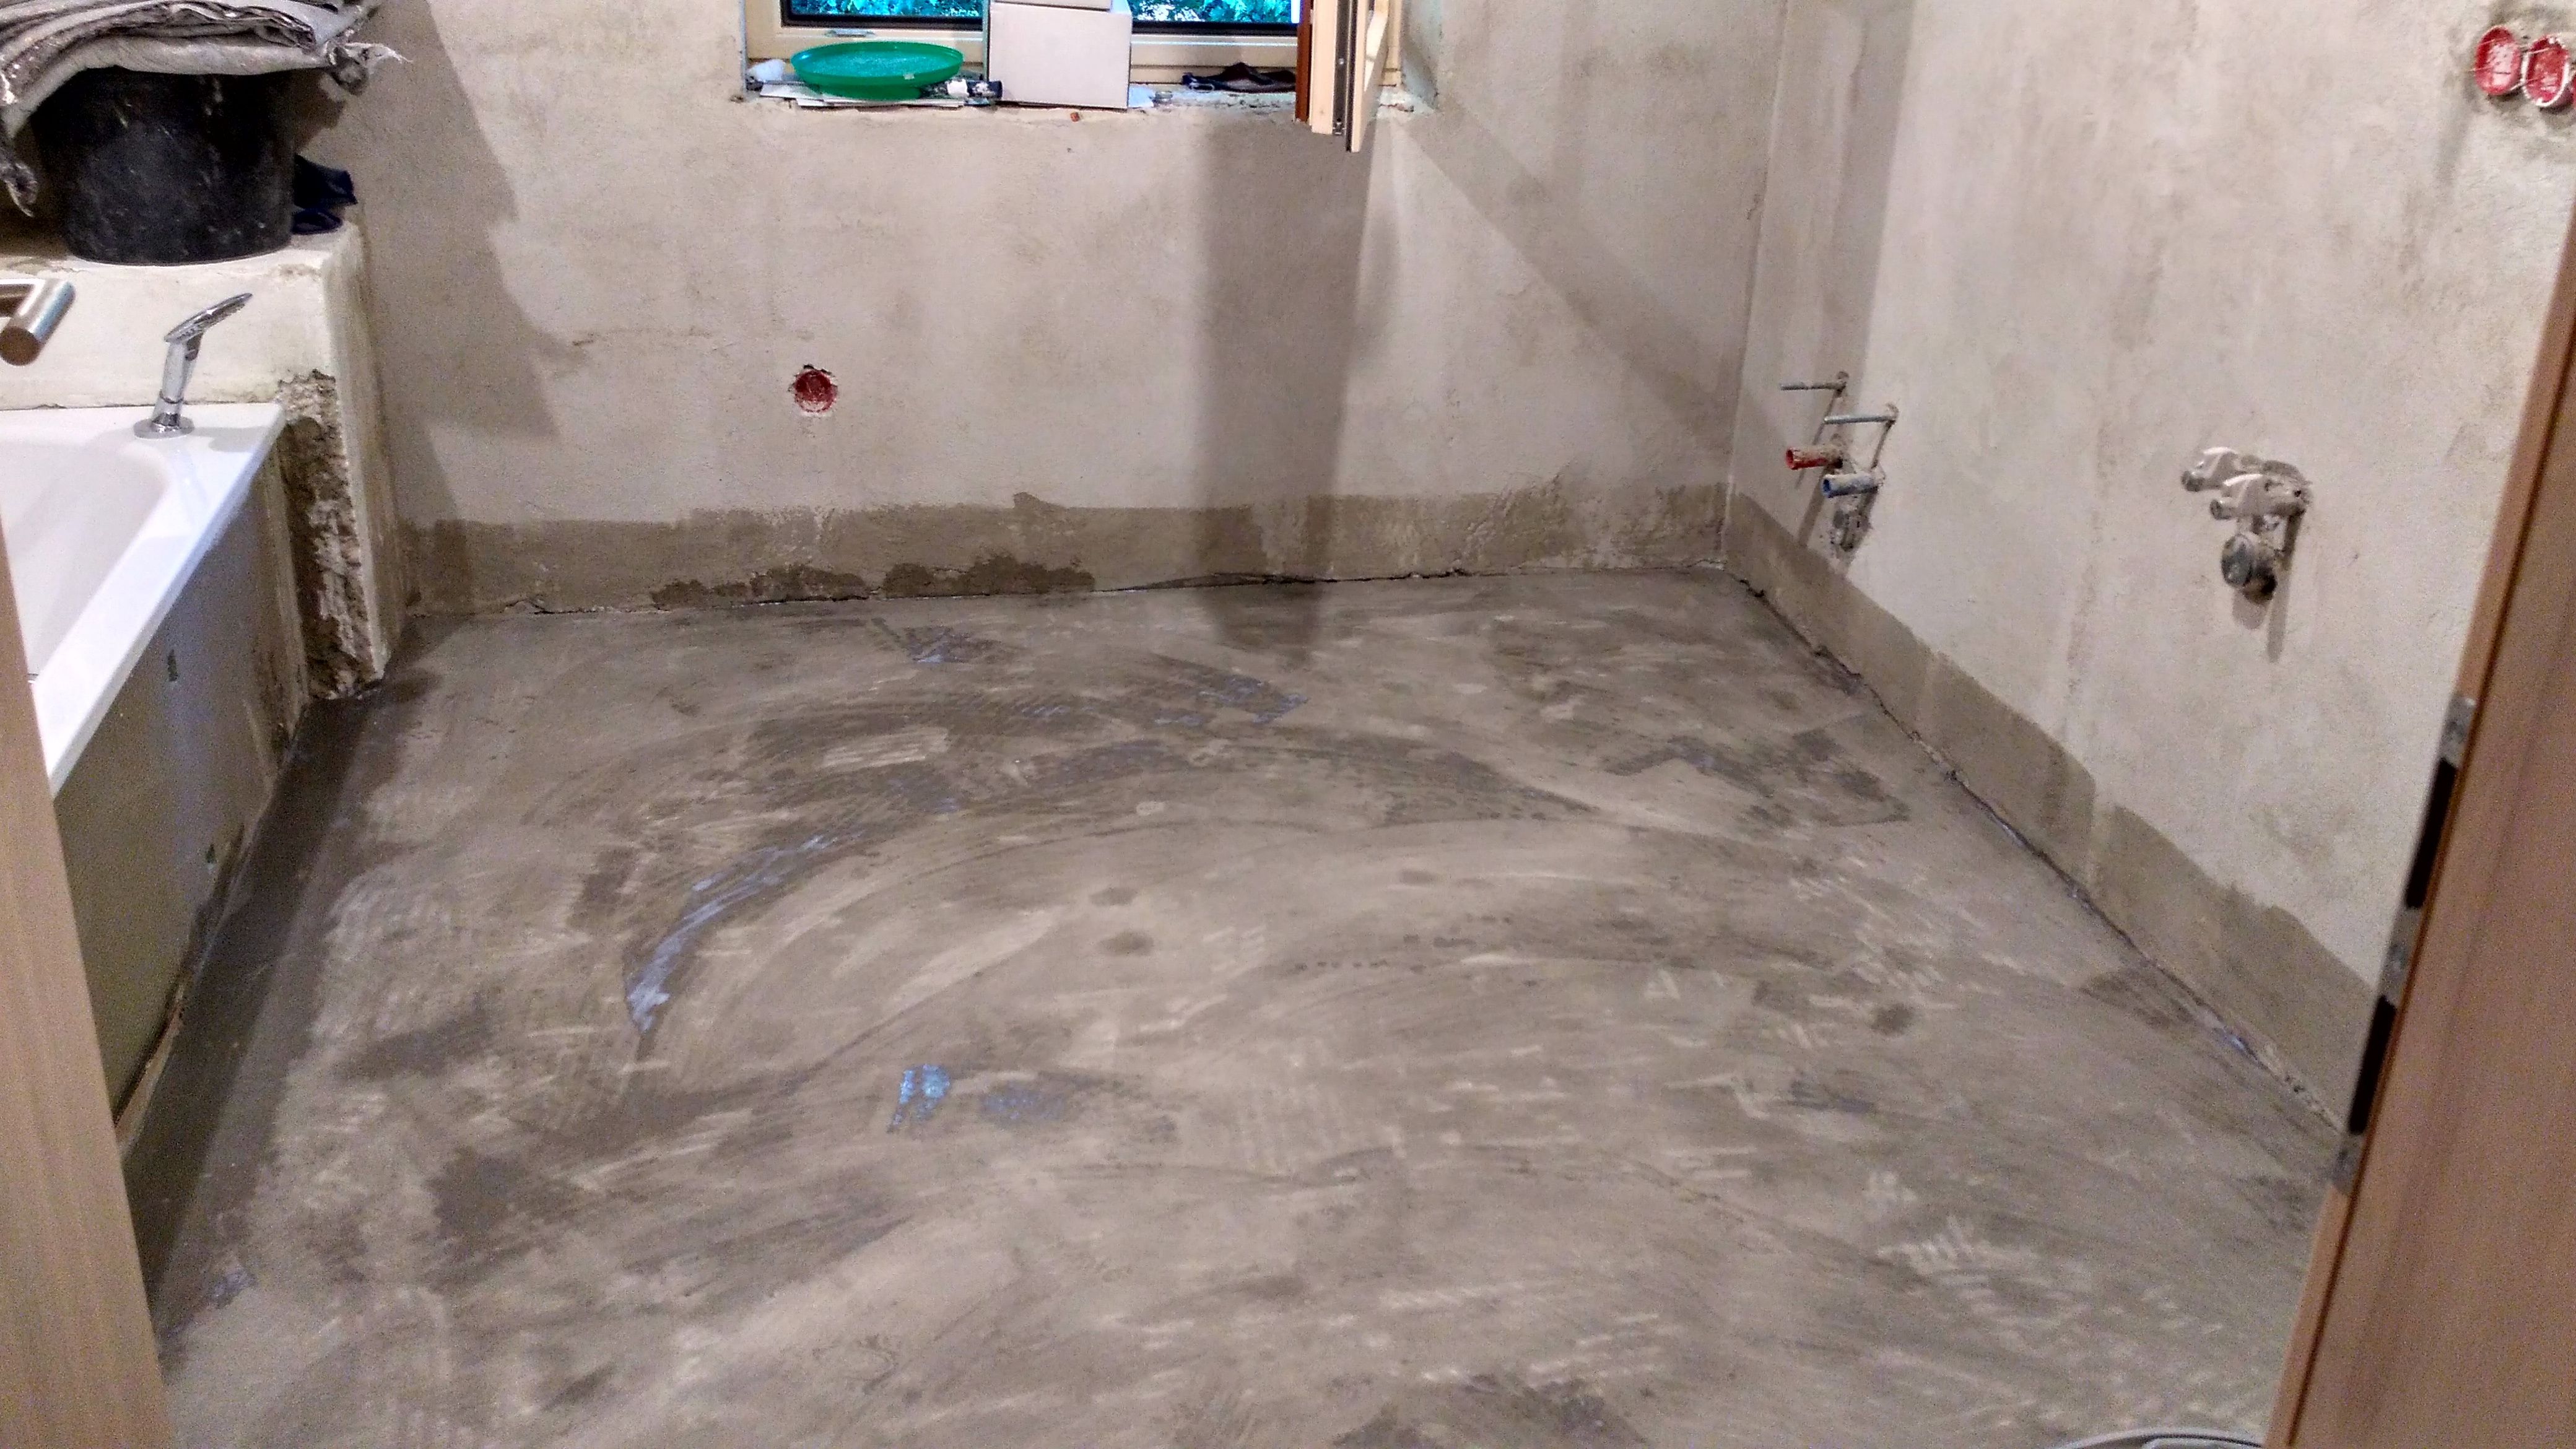
\includegraphics[scale=0.1]{Resources/Praktikum/IMG_20180801_090215_HDR.jpg}
		\caption{Rohbau}	
	\end{center}
\end{figure}

\begin{figure}[h]
	\begin{center}
		\noindent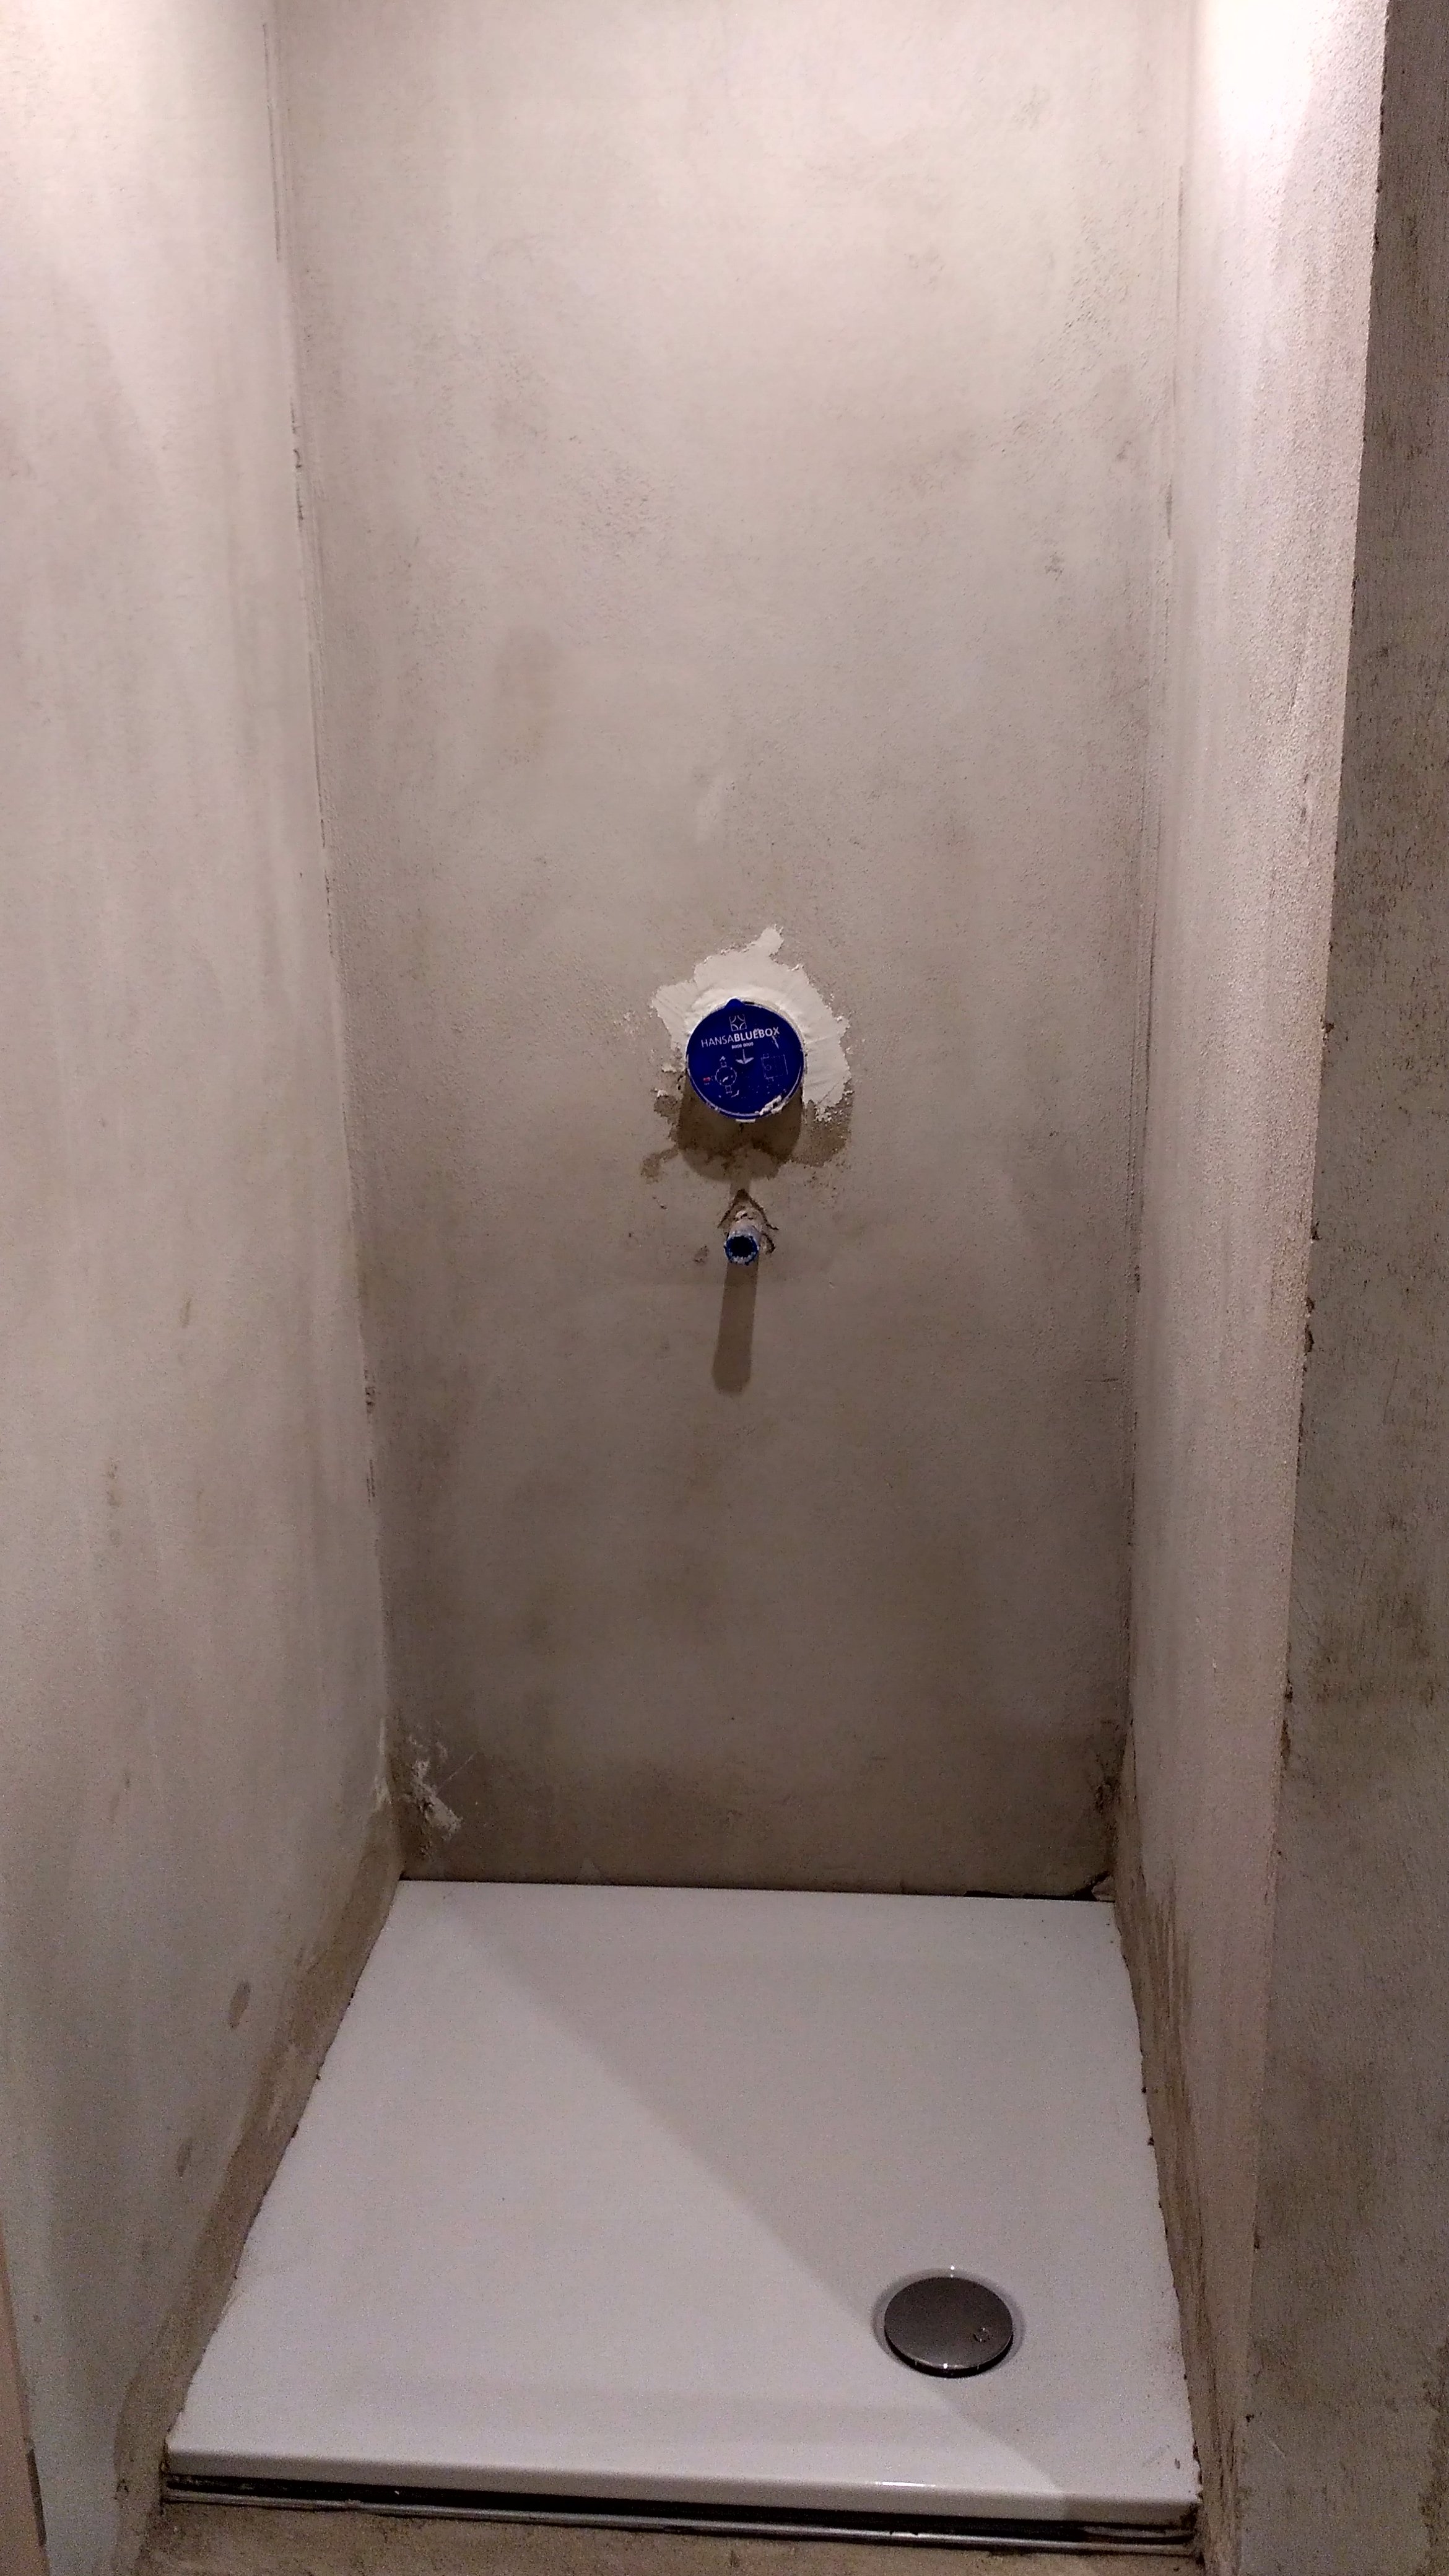
\includegraphics[scale=0.1]{Resources/Praktikum/IMG_20180731_085142_HDR.jpg}
		\caption{Rohbau: Dusche}	
	\end{center}
\end{figure}

\begin{figure}[h]
	\begin{center}
		\noindent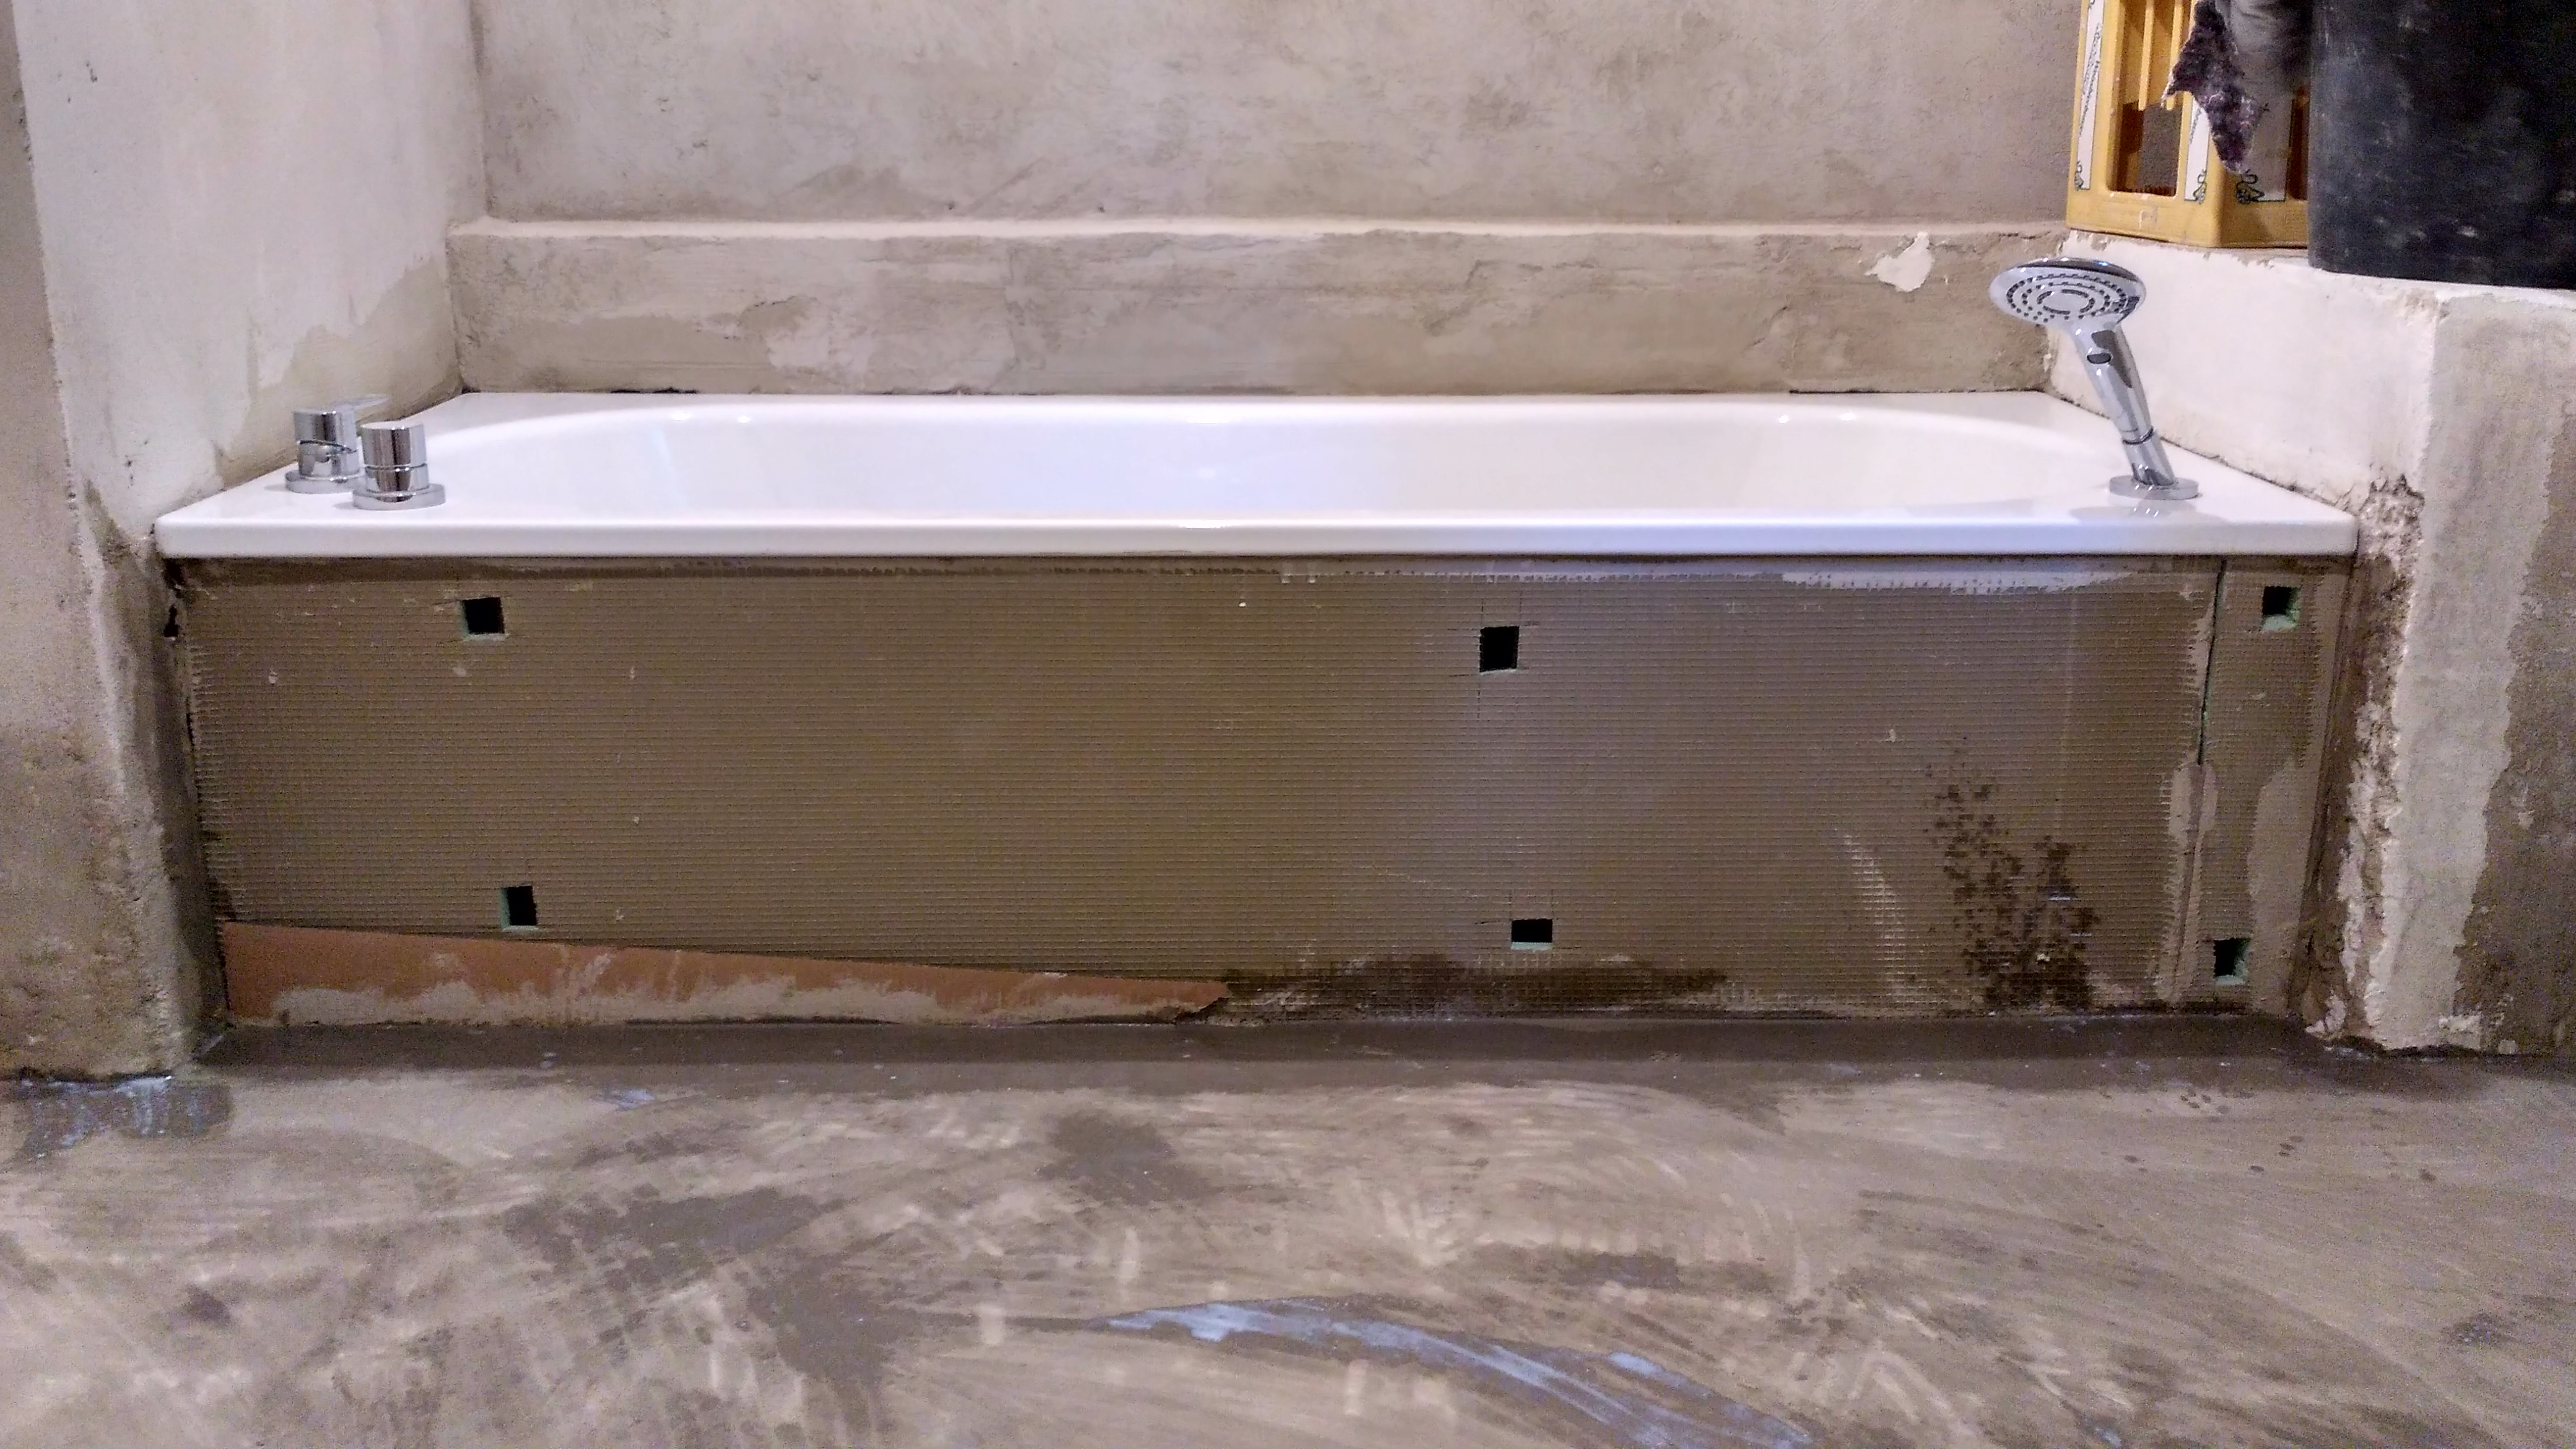
\includegraphics[scale=0.1]{Resources/Praktikum/IMG_20180801_090144_HDR.jpg}
		\caption{Rohbau: Badewanne mit eingesetzter Bauplatte}	
	\end{center}
\end{figure}

Zu Anfang führte uns der Kunde auf der Baustelle in den Rohbau des Bads, welches er verfliest und installiert haben wollte. Der Raum wurde bis jetzt nur von den Maurern verputzt. Nischen für eine Badewanne und eine Dusche waren jedoch schon vorgesehen. Die Wannen dafür waren bereits in den Nischen positioniert. Der Kunde wollte 20x30cm Fliesen im Raum verlegen, welche er uns im Katalog zeigte, und fragte den Fliesenleger nach seiner Meinung. Dieser nahm darauf seinen Meterstab zur Hand und fing an die einzelnen Seitenwände des Raumes zu bestimmen. Dies nahm ca. 5 Minuten in Anspruch. Der Fliesenleger schlug dem Kunden anschließend vor die Fliesen diagonal im Raum zu verlegen, da das ein schönes Muster ergäbe. Der Kunde reagierte auf diesen Vorschlag skeptisch und meinte er könne sich das nicht vorstellen. Er war der Meinung es sähe besser aus die Fliesen parallel zu der Wand, welche man direkt vor sich sieht wenn man den Raum betritt, zu verlegen. Der Fliesenleger skizzierte den Raum nun auf seinem Block und zeichnete die zwei Muster, parallel oder diagonal, grob ein und zeigte es dem Kunden. Die Zeichnungen verdeutlichten die beiden Ideen etwas, waren aber keine genaue Darstellung des Endergebnisses, nur eine Idee. Daraufhin begann eine rege Diskussion zwischen Fliesenleger und Kunde. Der Kunde war von seiner Idee überzeugt, stellte sich an verschiedene Punkte im Raum und schilderte seine Gedanken, woraufhin der Fliesenleger versuchte Vor- und Nachteile der Idee herauszuarbeiten. Am Ende einigten sie sich auf die Variante, die vom Kunden gewünscht wurde.

Laut dem Fliesenleger muss man die Wandfliesen an den Boden anpassen. Daher sollen auch diese horizontal zum Boden verlegt werden. Für die Wand sollen aber kleinere Fliesen verwendet werden.

\begin{figure}[h]
	\begin{center}
		\noindent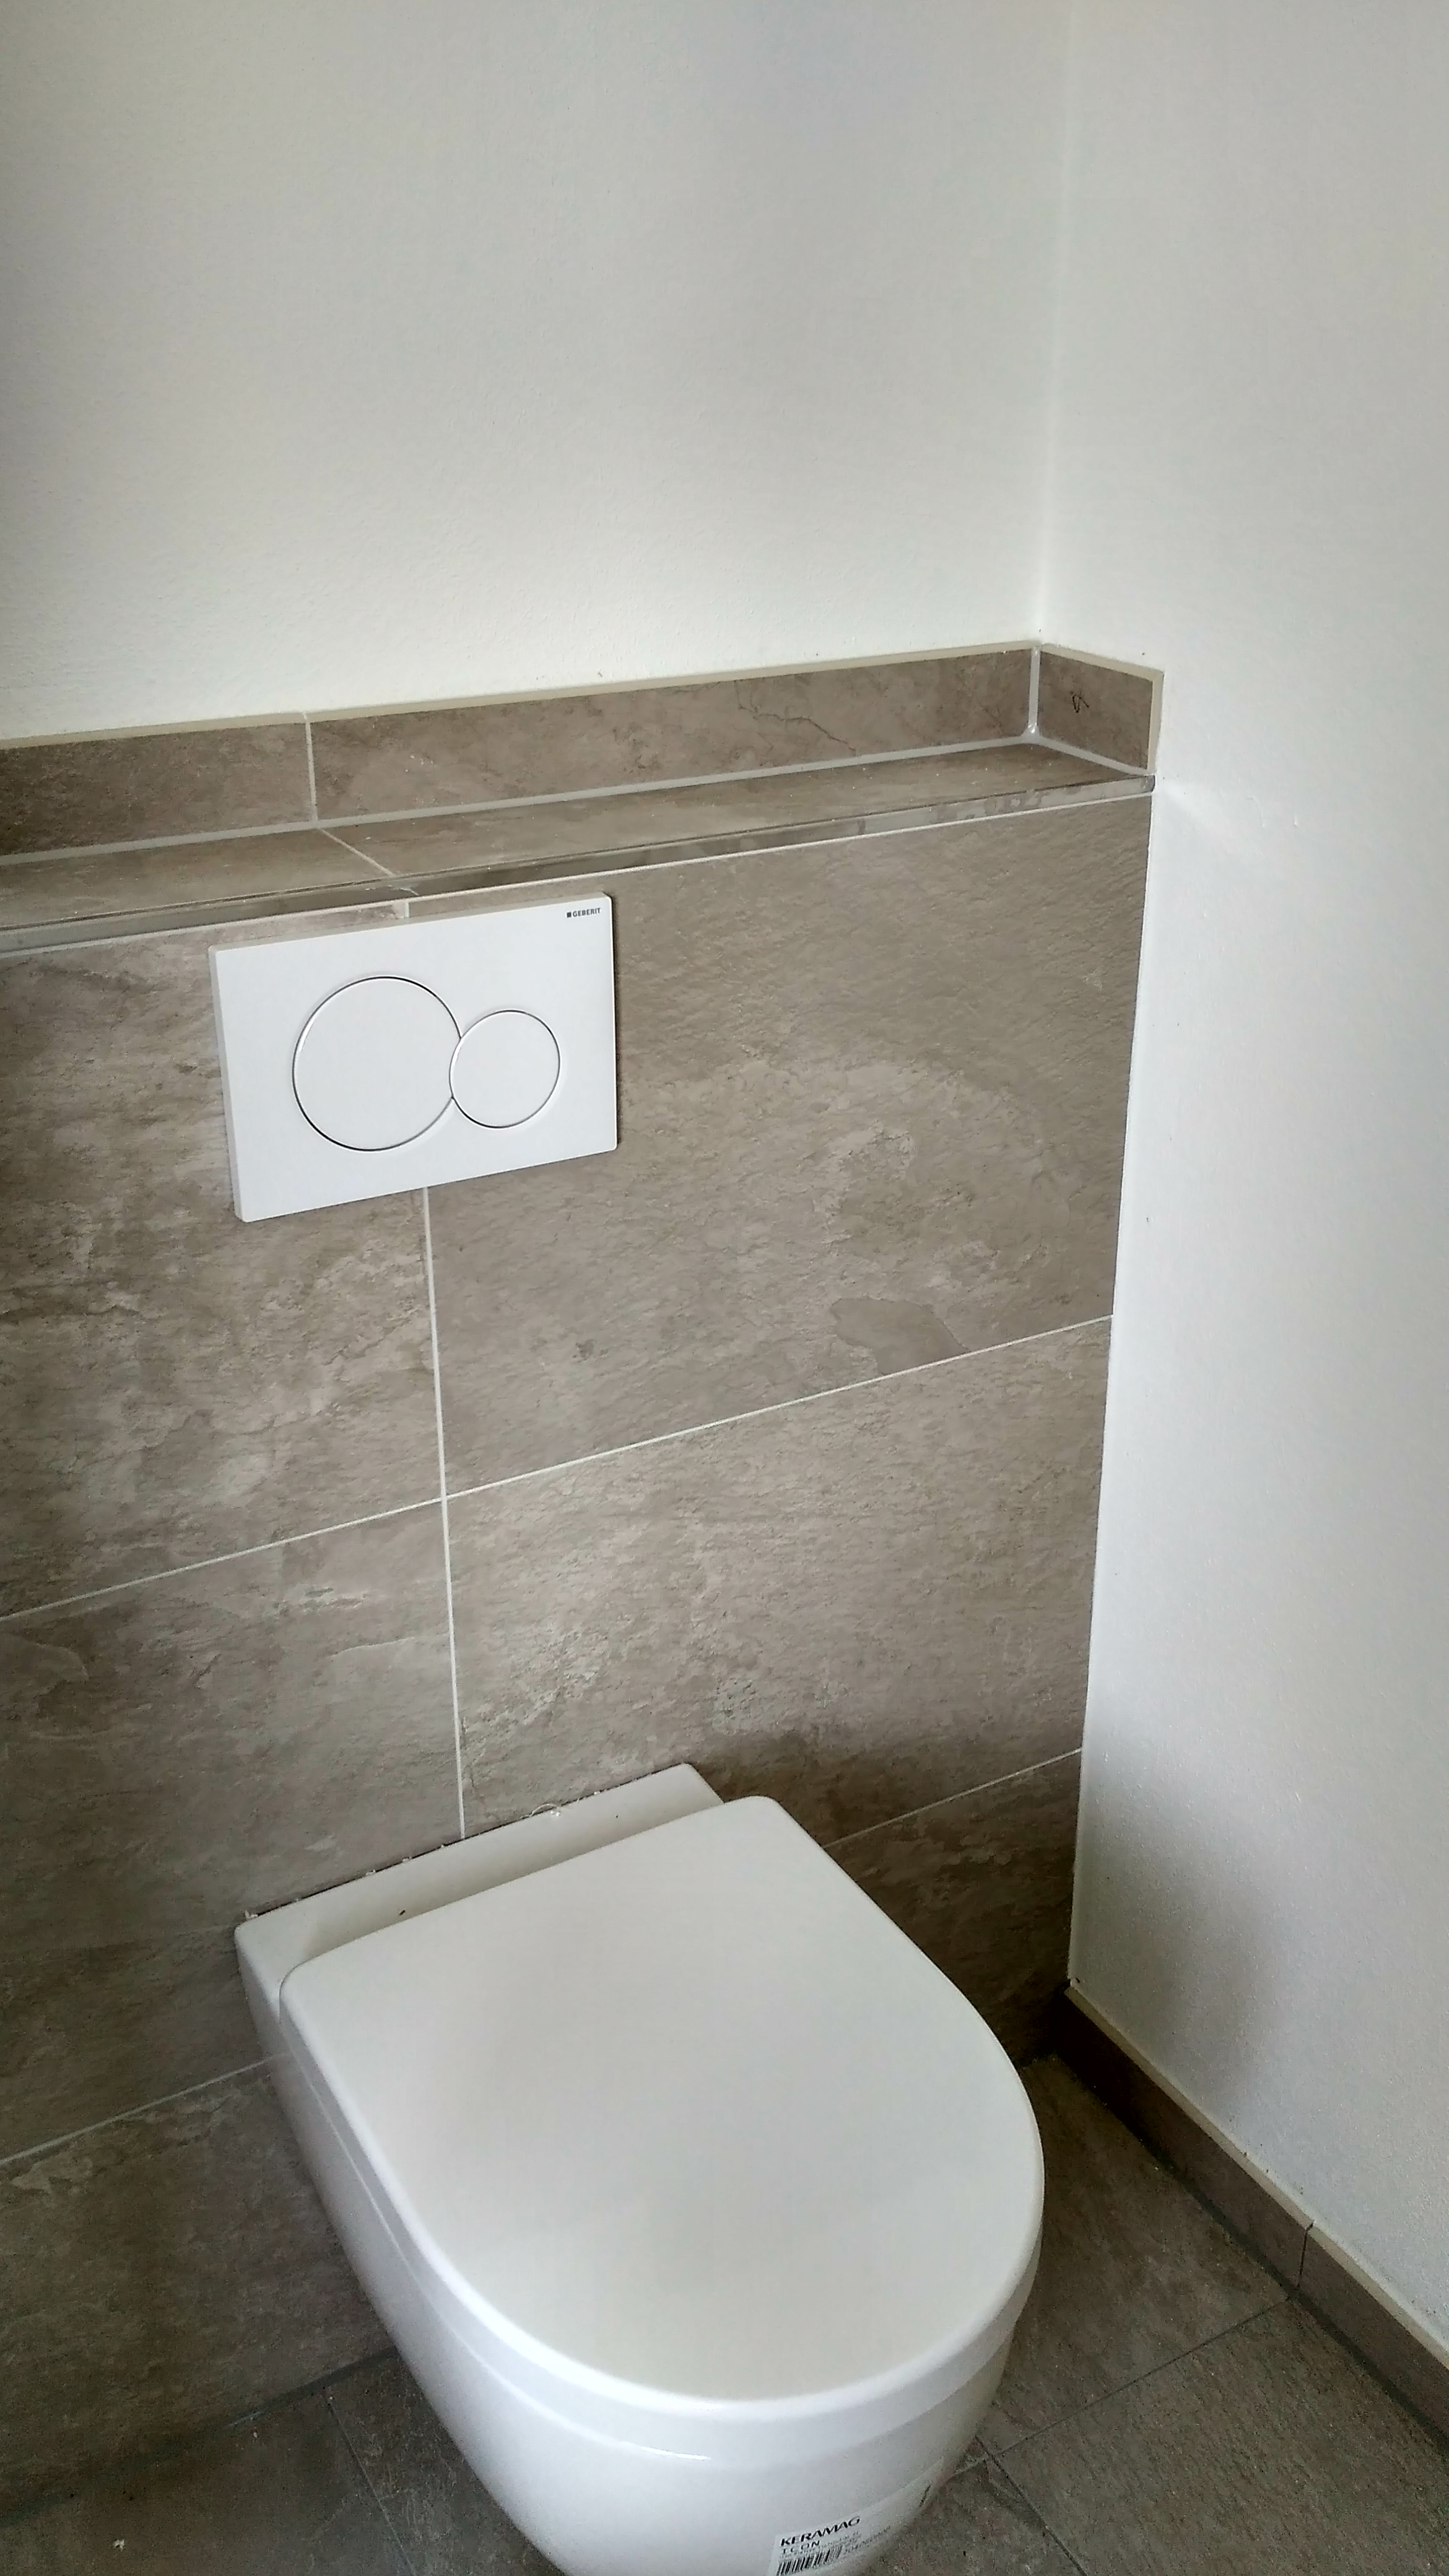
\includegraphics[scale=0.1]{Resources/Praktikum/IMG_20180801_131918_HDR.jpg}
		\label{toilette}
		\caption{Toilettenkasten mit Sockelleiste}	
	\end{center}
\end{figure}

\begin{figure}[h]
	\begin{center}
		\noindent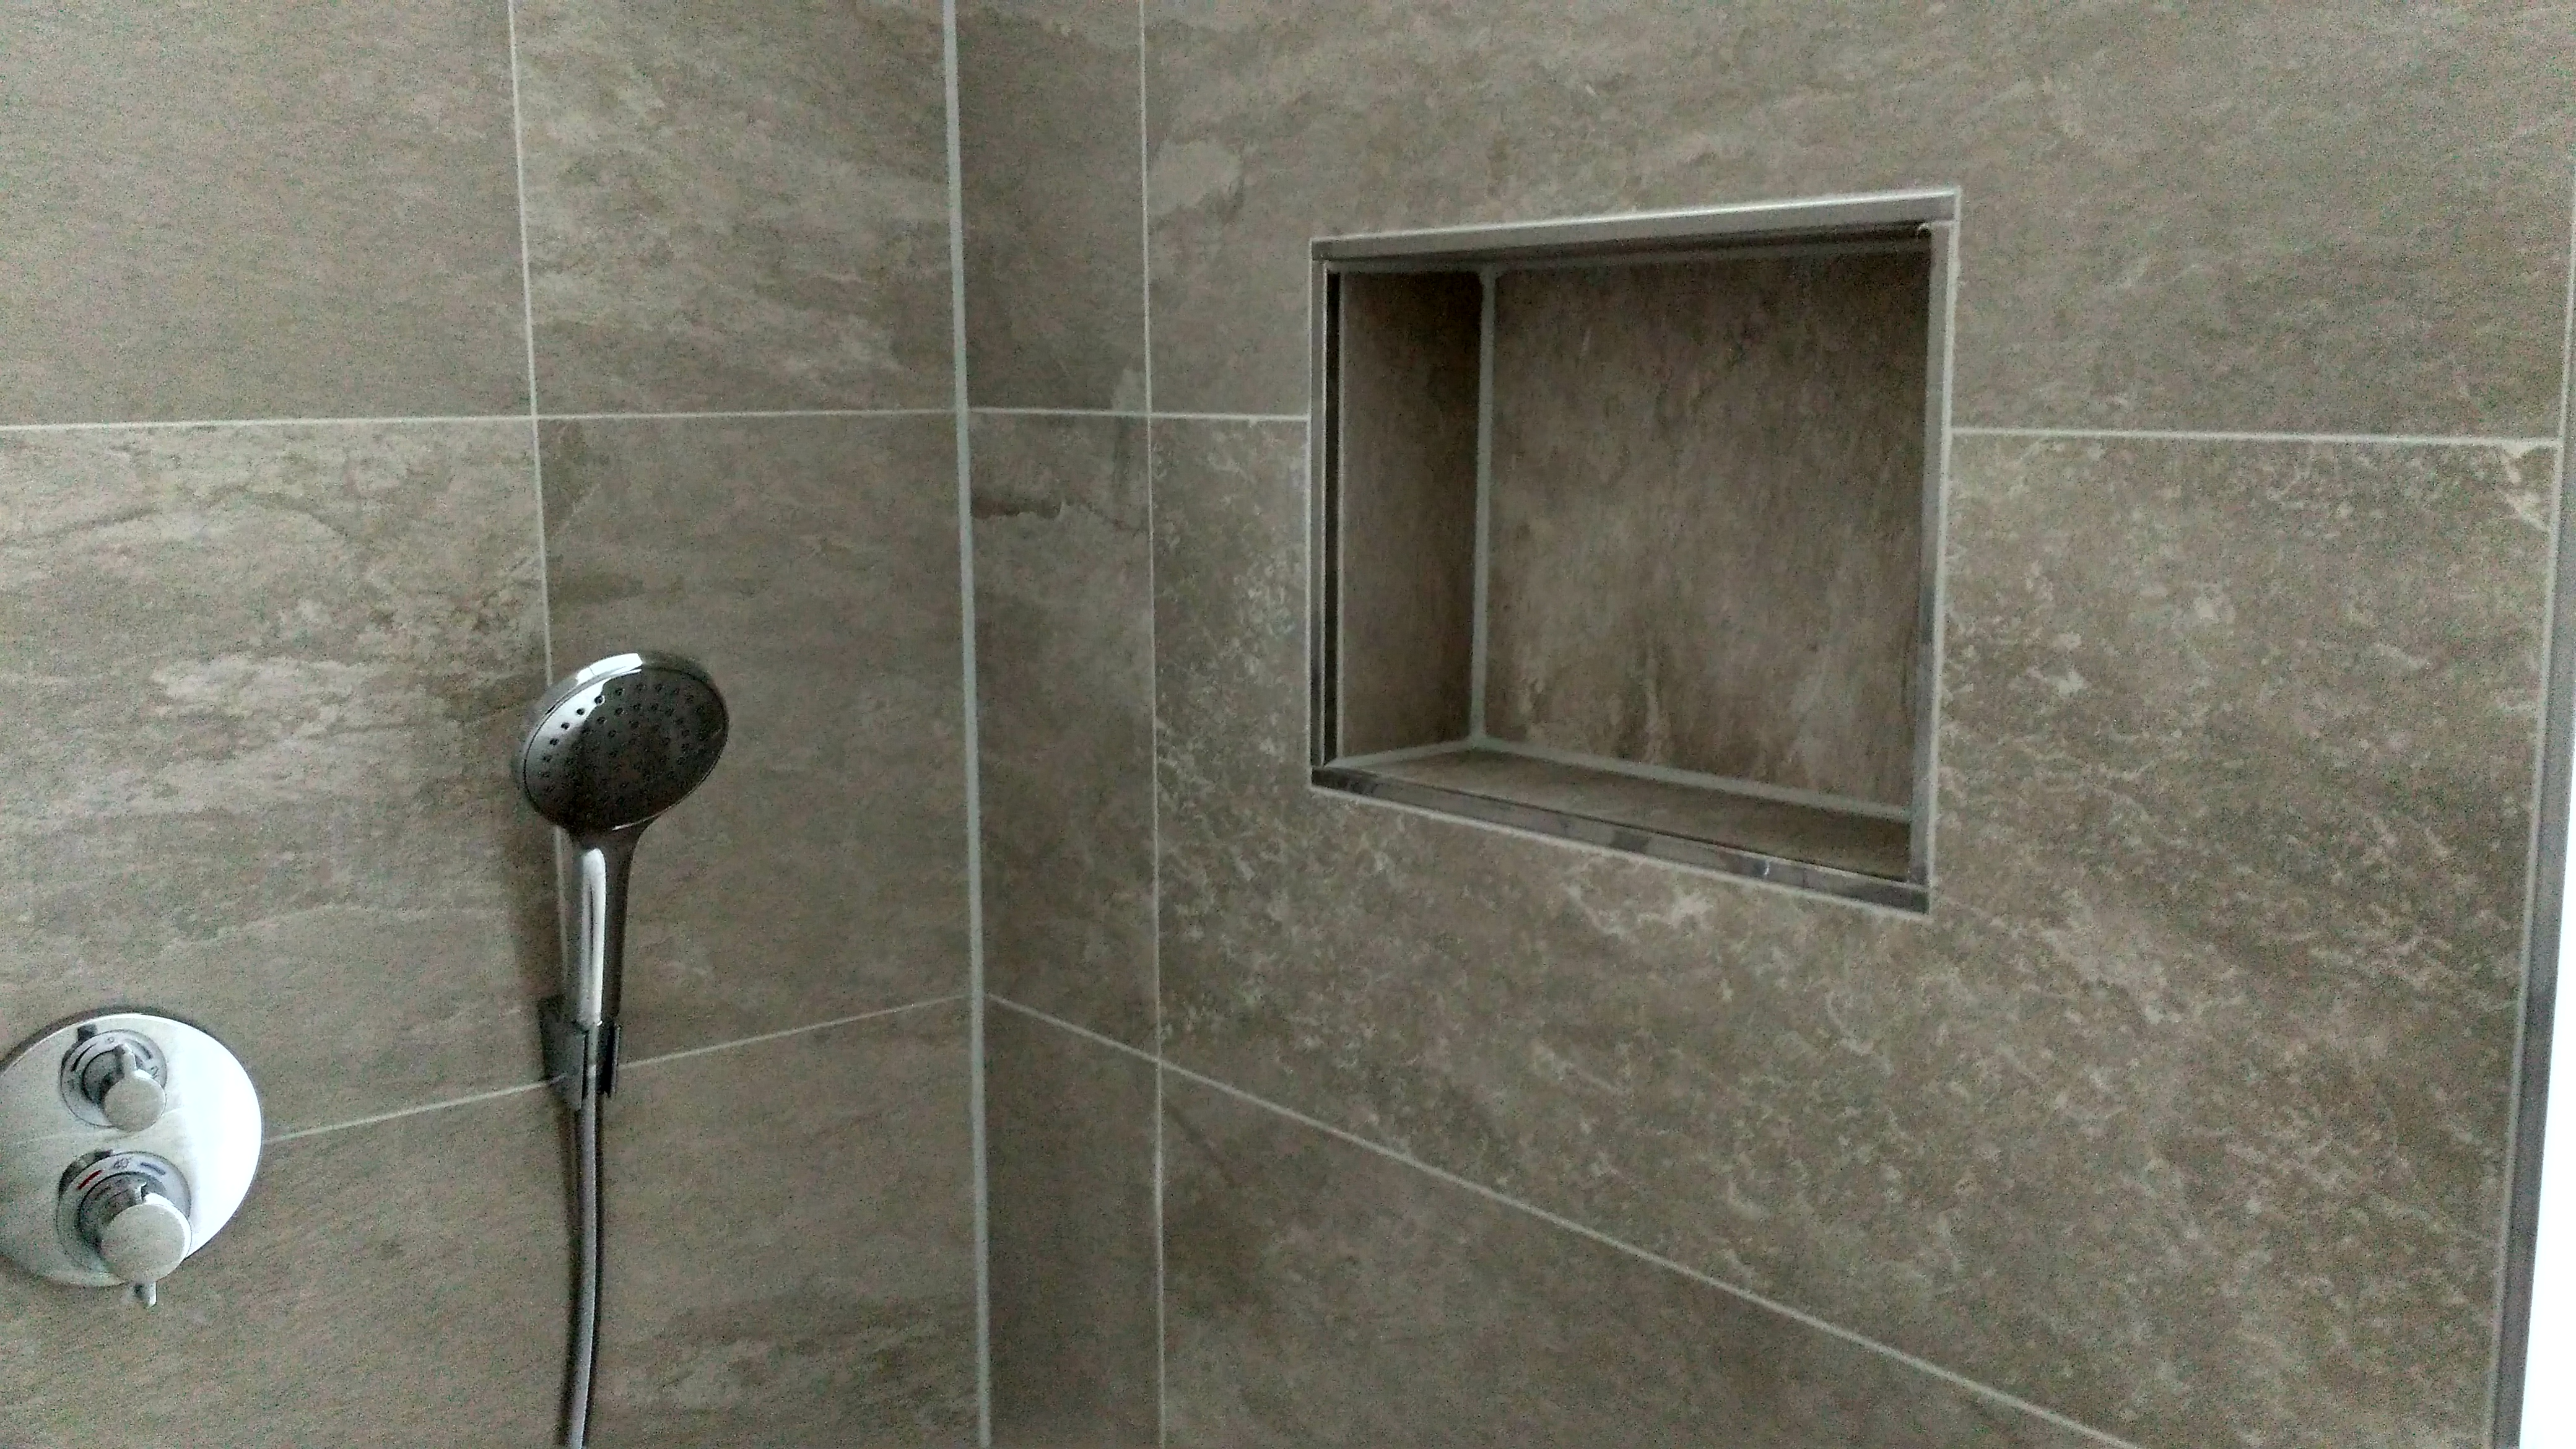
\includegraphics[scale=0.1]{Resources/Praktikum/IMG_20180801_132004_HDR.jpg}
		\label{duschenische}
		\caption{Dusche mit verfliester Abstellnische}	
	\end{center}
\end{figure}

\begin{figure}[h]
	\begin{center}
		\noindent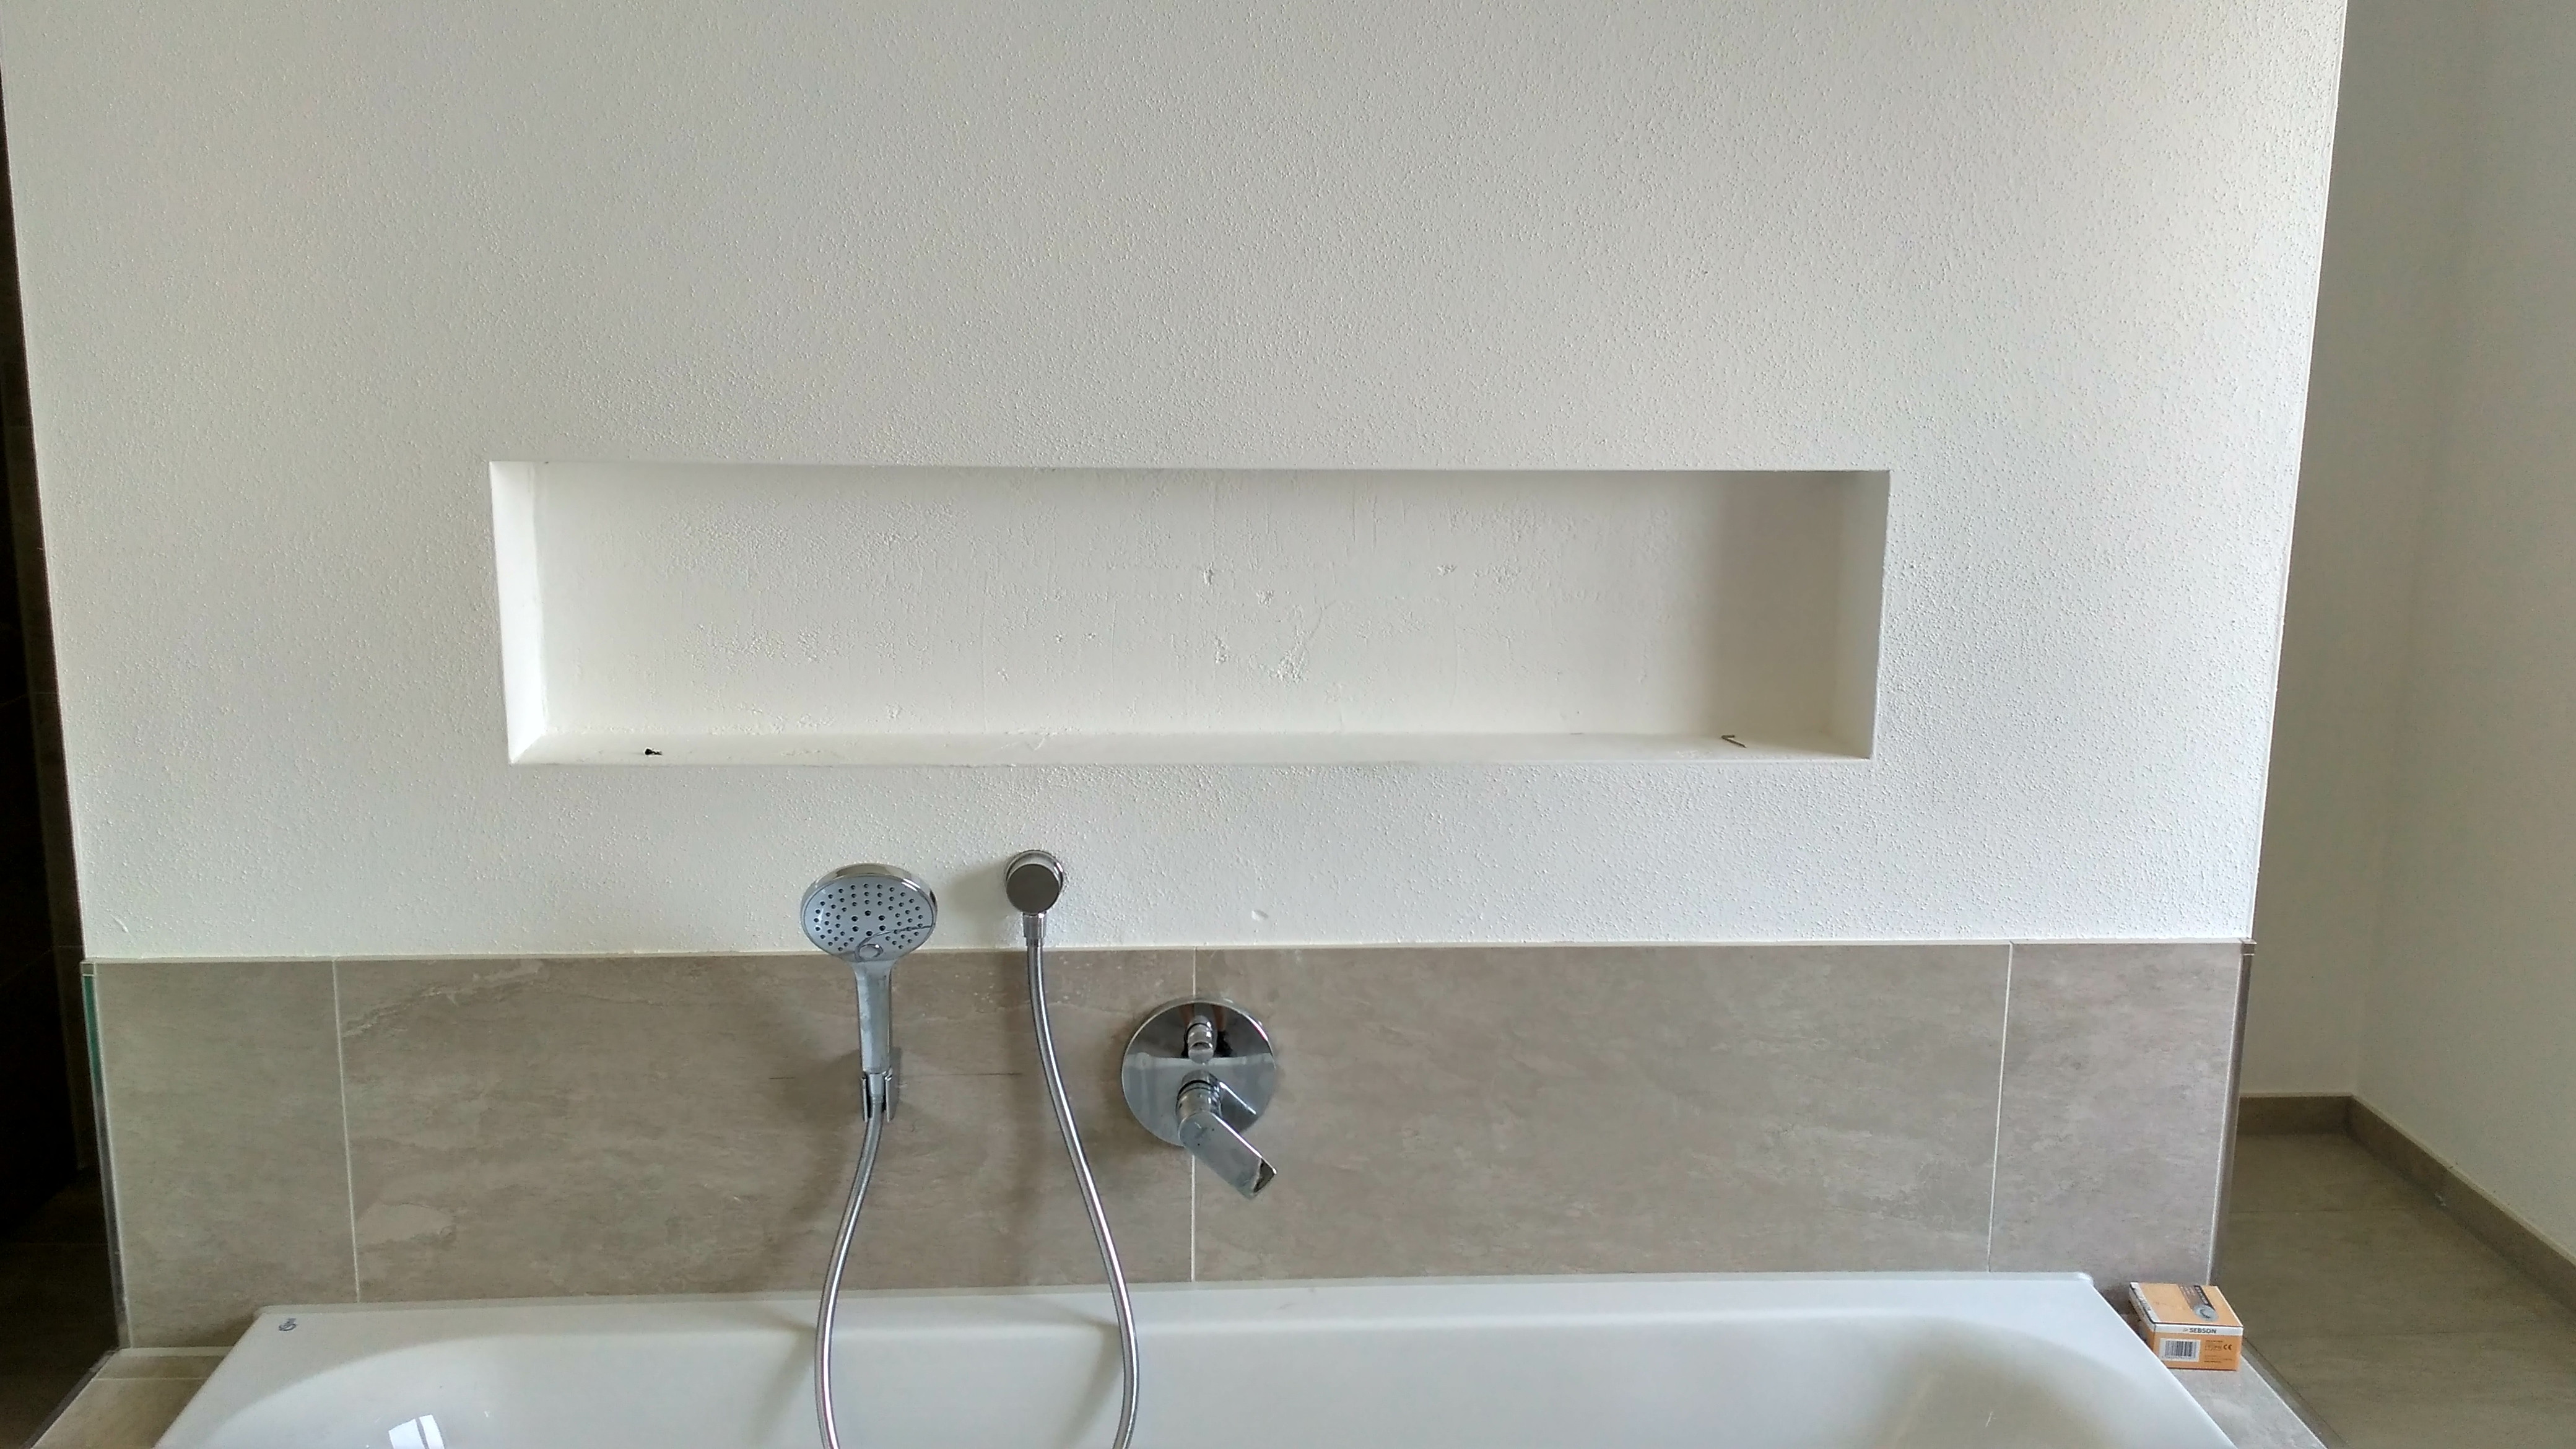
\includegraphics[scale=0.1]{Resources/Praktikum/IMG_20180801_131945_HDR.jpg}
		\label{wannenische}
		\caption{Badewanne mit nicht verfliester Abstellnische}	
	\end{center}
\end{figure}

\begin{figure}[h]
	\begin{center}
		\noindent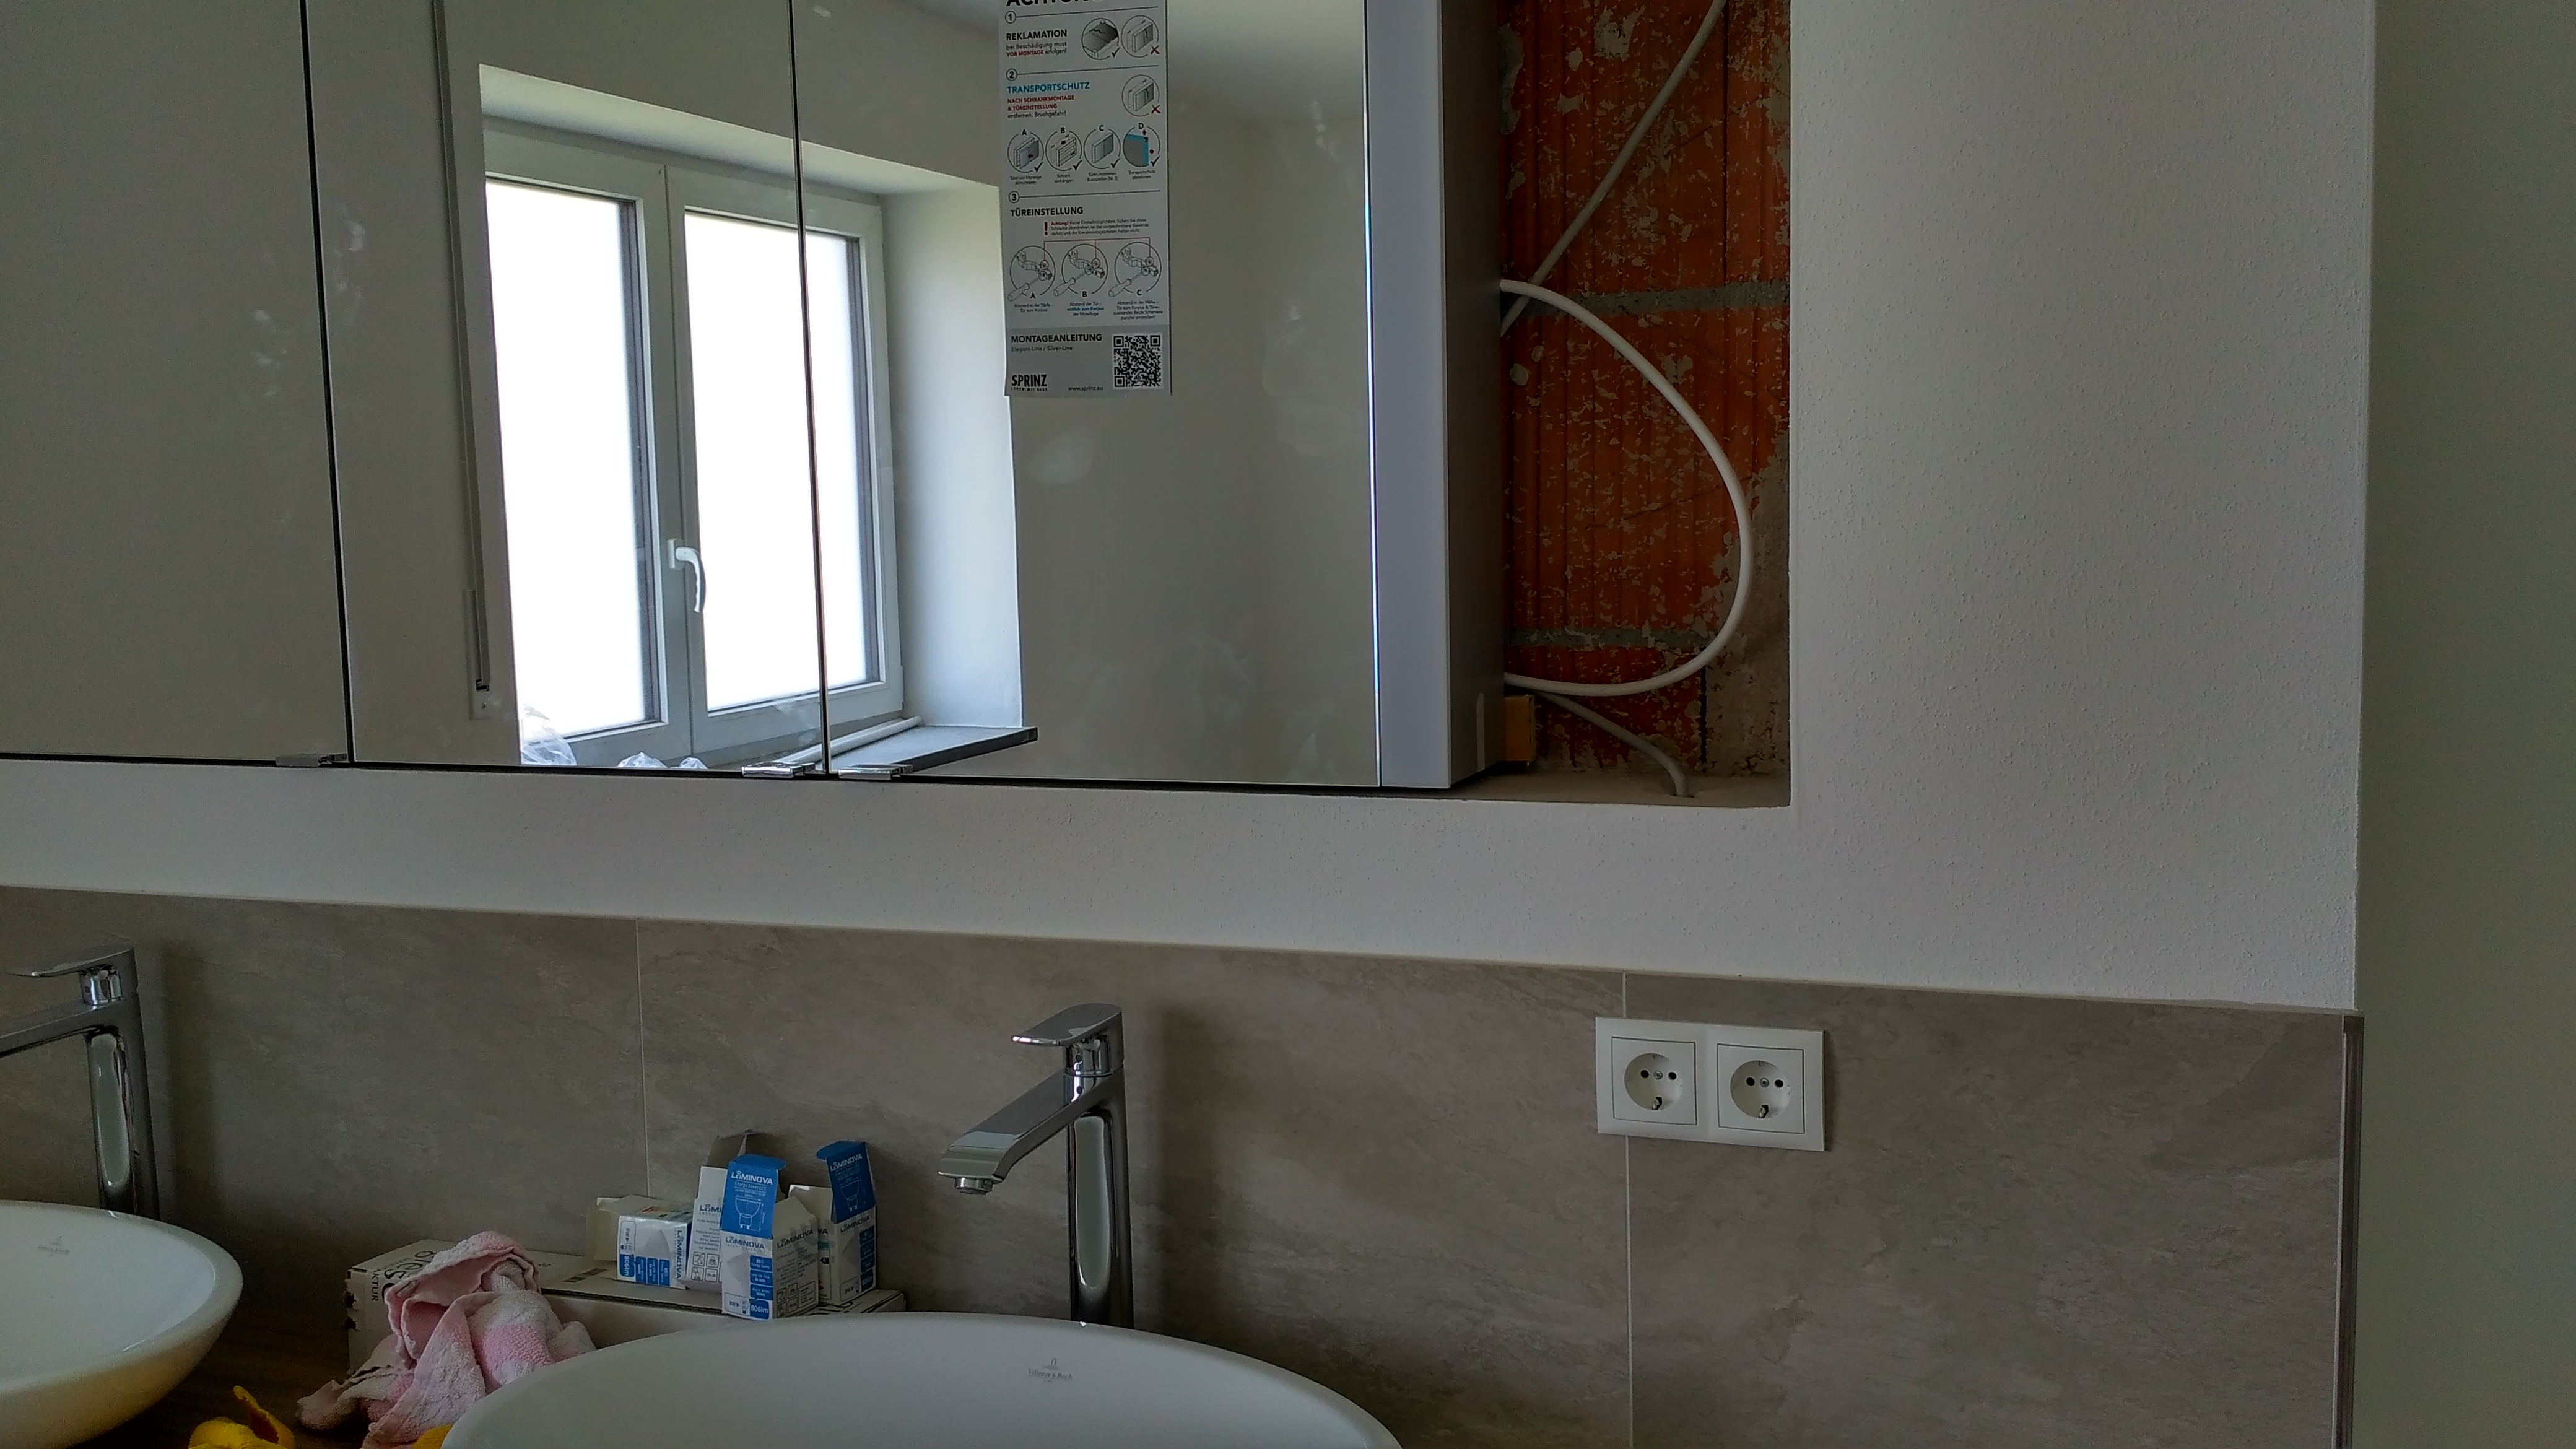
\includegraphics[scale=0.1]{Resources/Praktikum/IMG_20180801_131936_HDR.jpg}
		\label{waschbecken}
		\caption{Waschbecken mit nicht komplett verfliester Wand}	
	\end{center}
\end{figure}

Anschließend besprachen sie noch Details. Der Kunde wollte auf dem eingemauerten Spülkasten der Toilette keine Sockelleisten an der Wand anbringen. Der Fliesenleger überzeugte ihn jedoch vom Gegenteil, da sonst beim Putzen der Ablage leicht Feuchtigkeit an die verputzte Wand gelangen konnte (siehe Abbildung \ref{toilette}). Aus dem gleichen Grund riet er ihm die Nische in der Dusche, welche zum Abstellen von Duschgel gedacht ist, komplett zu verfliesen (siehe Abbildung \ref{duschenische}). Bei der Abstellnische neben der Badewanne beharrte der Kunde jedoch darauf, das diese nicht verfliest werden sollte, da es so besser aussähe (siehe Abbildung \ref{wannenische}). Er ließ sich auch von dem Argument, dass man dadurch immer Feuchtigkeit direkt auf der verputzten Mauer hat, was nicht gut ist, nicht überzeugen. Auch am Waschbecken wollte er die Wand nicht bis weit über das Waschbecken verfliest haben (siehe Abbildung \ref{waschbecken}). Dadurch entsteht die Gefahr von Feuchtigkeit auf der Wand durch Spritzwasser.

Bei diesem Kundengespräch fiel mir auf, dass es sehr unkoordiniert ablief. Die beiden Parteien redeten oft aneinander vorbei oder wiederholten ihre Gedanken, in der Hoffnung, dass ihr Gegenüber es dadurch besser versteht. Am deutlichsten wurde das bei dem Vorschlag des Fliesenlegers, die Fliesen diagonal zu verlegen. Mir kam es so vor, als könnte der Kunde sich das Muster im leeren Raum nicht vorstellen und reagierte deshalb mit Abneigung auf den Vorschlag. Ich selbst konnte es mir auch schlecht ausmalen und hätte mich hier auf den Fachmann und sein geschultes Auge verlassen müssen. Später fragte ich den Fliesenleger dazu, woraufhin er mir erklärte, dass Kunden tatsächlich wenig Vorstellungskraft besitzen, um sich komplett auf neue Vorschläge einzulassen, sich diese Vorzustellen und sie in Betracht ziehen, bei der Planung ihres Bads oder anderer Räume. Das erschwert die Kommunikation zwischen Experten und Kunden. Dadurch haben Kunde und Fliesenleger nach dem Gespräch oft unterschiedliche Vorstellungen im Kopf. Dann ist der Plan nicht genau festgelegt, was zu fehlerhafter Ausführung des Vertrags führen kann.

\subsection{Planung: Material}

Da festgelegt ist, wie die Fliesen verlegt werden sollen, geht es nun darum die Wandlängen und Winkel eindeutig zu bestimmen, festzulegen wo im Raum kritische Stellen, wie beispielsweise um ein Fenster, auftreten können, sowie wie viel Material an Fliesen, Kleber, Periplan und sonstigem gebraucht werden.

Dazu misst der Fliesenleger zuerst die Wände, um zu errechnen, wie viel Quadratmeter Bodenfläche der Raum hat. In diesem Raum, mit allen Einbuchtungen und Nischen dauerte das ca. 10 Minuten. Mit den daraus errechneten Quadratmetern kann er sich ein Bild machen, wie viel Material er zum präparieren des Bodens braucht. Da der Boden einen Riss aufweist, sollte auf diesen nicht direkt gefliest werden. Normalerweise würde man den Riss aufsägen und mit einer flexiblen Masse füllen. Unter dem verputzten Boden liegt jedoch eine Bodenheizung, welche das aufsägen zu gefährlich macht. Deshalb notiert sich der Fliesenleger auch Entkopplungsmatten für den gesamten Raum mitzubringen, welche man über den Riss legen kann, um das aufsägen zu umgehen. Zum Einmauern der Badewanne benötigt er noch eine Badewanne, wofür er sich die nötigen Maße notiert.

Der Fliesenleger erklärt mir, dass es gewisse Vorschriften für Bäder gibt, wie diese abgedichtet werden müssen. Ecken und Kanten am Boden, in der Dusche auch an der Wand, müssen mit Abdichtbändern beklebt werden. Die Wände der Dusche müssen zusätzlich noch mit Flüssigfolie ausgestrichen werden. Diese Maßnahmen dienen dazu, das Bad wasserundurchlässig zu machen und so Schimmel und ähnlichen Schäden vorzubeugen. Ein gefliester Boden gilt nicht als wasserdicht.

Aus den Quadratmetern des Raumes lässt sich leicht bestimmen, wie viele Fliesen benötigt werden. Der Fliesenleger überlegte sich, wo er mit dem Verlegen der Fliesen beginnen sollte. Dabei stellte er sich vor allem zwei Fragen:

\begin{itemize}
	\item Wie sieht das Ergebnis am besten aus?
	\item Wie minimiert man den Verschnitt?
\end{itemize}

Dazu sagte er mir, ganze Fliesen sehen am besten aus, weshalb er versucht diese im Blickfeld, beim Betreten des Raumes zu positionieren. Ganze Fliesen sehen immer ansprechender aus als geschnittene. Er maß aus, wie viele ganze Fliesen er nebeneinander legen konnte, und wie viel er von der Letzten in der Reihe abschneiden musste. Ungünstiger Verschnitt wären Fliesen von unter 1cm Breite, welchen er zu vermeiden versucht. Seine Abschätzung zeigte aber, dass die geschnittene Fliese mindestens 5cm Breit sein würde. Anschließend misst er die Winkel der Ecken genau. Haben diese nämlich keinen exakten 90 Grad Winkel, führt das später zu Ungleichmäßigkeiten am verlegten Boden, wenn er es nicht vorher entdeckt. Er merkte dabei an, dass er kleine Abweichungen von 90 Grad mit minimalen Änderungen der Fugenbreite ausgleichen kann. Sollte die Abweichung aber zu groß sein, funktioniert das nicht mehr. Dann läuft er Gefahr ungünstigen Verschnitt zu bekommen. Ungleichmäßige Materialien an den Wänden, wie beispielsweise Holzwände können dies noch verstärken.

Mit diesen Informationen legte der Fliesenleger fest, wie viele Fliesen und wie viel anderes Material wir für die Baustelle benötigten. 

\subsection{Vorbereitung des Raums}
 
Die Wände der Dusche waren unten nicht senkrecht verputzt worden. Über eine schiefe Wand kann man nicht fliesen, da es sonst unregelmäßig und bruchanfällig wird. Deshalb bestand meine erste Aufgabe darin den überflüssigen Putz mit Hammer und Meißel abzutragen. Durch Anlegen einer Wasserwage prüfte ich, ob die Wand wieder senkrecht war. Das war eine anstrengende Arbeit, die den halben Tag in Anspruch nahm. Dabei war die körperliche Komponente am zeitaufwendigsten. Danach schabte ich die Wände mit einem Metallschaber ab, um Mörtelreste zu entfernen und bestrich sie anschließend mit Grundierung. Diese bindet den Staub und sorgt dafür, dass darauf aufgetragene Baustoffe besser halten. Auch den gesamten Boden des Raums bestrich ich mit der Grundierung, nachdem ich ihn einmal gefegt hatte.

Währenddessen baute der Fliesenleger eine Bauplatte an der Seite der Badewanne ein. Dazu nahm er zuerst grob Maß und schnitt die Bauplatte zurecht. Das ging in weniger als einer Minute, da sie nicht genau passen muss, weil anschließend darüber gefliest wird und man Ungenauigkeiten nicht mehr sieht. Dann klebte er die Bauplatte mit Mörtel ein. Mit einer Wasserwage überprüfte er ob diese senkrecht zum Boden stand und korrigierte sie entsprechend. Danach klebte er, den Vorschriften für die Installation von Badewannen entsprechend, Abdichtbänder an deren Seiten ein. Da der Boden leichte Unebenheiten aufweisen kann, muss dieser noch geebnet werden. Dafür nutzt man Periplan, eine sehr flüssige Masse die der Fliesenleger mit einer gezahnten Kelle auf dem gesamten Boden verteilte. Durch ihren wässrigen Charakter breitete sie sich gleichmäßig auf dem Boden aus und ebnete ihn so. Wir ließen sie bis zum nächsten Tag anziehen. 

\begin{figure}[h]
	\begin{center}
		\noindent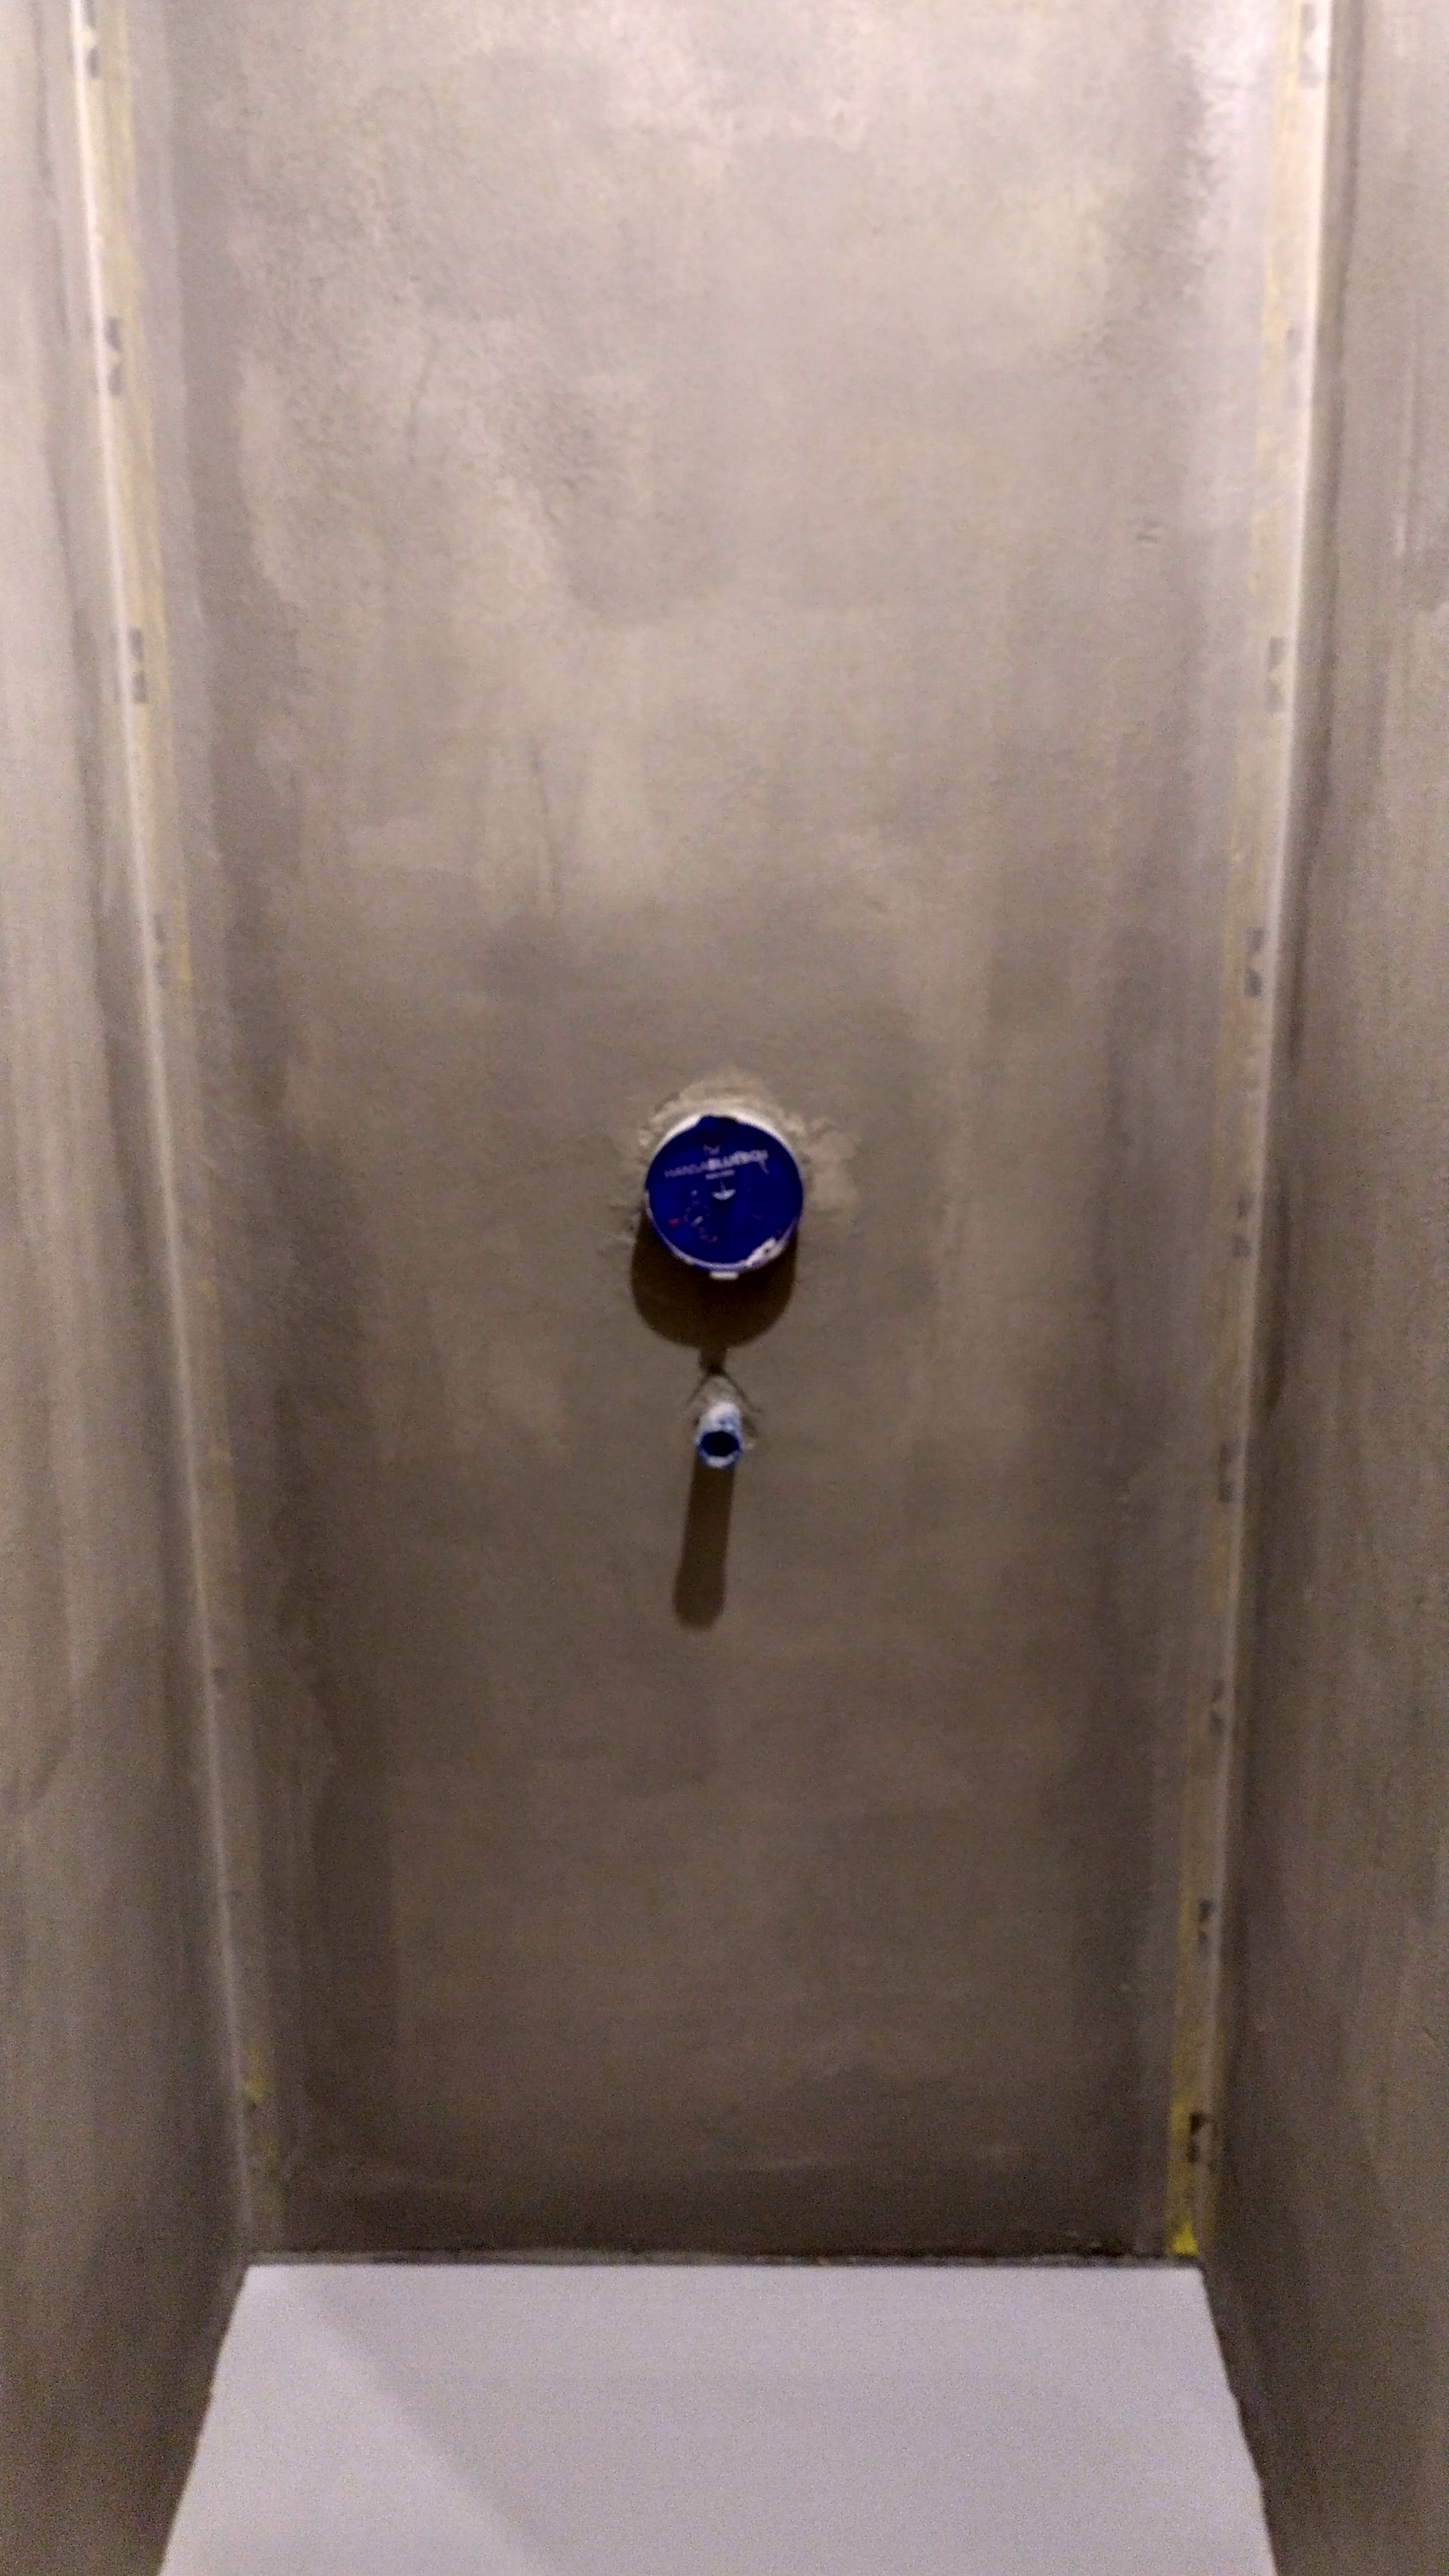
\includegraphics[scale=0.1]{Resources/Praktikum/IMG_20180801_114911_HDR.jpg}
		\label{duscheDicht}
		\caption{Abgedichtete Dusche}	
	\end{center}
\end{figure}

\begin{figure}[h]
	\begin{center}
		\noindent\includegraphics[scale=0.1]{Resources/Praktikum/IMG_20180801_114820_HDR.jpg}
		\label{bodenDicht}
		\caption{Boden mit Entkopplungsmatten und Abdichtbändern in den Ecken}	
	\end{center}
\end{figure}

\begin{figure}[h]
	\begin{center}
		\noindent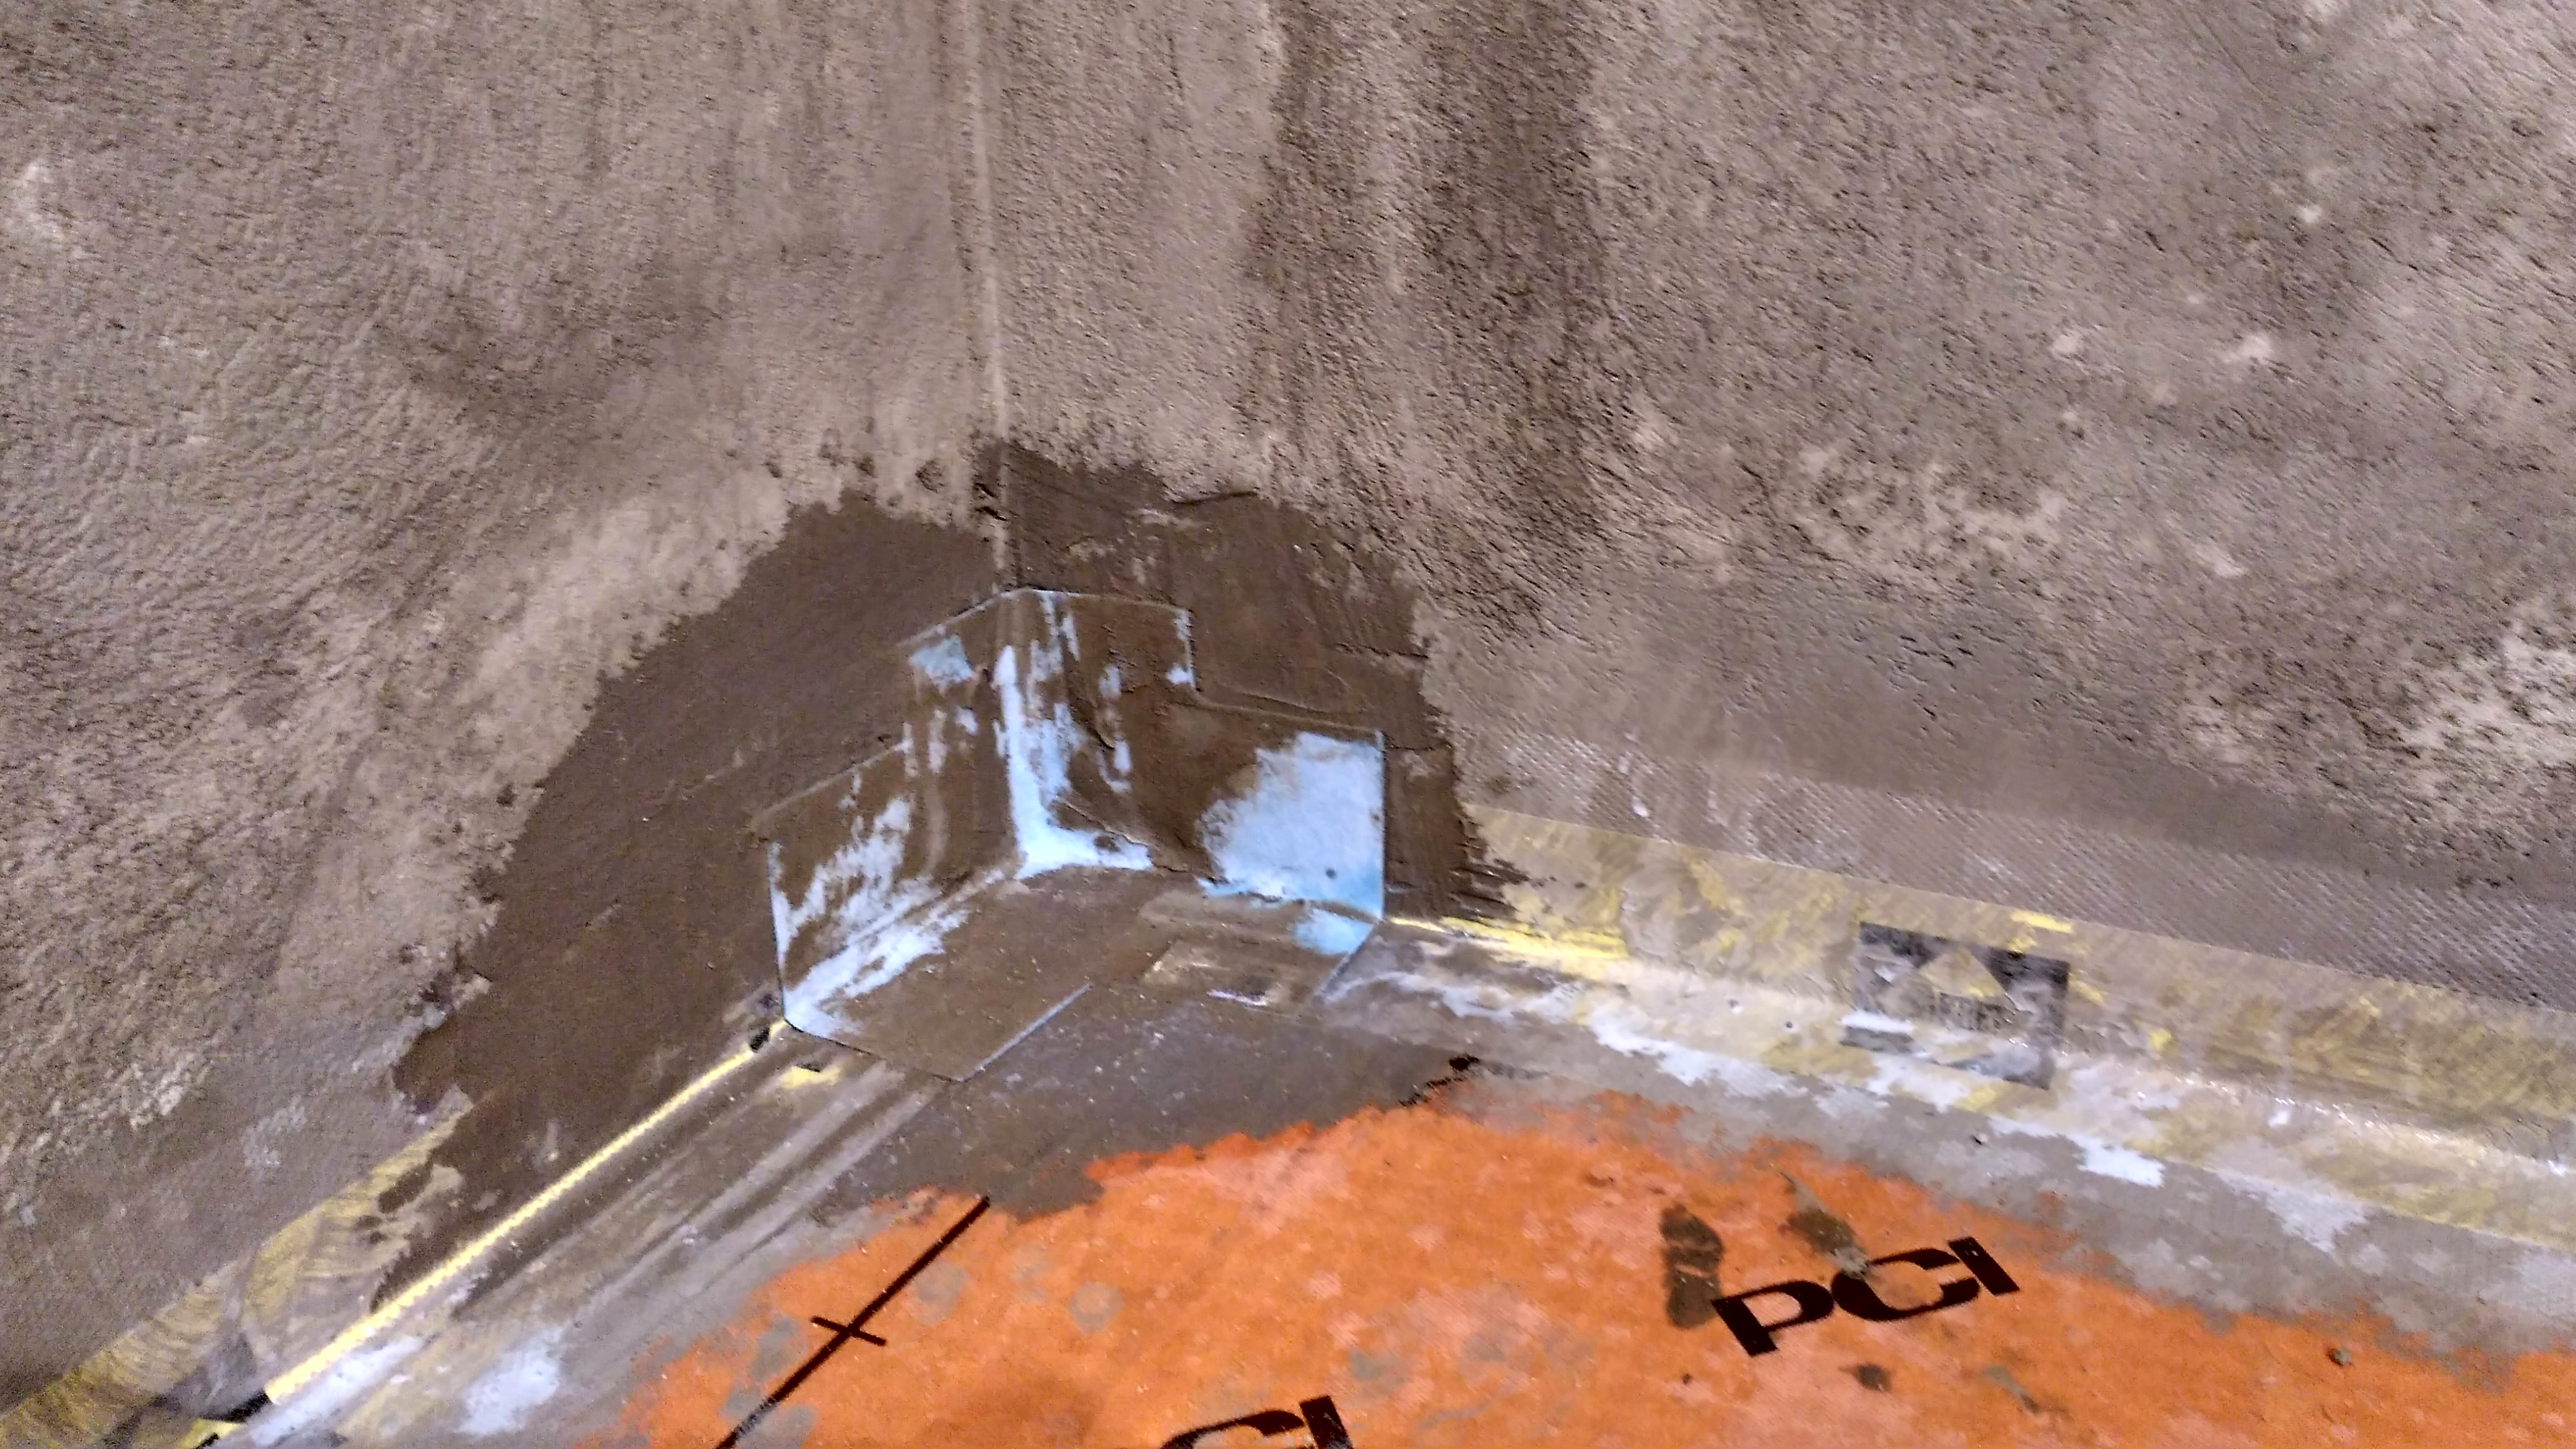
\includegraphics[scale=0.1]{Resources/Praktikum/IMG_20180801_114836_HDR.jpg}
		\label{eckeDicht}
		\caption{Ecke mit Abdichtbändern}	
	\end{center}
\end{figure}

Nun mussten die Wände der Dusche den Vorschriften gemäß wasserdicht gemacht werden. Nur Fliesen alleine bieten einen ungenügenden Schutz gegen Wasser. Dazu strich ich die gesamte Dusche mit Lastogum, einer Flüssigfolie aus. Diese bildet auf der Mauer eine Wasserundurchlässige Schicht. In den Kanten der Dusche mussten Abdichtbänder eingeklebt werden. Dazu schnitt ich nach Augenmaß die Bänder zurecht. Anschließend strich ich dick Flüssigfolie in die Kanten und klebte das Abdichtband ein (siehe Abbildung \ref{duscheDicht}). Währenddessen bestrich der Fliesenleger den Periplanboden mit Hilfe einer feinzahnigen Kelle mit Kleber und legte die Entkopplungsmatten darauf (siehe Abbildung \ref{bodenDicht}). Die Kelle mit 2mm Stärke benutzte er, damit er den Kleber nicht zu dick aufträgt, damit die Matte nicht schwimmt und wellig wird. Daraufhin klebte ich die Abdichtbänder auch in die Kanten des Bodens, auf die Entkopplungsmatten. Der Fliesenleger klebte danach noch Abdichtecken in alle Ecken des Raums, um ihn komplett wasserdicht zu machen (siehe Abbildung \ref{eckeDicht}). Anschließend grundierten wir den Boden und alle Wände. Dann war alles bereit zum Fliesenverlegen.

\subsection{Fliesen verlegen und verfugen}

Der Fliesenleger wollte zuerst die Wandfliesen verlegen. Dazu bestimmte er anfangs noch einmal ganz genau die Länge der ersten Wand. Er bestimmte zusätzlich ob der Boden entlang der Wand gerade verlief, oder ob sich Unebenheiten zeigten. Damit wollte der den Verschnitt bestimmen, den er am Boden haben wird, oder ob der, bei geradem Boden, ganze Fliesen bis nach unten verlegen konnte. Er wollte ca. auf Schulterhöhe mit dem Verlegen beginnen. Dazu zeichneten wir eine horizontale Orientierungslinie mit einer Schlagschnur an. Durch diese Linie konnte er sichergehen, dass die Wandfliesen nicht schief wurden, wenn er von einer Seite der Wand zur anderen verlegte. Er strich mit einer gezahnten Kelle Kleber, genug für zwei aneinanderliegende Fliesen, an die Wand und klebte eine Fliese ein. Beim Einkleben der zweiten Fliese ließ er für die Fuge ca. 5mm Platz zur ersten Fliese. Das machte er nach Augenmaß, ohne Abstandshalter. So klebte er eine Linie Fliesen vom einen Ende der Wand zum Anderen, entlang der Orientierungslinie ein. Bis jetzt konnte er dafür ganze Fliesen verwenden, die letzte musste er zuschneiden.

\begin{figure}[h]
	\begin{center}
		\noindent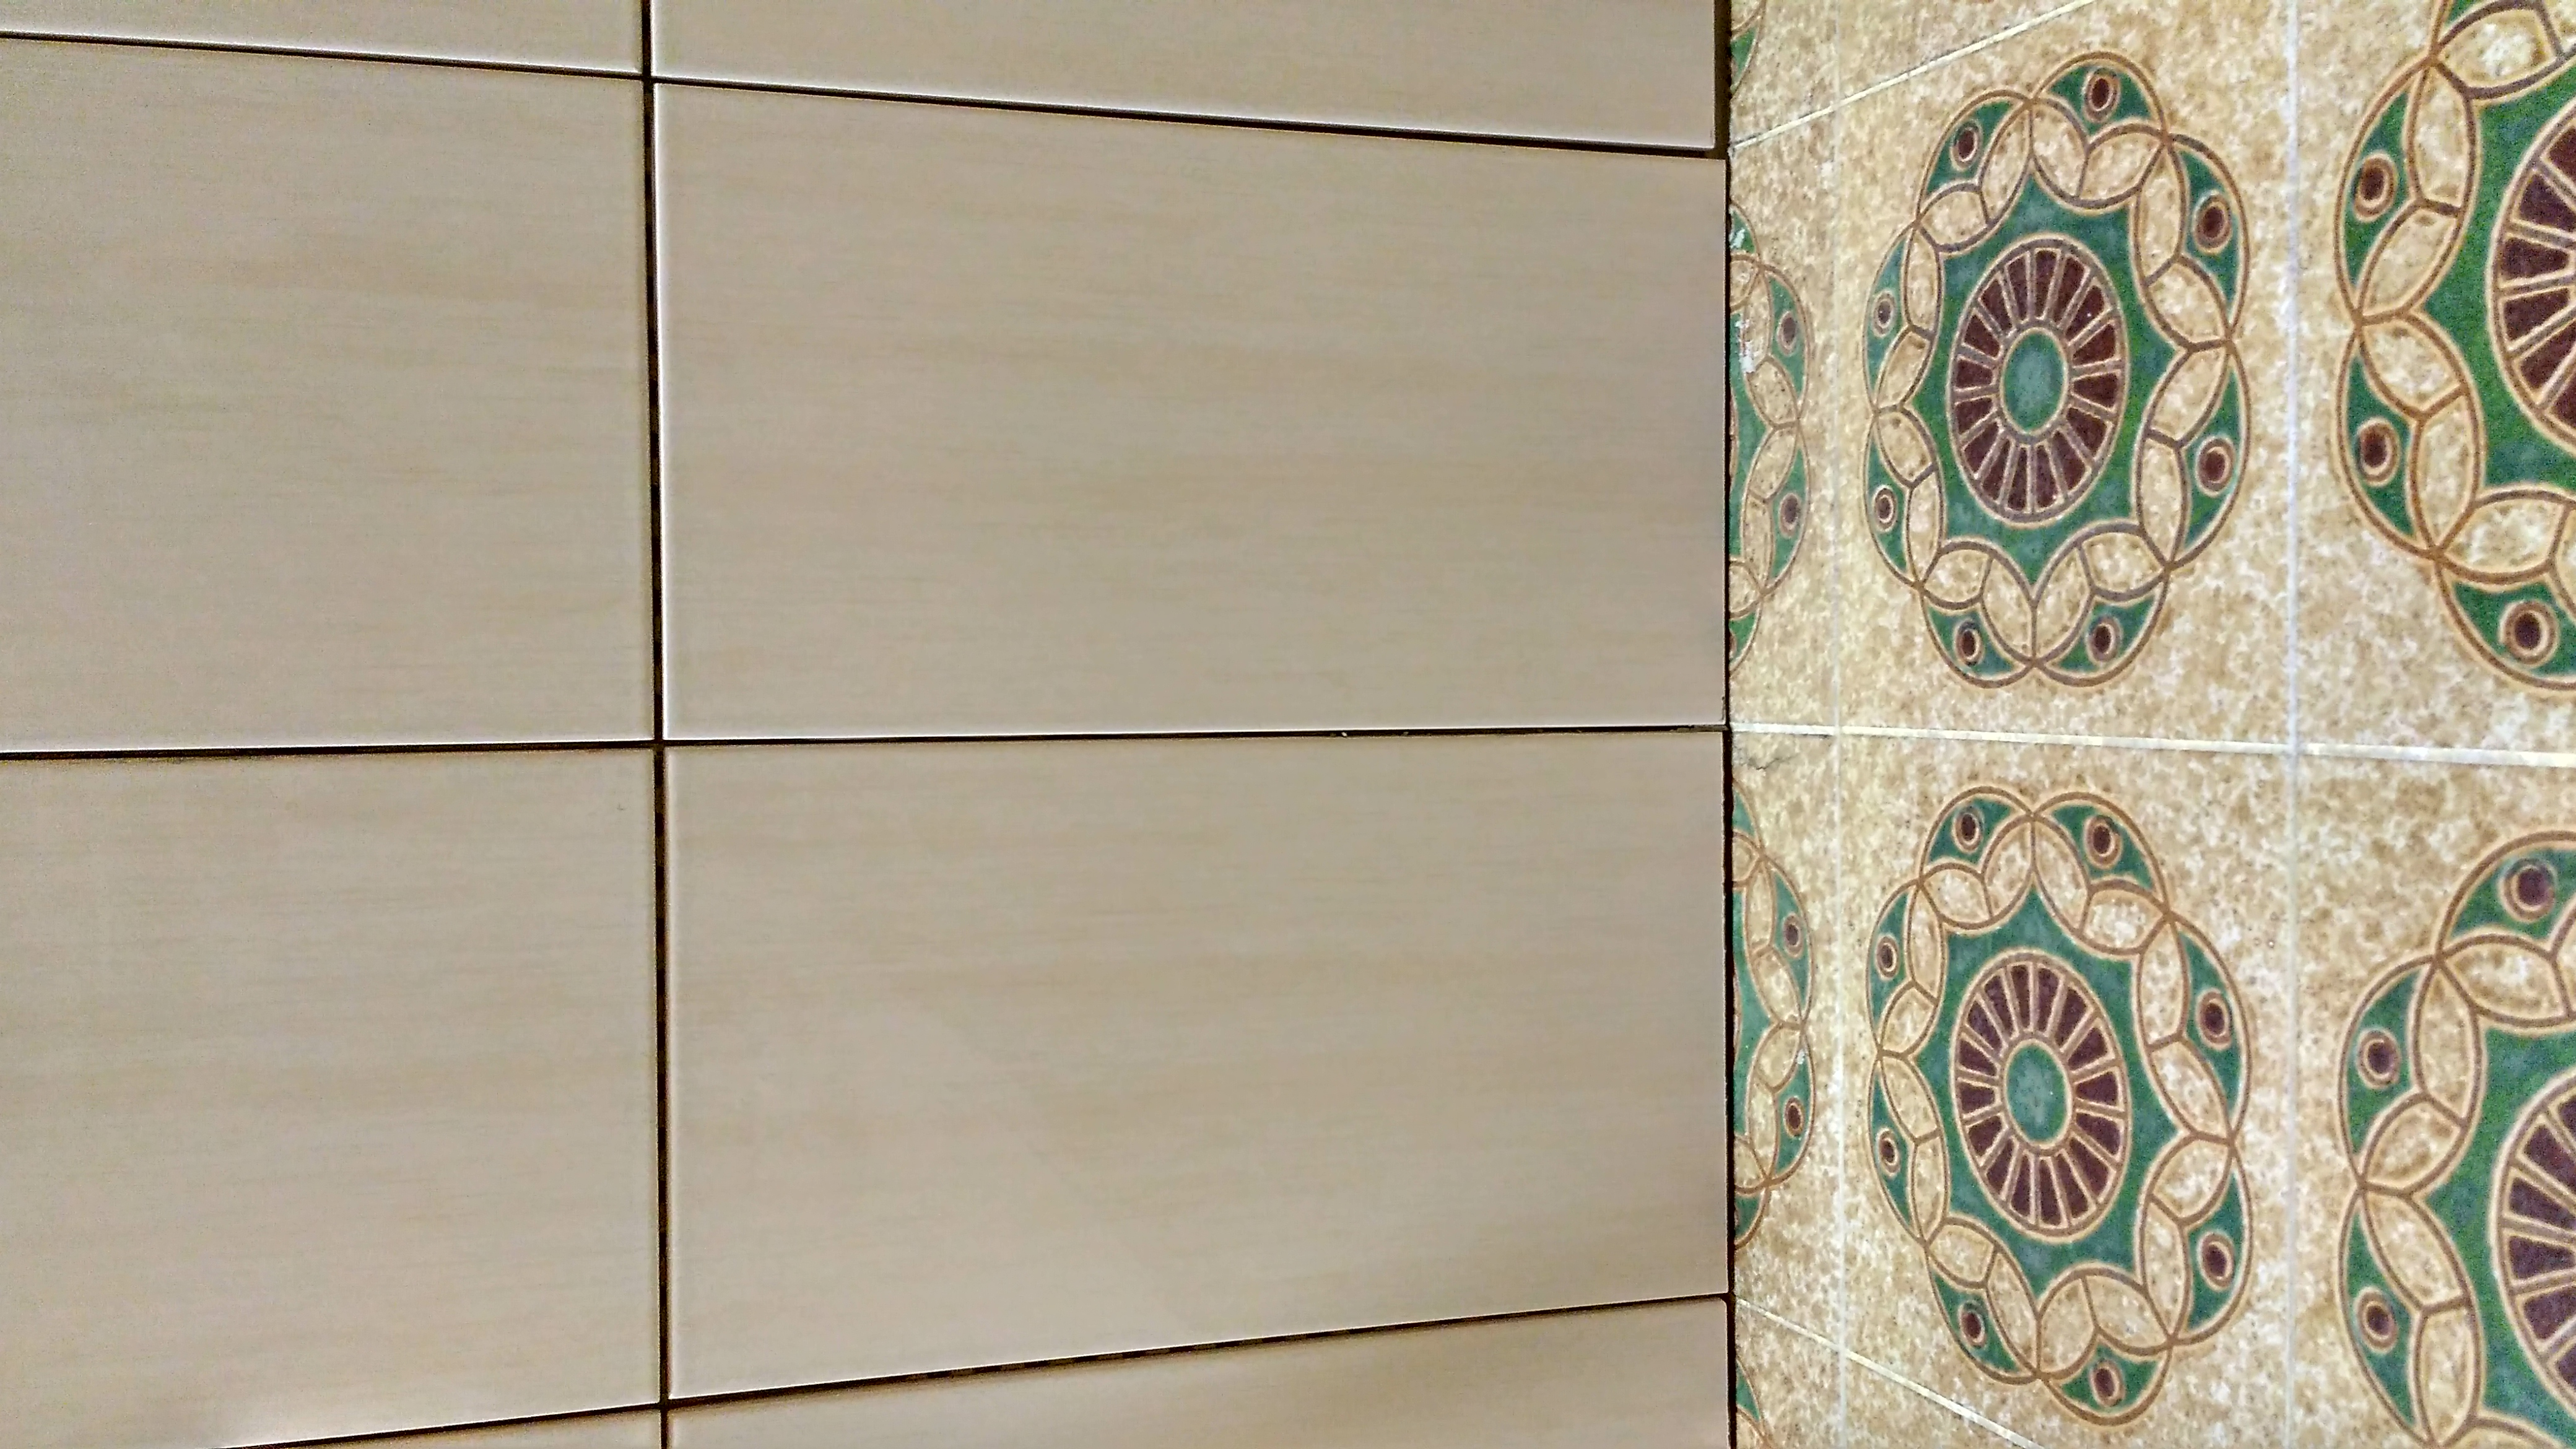
\includegraphics[scale=0.1]{Resources/Praktikum/IMG_20180806_081044_HDR.jpg}
		\label{wandFlieseSchneiden}
		\caption{Geschnittene Fliesen am Ende der ersten Wand}	
	\end{center}
\end{figure}

\begin{figure}[h]
	\begin{center}
		\noindent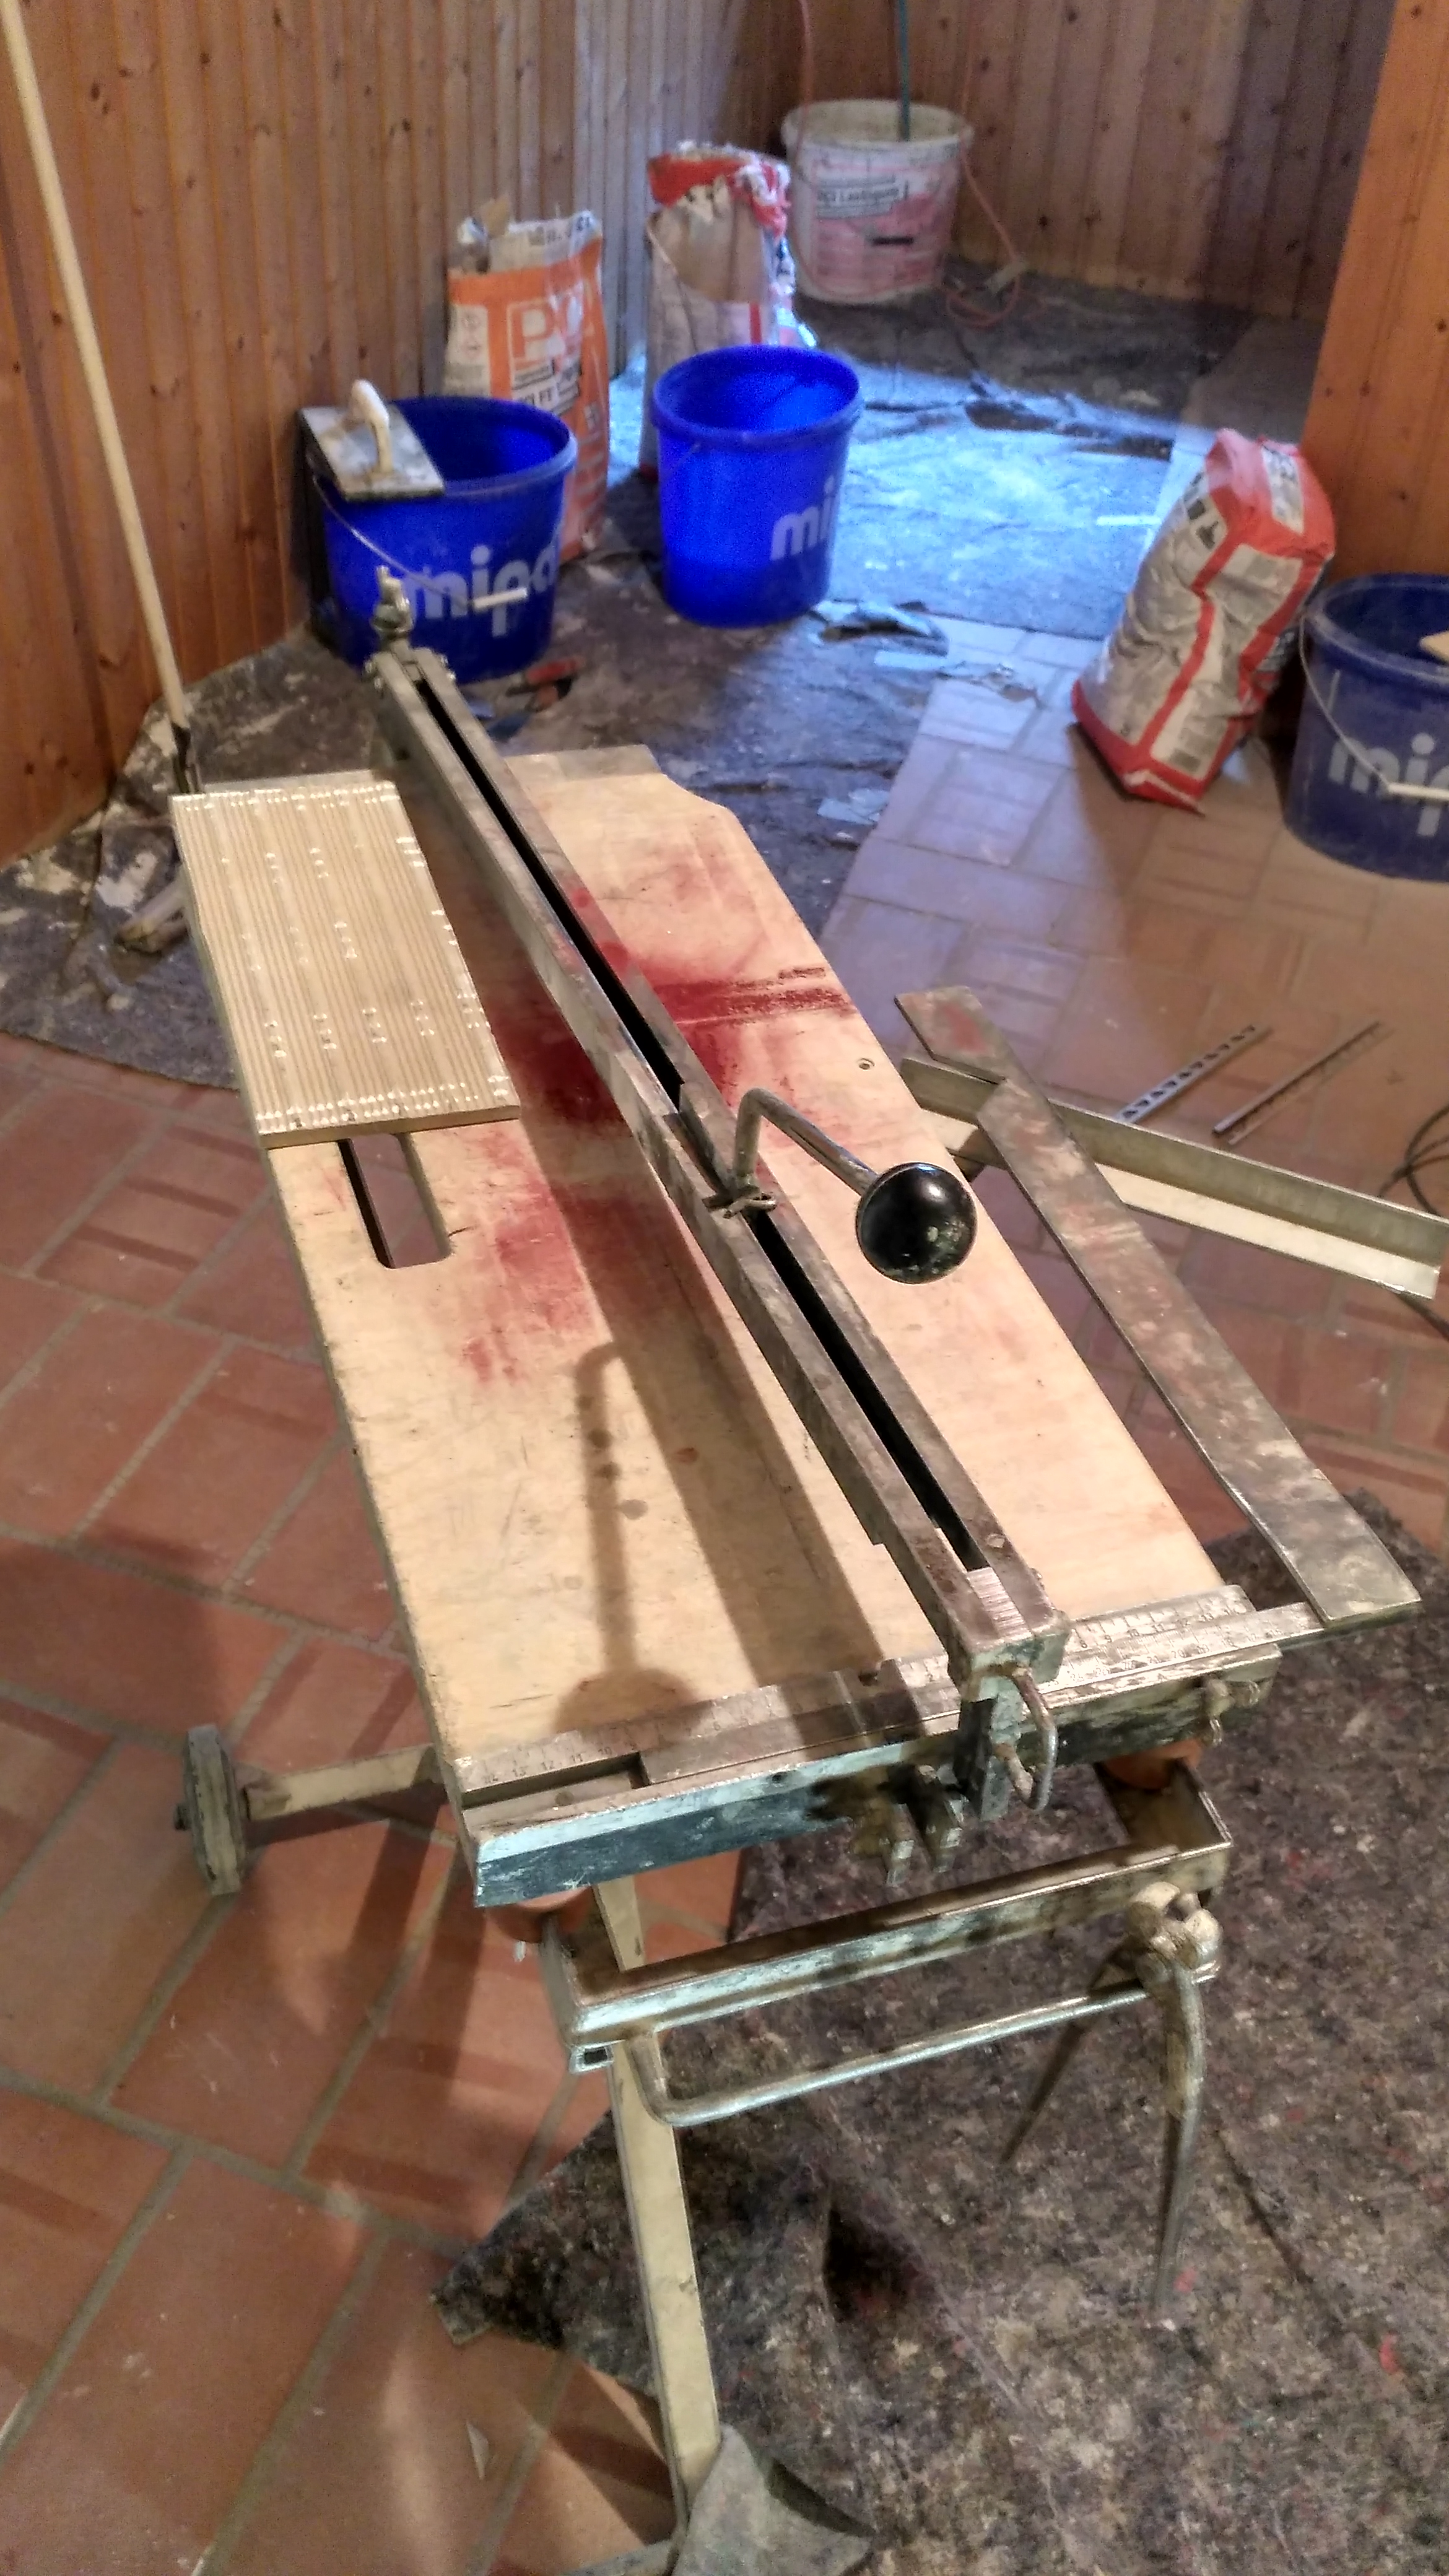
\includegraphics[scale=0.1]{Resources/Praktikum/IMG_20180807_120442_HDR.jpg}
		\label{schneider}
		\caption{Schneidebrett}	
	\end{center}
\end{figure}

Er maß den Abstand der letzten Fliese zur Wand. Auf seinem Fliesenschneider konnte er das Maß darauf einstellen, legte die Fliese ein, fuhr einmal mit dem Schneider darüber und brach das unbenötigte Stück entlang der Schnittlinie ab. Der gesamte Vorgang dauerte nicht länger als eine Minute.

Die zugeschnittene Fliese brachte er am Ende der Wand an. Anschließend klebte er die zwei Reihen darunter usw. ein (siehe Abbildung \ref{wandFlieseSchneiden}). Danach schlugen wir wieder eine horizontale Orientierungslinie an die Wand. Das machten wir regelmäßig, um zu gewährleisten, dass die Fliesenreihe nicht schief wurde. So flieste er die gesamte Wand, während ich ihm die Fliesen reichte.

\begin{figure}[h]
	\begin{center}
		\noindent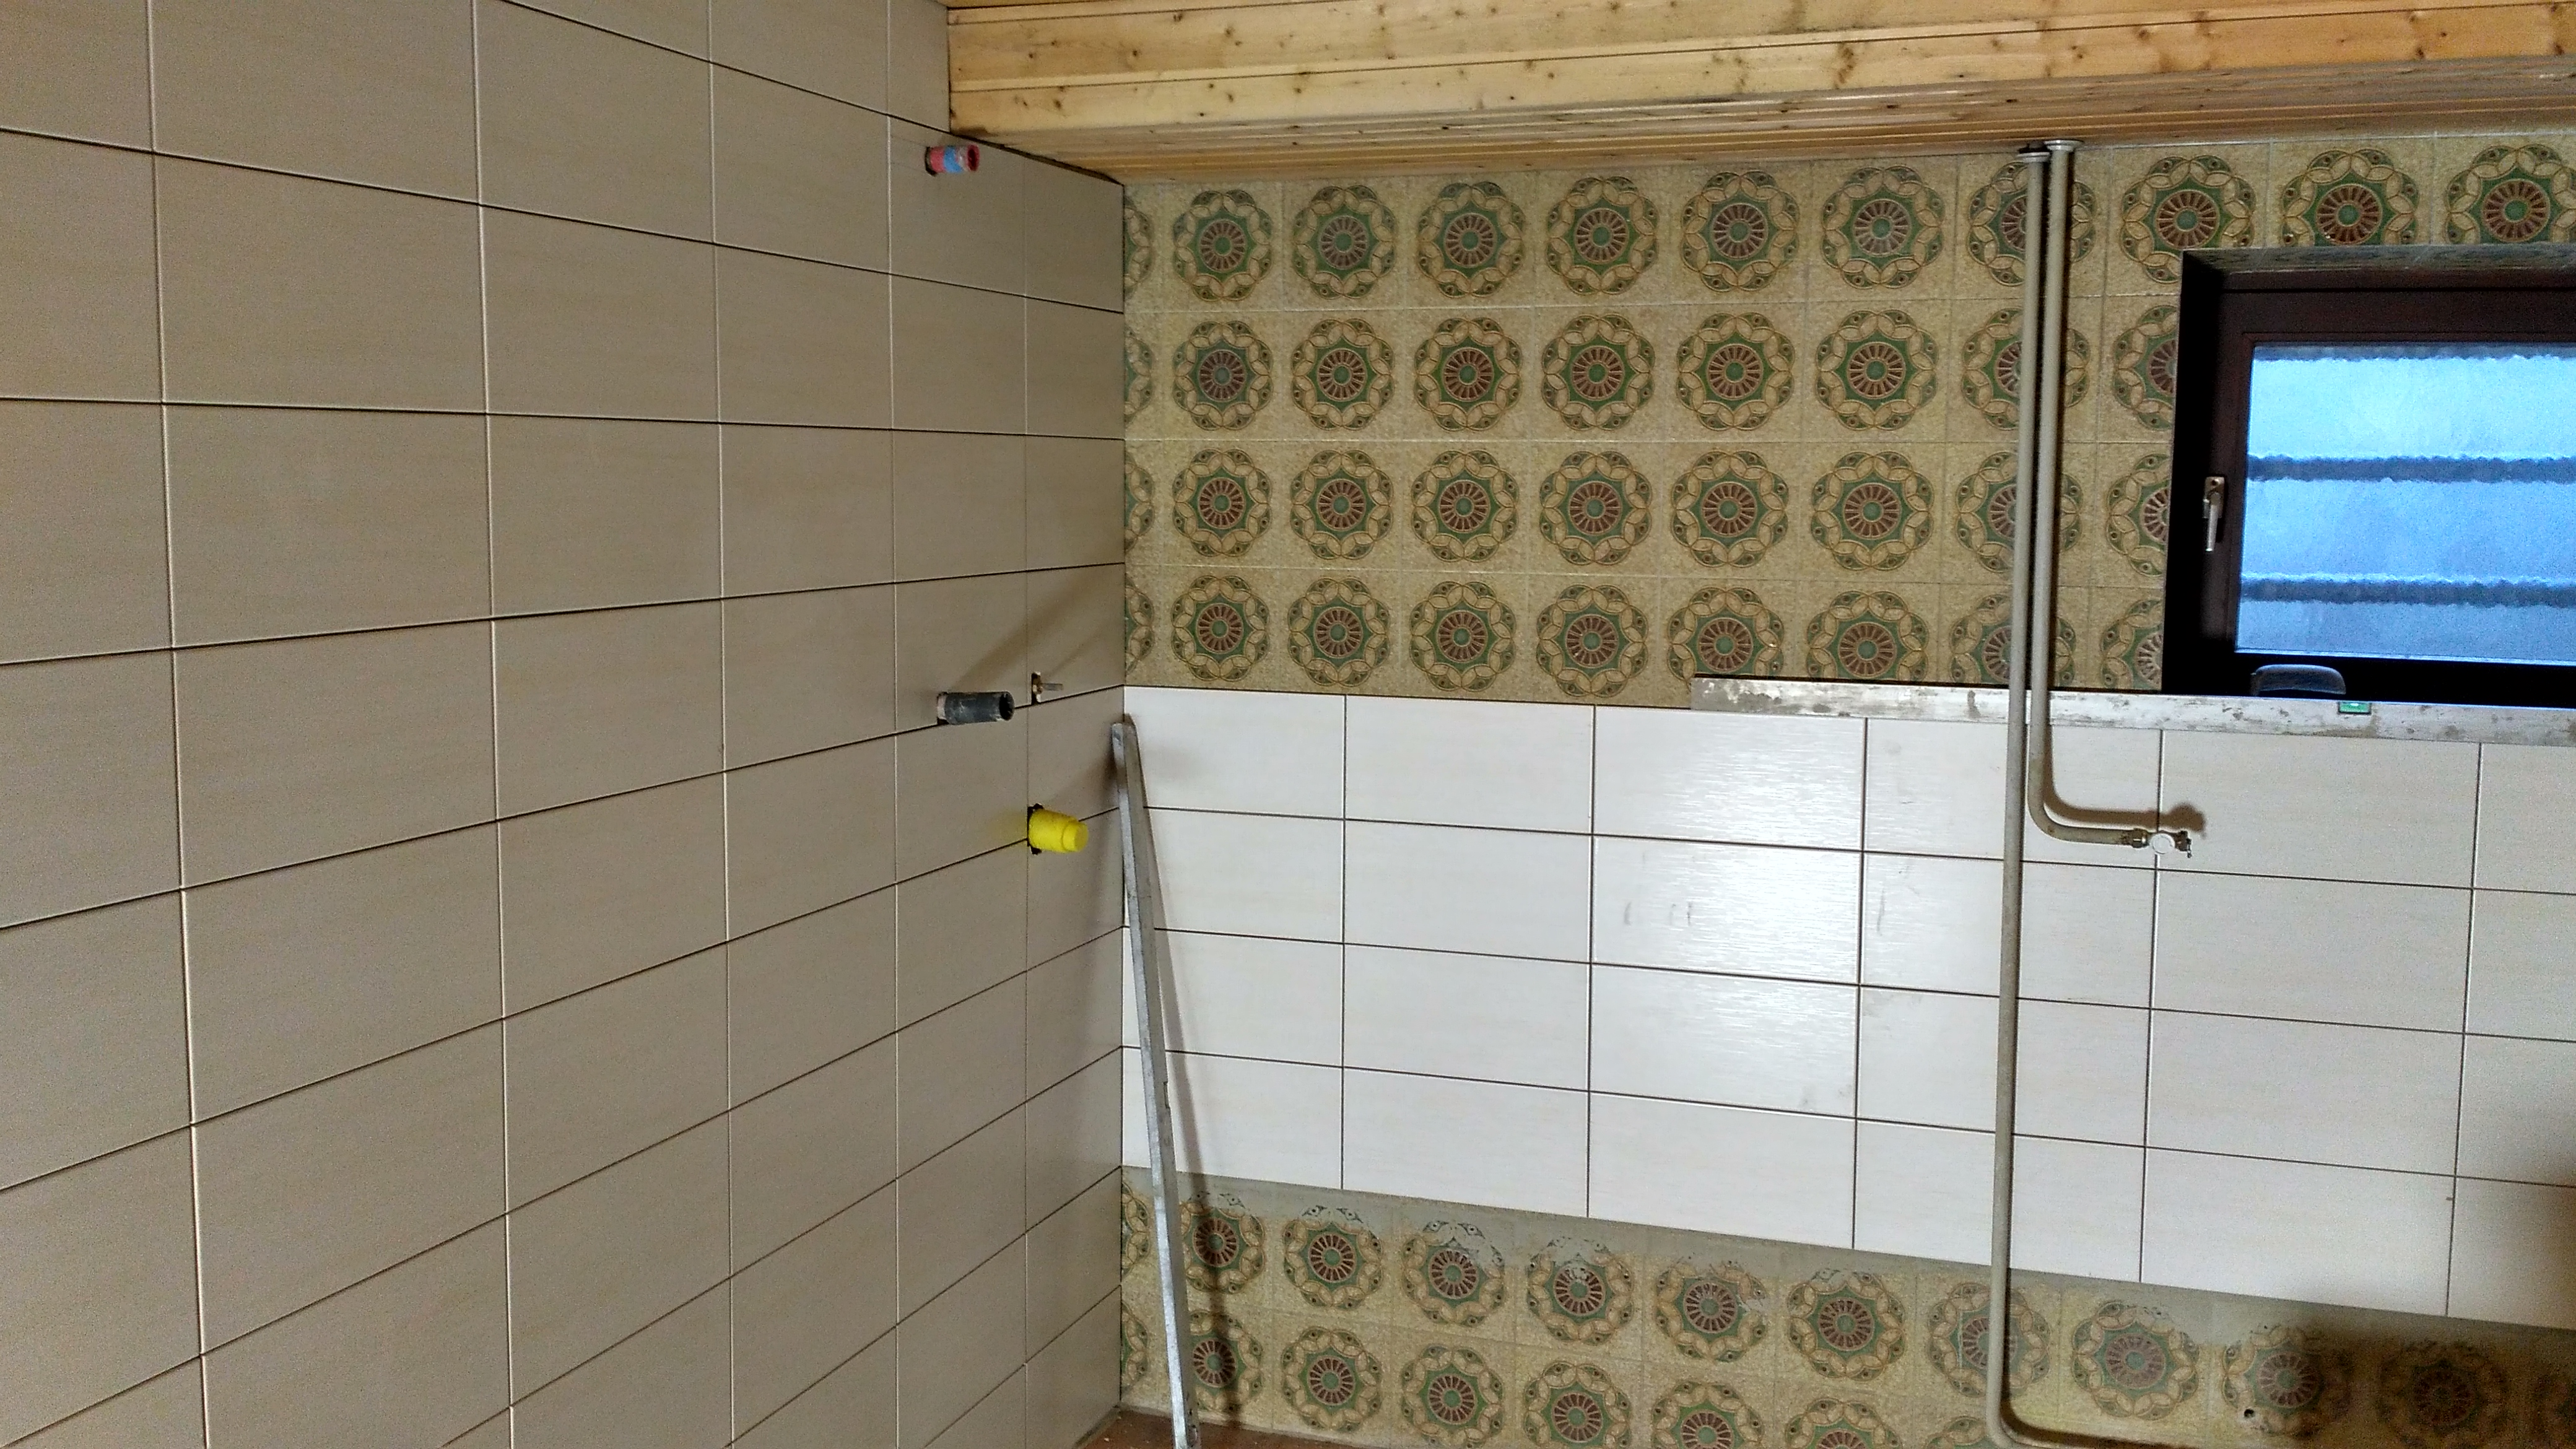
\includegraphics[scale=0.1]{Resources/Praktikum/IMG_20180806_081011_HDR.jpg}
		\label{ersteWand}
		\caption{Fertige erste Wand und Anfang der Zweiten}	
	\end{center}
\end{figure}

Sobald die erste Wand fertig verfliest war begann er mit den anderen und ich fing an die Fliesen zu verfugen. Dazu strich ich mit einer Kelle dick Fugenmasse in die Zwischenräume der Fliesen. Anschließend wischte ich mit einem feuchten Schwamm darüber, um die überschüssige Fugenmasse abzutragen und der Fuge ihr richtiges Aussehen zu geben. Zum Schuss zog ich den frisch ausgewaschenen Schwamm einmal komplett von oben nach unten über die Wand, um die Fliesen sauber zu waschen. So ging ich auch bei den anderen Wänden vor.

\begin{figure}[h]
	\begin{center}
		\noindent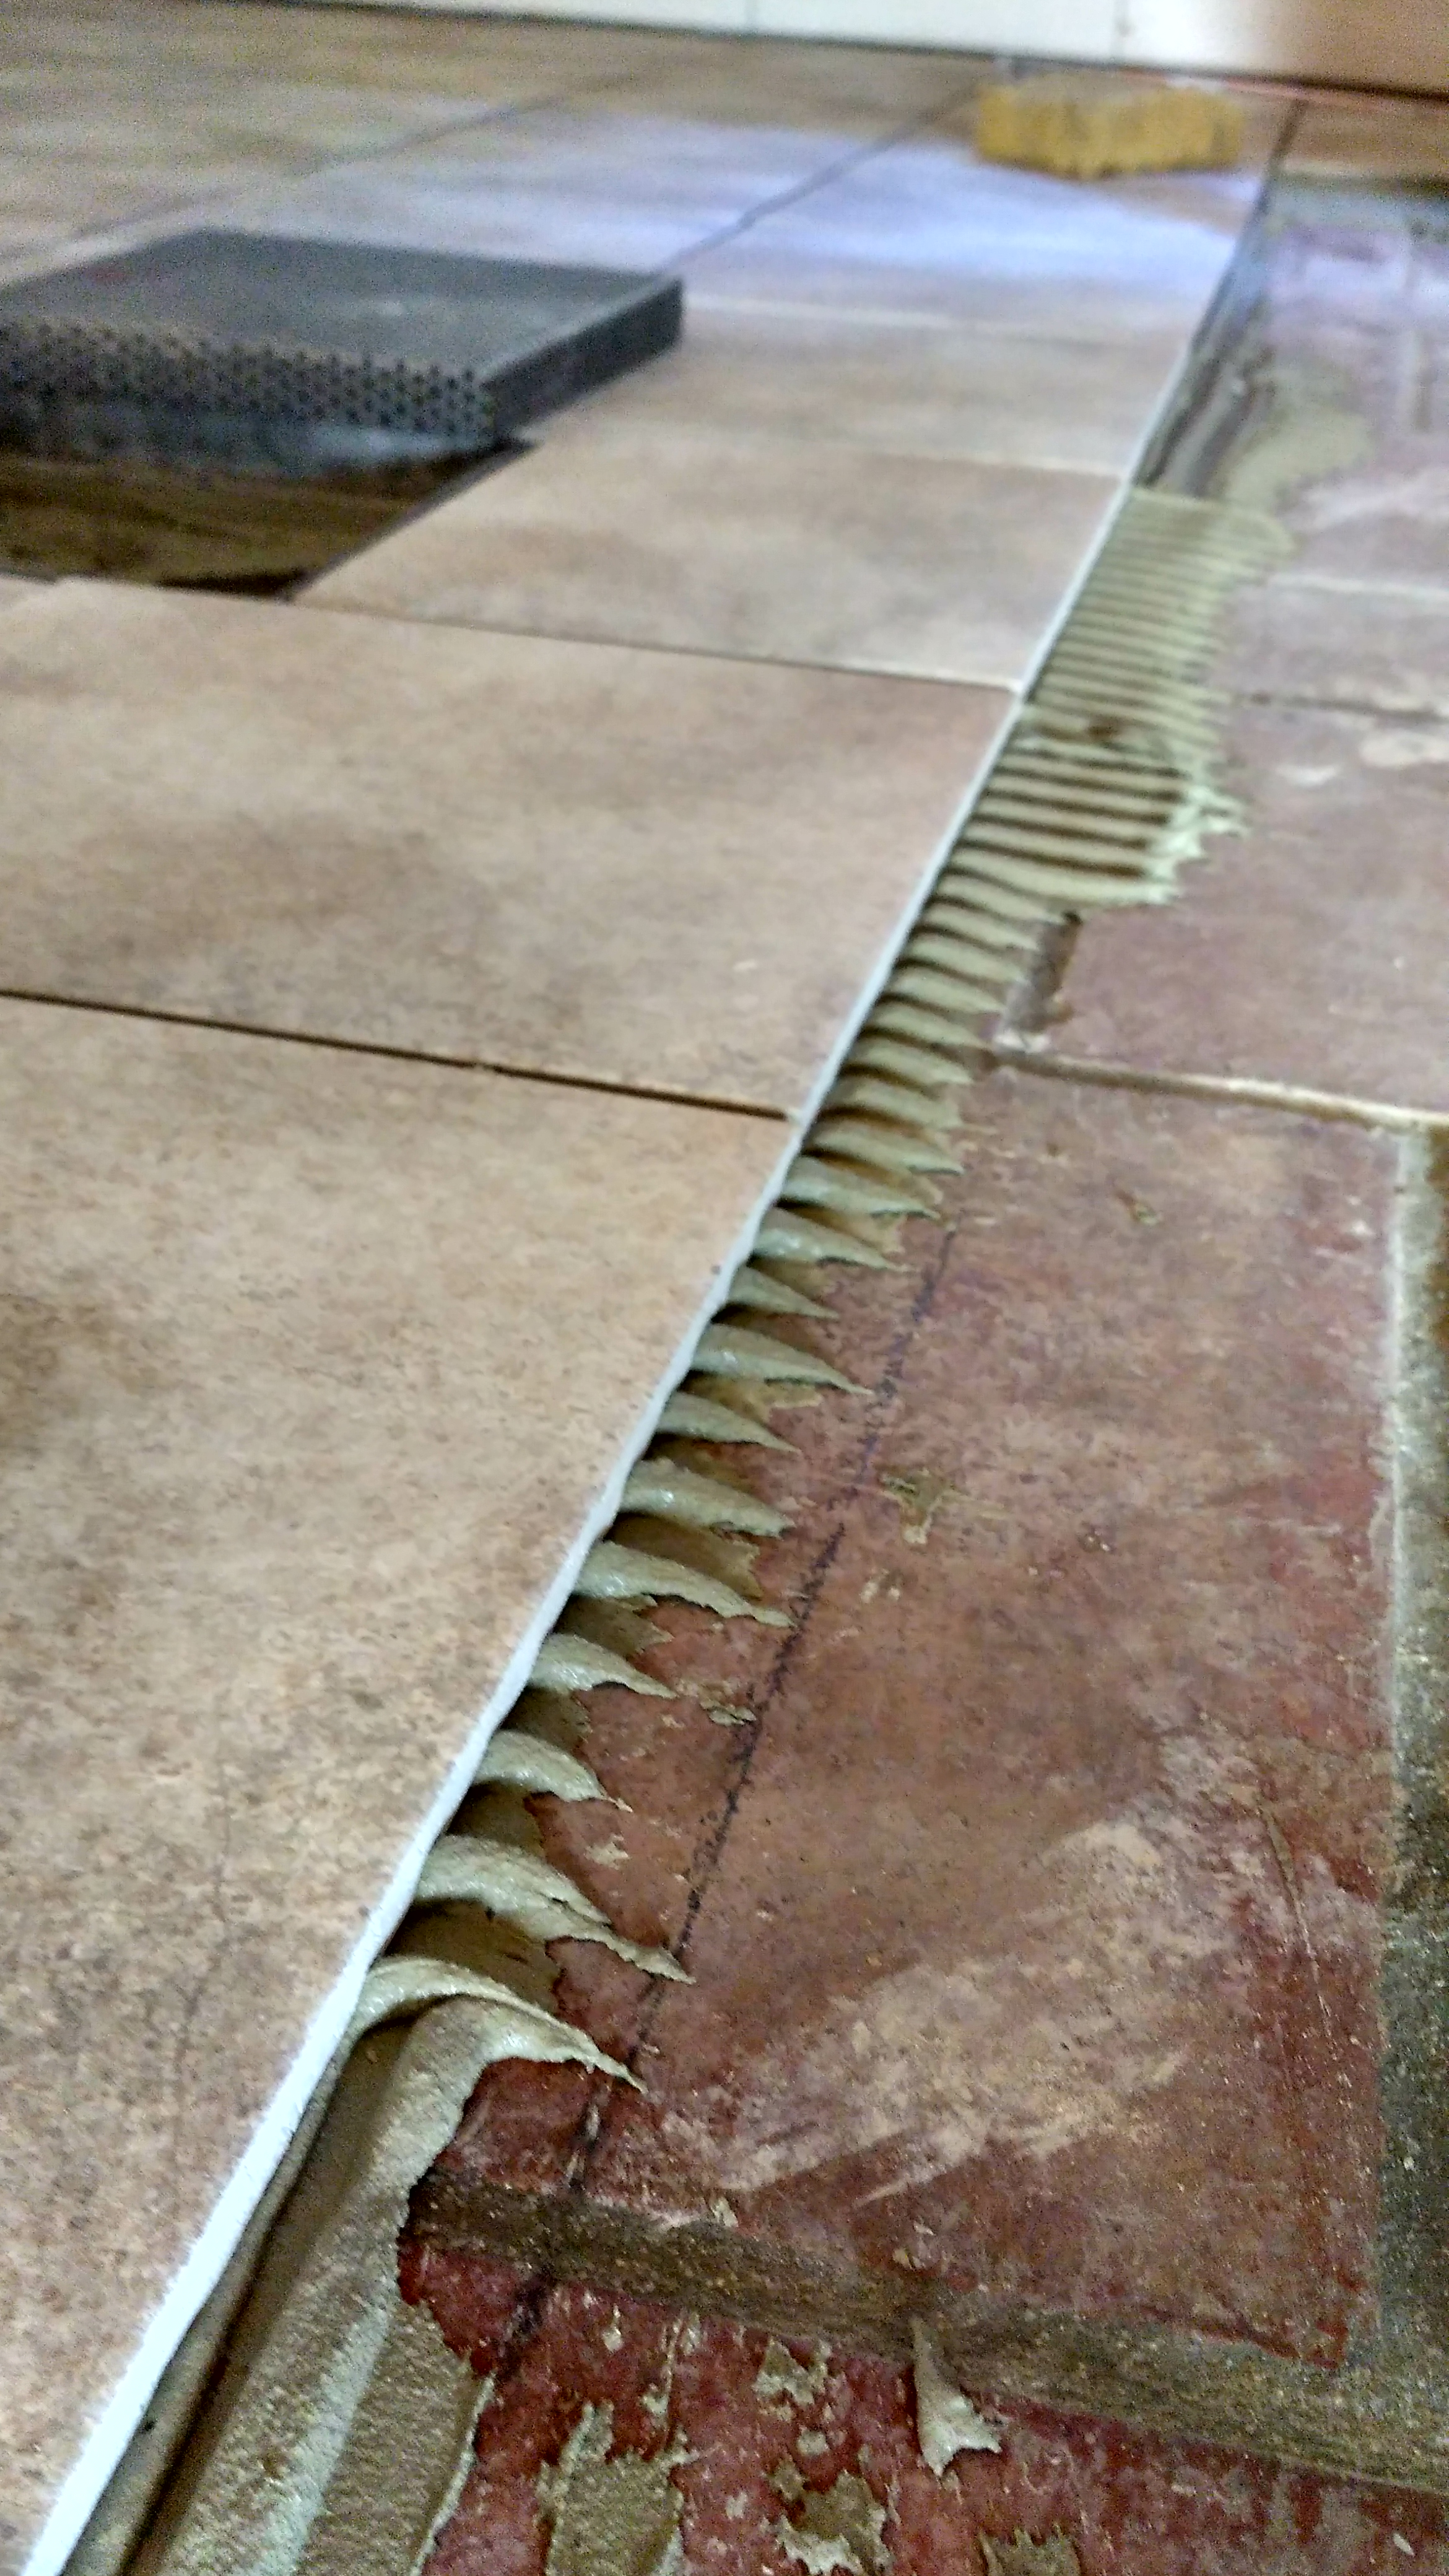
\includegraphics[scale=0.1]{Resources/Praktikum/IMG_20180807_112239_HDR.jpg}
		\label{orientierung}
		\caption{Orientierungslinie zum Verlegen der Bodenfliesen}	
	\end{center}
\end{figure}

Nach dem Verlegen der Wände begann er mit dem Boden. Durch den Periplanboden war sichergestellt, dass keine Unebenheiten vorhanden sind. Sollte die Mitte des Raumes beispielsweise einen Abfluss haben und man müsste den Boden zu diesem abfallen lassen, müsste der Fliesenleger das beim Verlegen mit einplanen. Hier hatten wir aber einen ebenen Boden. Nun zeichneten wir mit der Schlagschnur wieder eine Orientierungslinie parallel zur Wand ein, ca. so weit von dieser entfernt, wie die Breite zweier aneinandergelegter Fliesen (siehe Abbildung \ref{orientierung}). Ich platzierte einige Bodenfliesen so, dass der Fliesenleger direkt darauf zugreifen kann, während er am Boden kniet und die Fliesen verlegt. Er strich den Kleber auf den Boden und verteilte ihn mit einer gezahnten Kelle. Danach legte er die Fliesen darauf. Den Abstand zweier Fliesen für die Fuge bestimmte er per Augenmaß. Die Orientierungslinie diente dazu, dass die Fliesen nicht schief wurden, da er alles nach Augenmaß verlegte. 

Nachdem er zwei Reihen Fliesen verlegt hatte, stand er auf und wir zeichneten eine weitere Orientierungslinie, zwei Fliesenbreiten weiter, ein. Dann wiederholte sich der ganze Prozess, bis der Boden komplett verlegt war. Mir viel dabei auf, dass der Arbeitsfluss des Fliesenlegers durch das anzeichnen der Orientierungslinie immer wieder unterbrochen wurde. 

Zum Schluss, nachdem der Kleber eine Nacht ausgehärtet hatte, verfugte ich die Bodenfliesen noch. Dazu strich ich, wie beim Verfugen der Wandfliesen, Fugenmasse zwischen die Fliesen, wischte mit feuchten Schwamm darüber, bis sie das ge-wünschte Aussehen hatten und wusch die Fliesen anschließend mit dem Schwamm sauber. Nun war der gesamte Raum gefliest.

\subsection{Finale Schritte}

Nach dem Fliesen und Verfugen müssen noch ein paar kleine Schritte durchgeführt werden, um die Arbeit fertigzustellen. Wurden beispielsweise große, schwere Wand-fliesen verlegt, wurden Abstandshalter zwischen zwei Fliesen geklemmt, damit diese nicht zusammenrutschen und die Fuge so zerstören. Diese Abstandshalter müssen jetzt entfernt werden, und die Löcher in der Fuge geschlossen.

Die Fliesen wurden verlegt, bevor der Türstock eingebaut wurde. Nachdem dieser eingesetzt wurde, mussten die Zwischenräume zwischen Türstock und Fliesen verfugt werden. Dazu spritzte der Fliesenleger Acrylsilikon hinein und strich es mit einem Schaber glatt. Acrylsilikon hat die Eigenschaft, Farbe, mit welcher er überstrichen wird, aufzunehmen und so besser zu halten.

\subsection{Besorgungsfahrten}
Um den Lesefluss nicht zu unterbrechen, habe ich Besorgungsfahrten in den Baumarkt oder Fahrten in das Lager nicht aufgenommen. Hier möchte diese zwei Aspekte kurz beschreiben.

Der Fliesenleger hat ein privates Lager, in dem er nicht verbrauchte Materialien, seine Utensilien, wie Kellen und Eimer, und Werkzeuge, wie ein Multitool aufbewahrt. Den Lagerbestand hat er im Kopf. Am Anfang jedes Tages fuhren wir zuerst in das Lager und packten die nötigen Sachen ein. Da sein Auto nicht zu groß war, war die Tagesplanung wichtig, um unnötige Lagerfahrten während des Tages zu vermeiden.

Hatte er etwas nicht im Lager, was wir für die Baustelle brauchten, kauften wir es im Baumarkt ein. Alle Handwerker sind gut mit Baumärkten vernetzt. Sie können anrufen und vorbestellen. Die Baumärkte bereiten die Materialien dann vor, sodass man sie schnell abholen kann. Noch dazu speichern die Märkte die Daten des Handwerkers und können so direkt Abrechnungen erstellen und ihm zukommen lassen. Das spart wiederum Zeit, da man nicht zum Bezahlen in der Schlange stehen muss.

\section{Herausgearbeitete Ansatzpunkte}

Durch die Ethnographie zeigt sich, dass die meisten Arbeitsschritte eines Fliesenlegers relativ schnell auch präzise ausgeführt werden können. Kleber und sonstige Stoffe anzumischen erfordert keine Hilfe. Wände mit Flüssigkleber, Boden oder Wände mit Fliesenkleber und Fugen mit Fugenmasse zu bestreichen, lässt sich mit geeignetem Werkzeug präzise und schnell ausführen. Auch für das Schneiden und Einkleben der Fliesen sind die Maße schnell genommen und eingezeichnet. Der Fliesenleger hat eine einstudierte Routine und arbeitet dadurch zügig.
Allerdings werden zwei Ansatzpunkte deutlich, bei denen der Handwerker Unterstützung benötigt. Das sind die Planung mit dem Kunden im Kundengespräch, wobei Kunde und Fliesenleger gerne aneinander Vorbeireden, oder der Kunde sich das Ergebnis nicht vorstellen kann, sowie das Fliesenlegen, wo der Fliesenleger durch das anschlagen der Orientierungslinie aus dem Arbeitsfluss gerissen wird.

\subsection{Unterstützung beim Fliesenlegen}

Wenn der Fliesenleger ohne Orientierungslinie arbeitet, läuft er Gefahr, den Boden irgendwann schief zu verlegen. Ohne sie kann er also nicht arbeiten. Jedes mal wenn er diese mit der Schlagschnur anzeichnet, muss er aufstehen, die Endpunkte der Linie markieren und diese einzeichnen. Das wird nochmal schwerer, wenn er allein arbeitet, da man eine Schlagschnur mit zwei Personen leichter benutzen kann. Das anzeichnen reißt ihn zusätzlich aus seinem Arbeitsfluss. Könnte der Fliesenleger den Schritt des Anzeichnens einer Orientierungslinie umgehen, könnte er ungehindert weiterarbeiten, sofern er einen Helfer hat der ihm die Fliesen reicht und Kleber für ihn anrührt. Dadurch kann er viel Zeit sparen und es wäre gleichzeitig auch bequemer für ihn.

\subsection{Unterstützung beim Kundengespräch}

Das Kundengespräch war chaotisch und sehr unstrukturiert. Die Vorstellungskraft der Kunden, vor allem wenn diese Laien sind, ist sehr begrenzt. Dadurch ist es schwer mit ihnen über Änderungen zu diskutieren. Der Fliesenleger hat das Bild, durch seine Erfahrung besser im Kopf. Jedoch ist es schwer das in Worte zu fassen die der Kunde versteht. Es wäre deutlich einfacher über Ideen zu sprechen, wenn man diese direkt vor sich sehen würde.

Das Ergebnis vorab schon zu sehen hat noch weiter Vorteile:

\begin{itemize}
	\item Der Kunde kann während dem Planungsprozess bereits gezielt Feedback geben. Ansonsten kann er das erst spät im Prozess, wodurch es erheblich schwerer ist darauf einzugehen.
	\item Dadurch kann der Vertrag mit dem Kunden, was der Fliesenleger zu tun hat, genauer ausgearbeitet werden.
	\item Die Zusammenarbeit mit anderen Handwerkern ist einfacher koordinierbar.
	\item Das geplante Muster dient als visuelle Vorlage für den Fliesenleger. Dadurch muss er das Bild nicht nur im Kopf haben.
	\item Bereits beim Planen des Raumes lässt sich der Verschnitt gut abschätzen.
\end{itemize}

Die Unterstützung bei der Orientierungslinie würde dem Fliesenleger Zeit ersparen und ein Visualisierungstool würde ihm die Planung erleichtern. Daran kann man ansetzen, um technische Unterstützungssysteme zu implementieren.
\chapter{Research}
\section{Beispiele für Technologisch gestützte Dienstleistungen}
\subsection{Heidelberger Druckmaschinen}
Heidelberger Druckmaschinen, allgemein bekannt als Heidelberg, ein Hersteller hochwertiger Druckmaschinen hat über den Lauf seiner Geschichte eine Vielzahl an Reparaturservices bereitgestellt.
Vor einigen Jahren, als Ihnen die Möglichkeiten des \enquote{Remote-Monitoring} eröffnet wurden, fanden Sie viel kosteneffizientere Methoden zur Reparatur der Maschinen.
Heute kommunizieren die Druckmaschinen direkt über das Internet und verbinden somit Heidelberg's Technischer-Support-Spezialisten mit den Druckmaschinen der Kunden.
Somit können die Druckprozesse der Klienten von Heidelberg aus der Ferne eingesehen und optimiert werden.
Der Produktsupport umfasst außerdem noch das Entfernen sowie das Weiterverkaufen von Druckmaschinen.
\\
Dieses Ausmaß von Vernetzung hat es Heidelberg möglich gemacht eine intime Verbindung mit ihren Kunden herzustellen.
Die Entlohnung dafür ein Smart Service Anbieter zu werden ist nicht zu Verneinen, denn mit einer solchen Kunden-Intimität wird auch großes Vertrauen in den Kunden aufgebaut.
\subsection{}





% Optimierung für Literaturverzeichnis
\setcounter{biburllcpenalty}{8000}
\setcounter{biburlucpenalty}{8000}

% Literaturverzeichnis generieren.
% Inhalt erscheint, sobald Einträge in der Bib hinterlegt sind!
\cleardoublepage
\addcontentsline{toc}{chapter}{Literaturverzeichnis}
\printbibliography[title={Literaturverzeichnis}]

% Abbildungsverzeichnis generieren.
\cleardoublepage
\addcontentsline{toc}{chapter}{\listfigurename}
\listoffigures


% Tabellenverzeichnis generieren.
%\cleardoublepage
%\addcontentsline{toc}{chapter}{\listtablename}
%\listoftables

% Listingverzeichnis generieren.
\cleardoublepage
\renewcommand{\lstlistlistingname}{Listingverzeichnis}
\addcontentsline{toc}{chapter}{\lstlistlistingname}
\lstlistoflistings

%
%% Anhang einfügen.
%\cleardoublepage
%\begin{appendix}
\chapter{<Kapitel im Anhang>}
Hier kommt der Anhang rein ...
\end{appendix}

% Glossar generieren
\glsaddall
\printglossaries

\end{document}
